\graphicspath{{content/chapters/5_evaluation/figures/}}

\chapter{Evaluation}%
\label{chp:evaluation}
\rule{\textwidth}{1pt} \\[1ex]

\epigraph{\textit{``It is not the strongest of the species that survive, nor the most intelligent, but the one most responsive to change.''}}{\textbf{-- Charles Darwin}}

\section{Introduction}
\label{sec:5_introduction}
% Grazzi Sinjur Alla, Ahfirli Sinjur Alla, u Ismaghni Sinjur Alla. Grazzi Amen

\section{Hardware Setup}
\label{sec:5_hardware_setup}

All experiments involving deep learning models were conducted using two primary hardware configurations. Training was performed on systems equipped with an NVIDIA GeForce RTX 4070 and an RTX 4090 \gls{gpu}, both supporting \gls{cuda}-enabled acceleration. These setups were used across different experiments as needed, enabling parallel computation and helping to reduce training times significantly. Furthermore, a batch size of 16 was consistently used across all experiments for training the deep learning models.


\section{Optimal Tiling Experiments}
\label{sec:5_tiling_exp}
% Glorja lil Missier, lil-Iben u lil- Ispirtu s-Santu, Kif kien fil bidu, issa u dejjem, ghal-dejjem. Amen. Grazzi Mulej
% all altitudes aggregated, since we require a detection model capable of generalising to different altitudes, definition of objects

%IMP Uncomment figures as you go along
To determine the most suitable tiling parameter for pre-processing the \gls{soda} dataset, which serves as an essential preliminary step in addressing objectives \textbf{O1}, \textbf{O2}, and \textbf{O3}, a series of experiments was conducted. The objective was to identify an appropriate grid size for effective tiling. Although the authors in \cite{detect_litter} proposed a 5$\times$5 configuration, they offered no clear justification for selecting that specific size.
Tiling is applied in this context to magnify the size of small litter objects, which appear relatively diminished due to the high-altitude perspective (see Figure \ref{fig:tiling_examples}). As the grid becomes finer, these objects occupy a larger proportion of each tile. This can potentially improve detection accuracy. A larger grid size, therefore, appears beneficial in this respect.

However, increasing the grid size introduces new challenges. The most significant issue is the additional burden on processing and inference time. More tiles are produced, which in turn means more data needs to be handled during model inference. This added complexity can lead to slower performance if not carefully managed \cite{tiling}.
Thus, choosing a grid size involves balancing two competing goals. One is to make small objects more detectable. The other objective is to prevent a significant rise in computational cost. Identifying an optimal balance between object visibility and processing efficiency requires further exploration.

In this study, an experiment was carried out to identify the optimal tiling grid size by measuring the rate of change in the number of small objects and the number of resulting images as the grid size increases. The first step involved establishing a classification scheme for object sizes. For this purpose, the definitions provided by the \gls{coco} dataset \cite{coco} were adopted, and are summarised below:

\begin{adjustwidth}{4em}{0pt} % Indent 2em from the left
\begin{description}
    \item[Small:] Objects occupying an area of less than $32 \times 32$ pixels.
    \item[Medium:] Objects with sizes ranging from $32 \times 32$ to $96 \times 96$ pixels.
    \item[Large:] Objects exceeding $96 \times 96$ pixels in area.
\end{description}
\end{adjustwidth}

With these definitions in place, the experiment proceeded by testing a range of grid sizes from 1 to 10. A grid size of 1 represents the original image with no tiling applied, while a grid size of 10 results in each image being divided into 100 tiles. For each configuration, the rate of change was recorded for small, medium, and large objects, as well as the total number of annotations and images.
A key consideration was the treatment of annotations that spanned tile boundaries. In such cases, these annotations were duplicated across the relevant tiles, leading to an expected increase in annotation count. This effect was deliberately preserved to reflect how tiling may influence the volume of training data. Each tile was also resized to 800 by 800 pixels to ensure consistency in size across all tiling configurations. This resizing was essential for maintaining uniform object scale during analysis, as 800 pixels was the chosen model input size throughout this study (refer to Subsection \ref{subsec:4_resizing}).

\begin{figure}[!ht]
  \centering
  \begin{tabular}{c}
    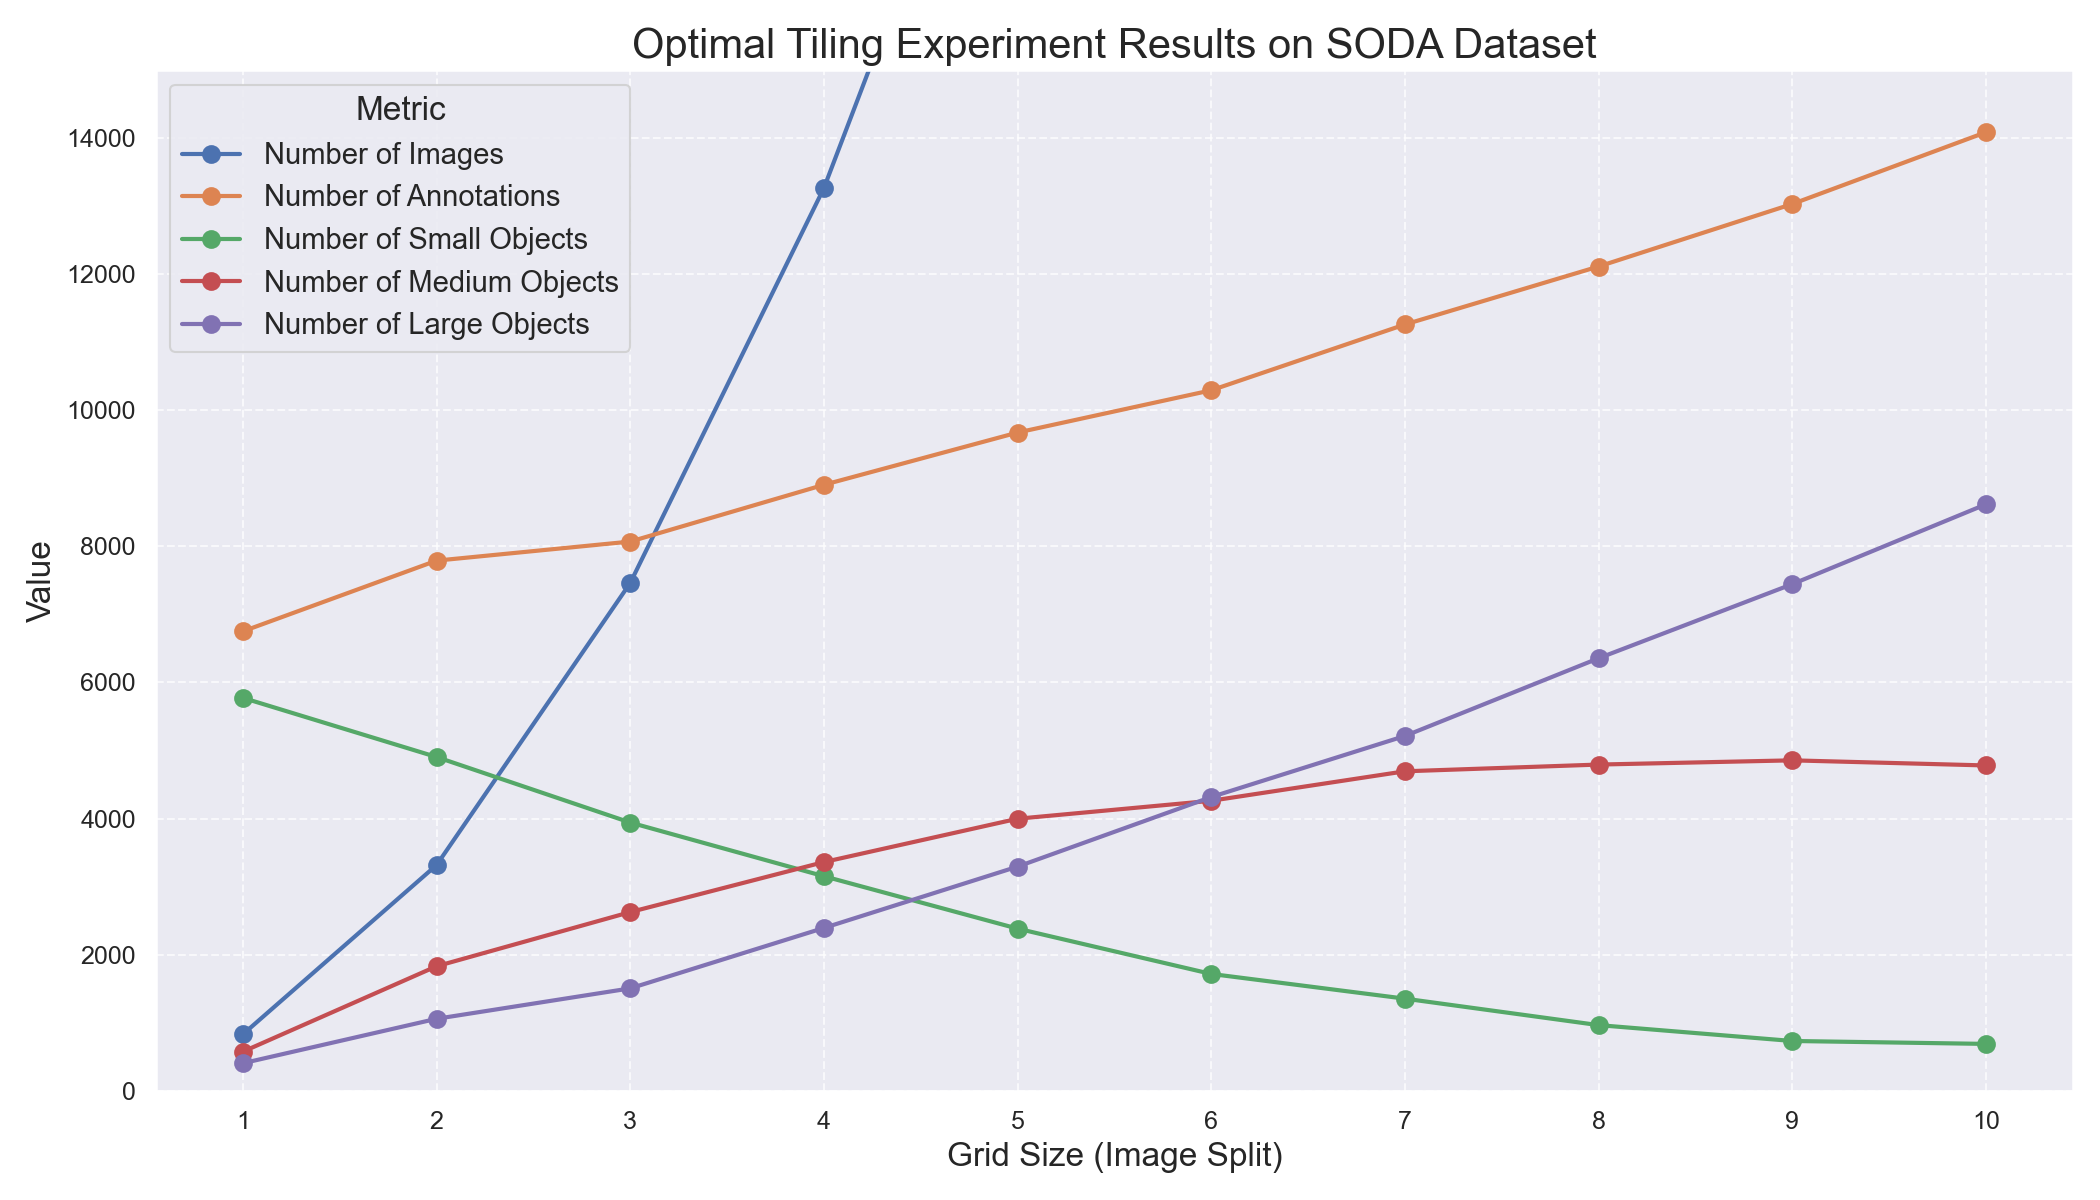
\includegraphics[width=0.9\textwidth]{optimal_tiling_experiment_results_line1.png} \\
    \small (a) \\
    \addlinespace[1em]
    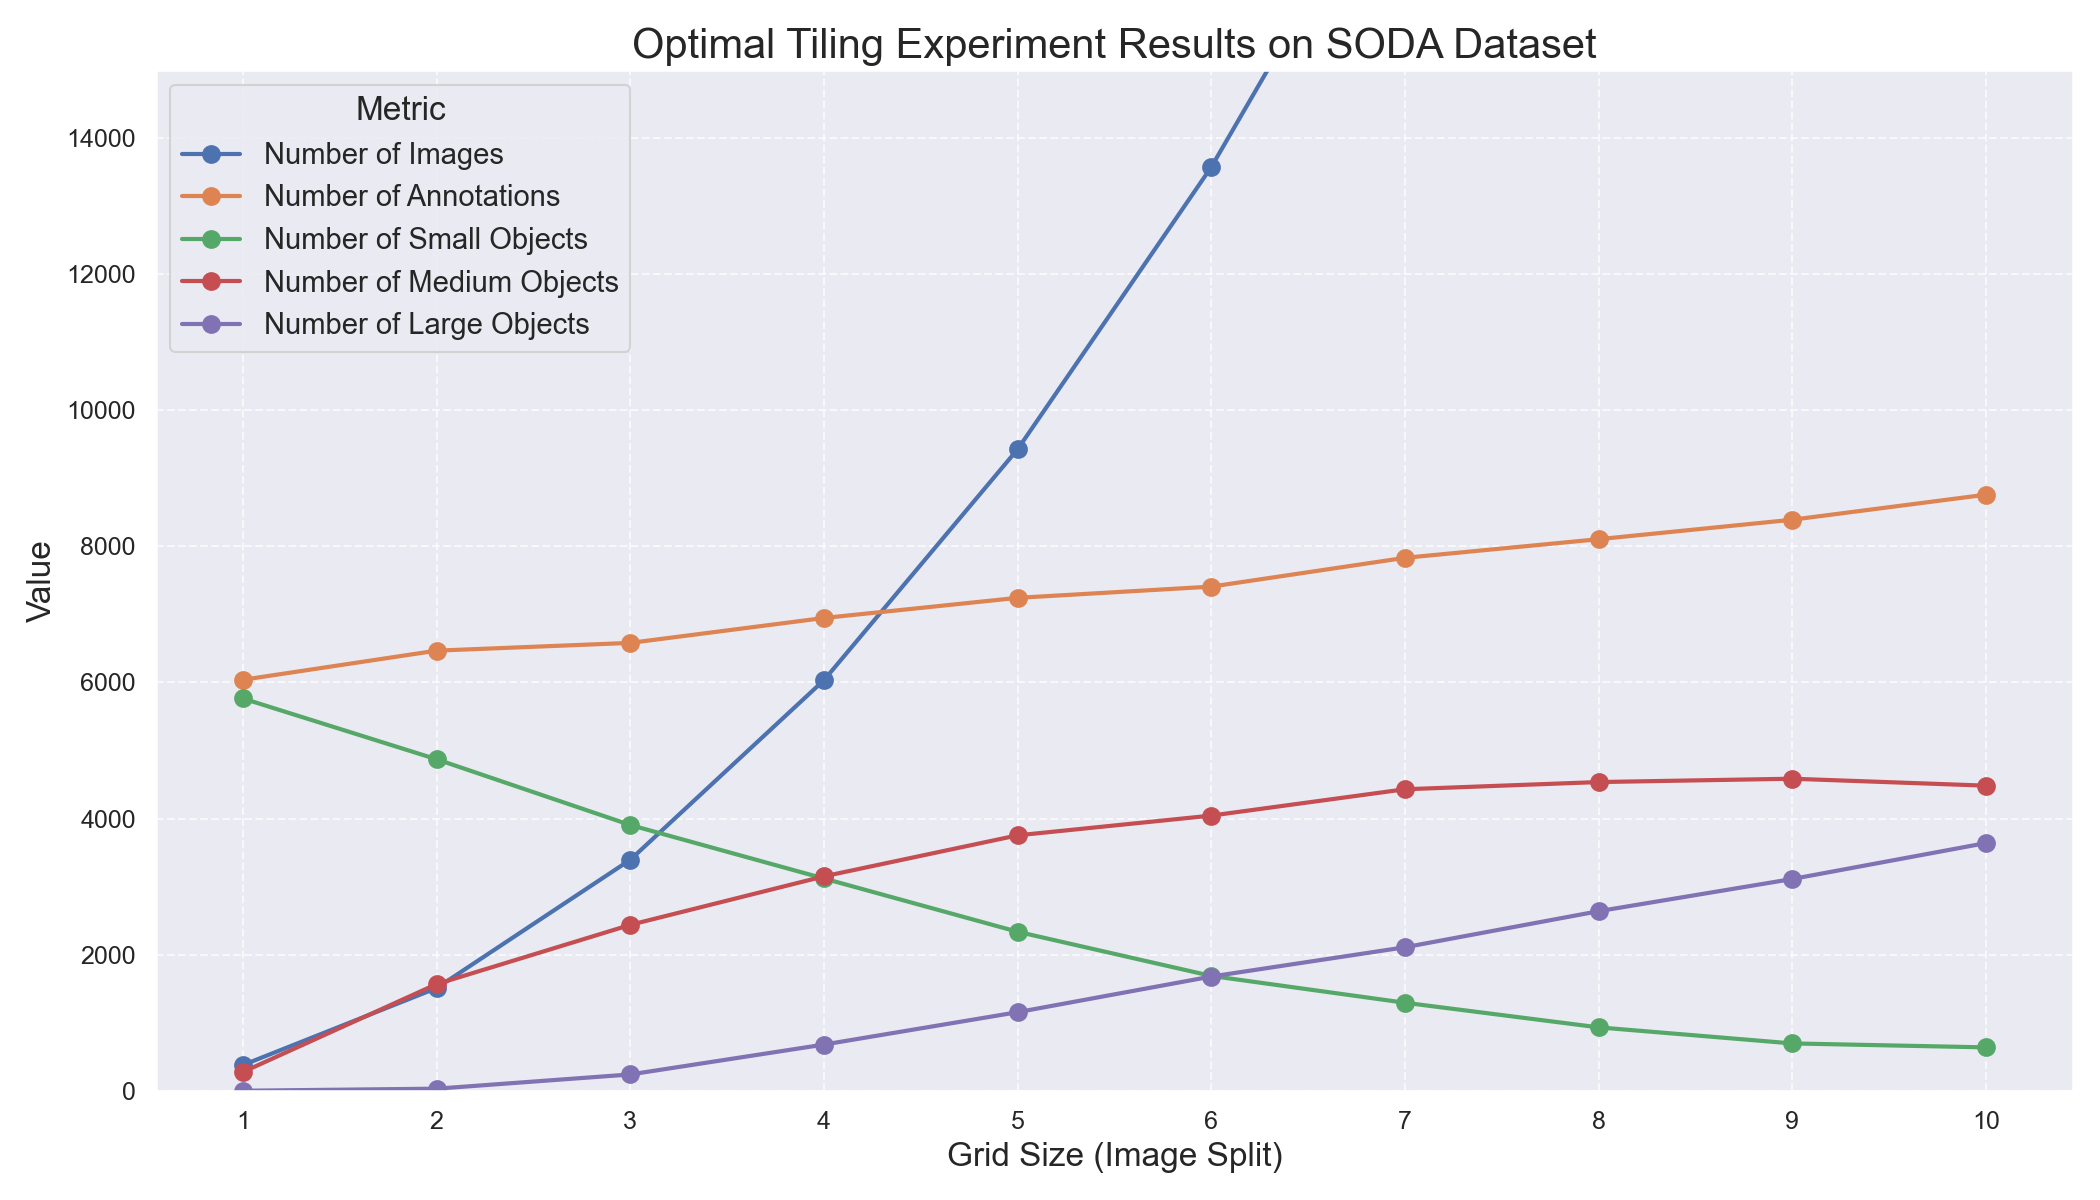
\includegraphics[width=0.9\textwidth]{optimal_tiling_experiment_results_line2.png} \\
    \small (b) \\
  \end{tabular}
  \caption{Optimal tiling experiment results on the \gls{soda} dataset, illustrating the increase in the number of images and annotated objects as the grid size increases. (a) Results over the full altitude range (1--30 metres), and (b) results on a subset of altitudes (5--30 metres) from the \gls{soda} dataset.}
  \label{fig:optimal_tiling_line}
\end{figure}

Two separate experiments were conducted. The first included the full \gls{soda} dataset, covering altitudes from 1 metre to 30 metres. The second considered a subset with altitudes ranging from 5 metres to 30 metres. These configurations were selected to examine whether including very close-range images (such as those at 1 metre) would affect the optimal grid size. The ultimate objective is to develop a single detection model capable of operating effectively across various altitudes. The outcomes of these experiments are illustrated in Figure~\ref{fig:optimal_tiling_line}.

The results of both experiments demonstrate that, as grid size increases, the number of images and annotations also increases. Conversely, the number of small objects decreases, while the count of medium and large objects rises. In the experiment covering all altitudes, the rate of change was more extreme, largely due to the presence of large objects captured at the 1-metre altitude. In contrast, the experiment excluding 1-metre data showed more gradual, consistent changes. Despite this difference, both experiments exhibited the expected trends based on the tiling methodology.
However, these outcomes alone do not provide a direct conclusion regarding the optimal grid size. The goal remains to identify a configuration that reduces the proportion of small objects without introducing excessive computational overhead from processing a high number of tiles. To this end, the ratio of small objects to the number of generated tiles was examined across grid sizes, as shown in Figure \ref{fig:elbow_plot}.

\begin{figure}[!ht]
  \centering
  \begin{tabular}{c}
    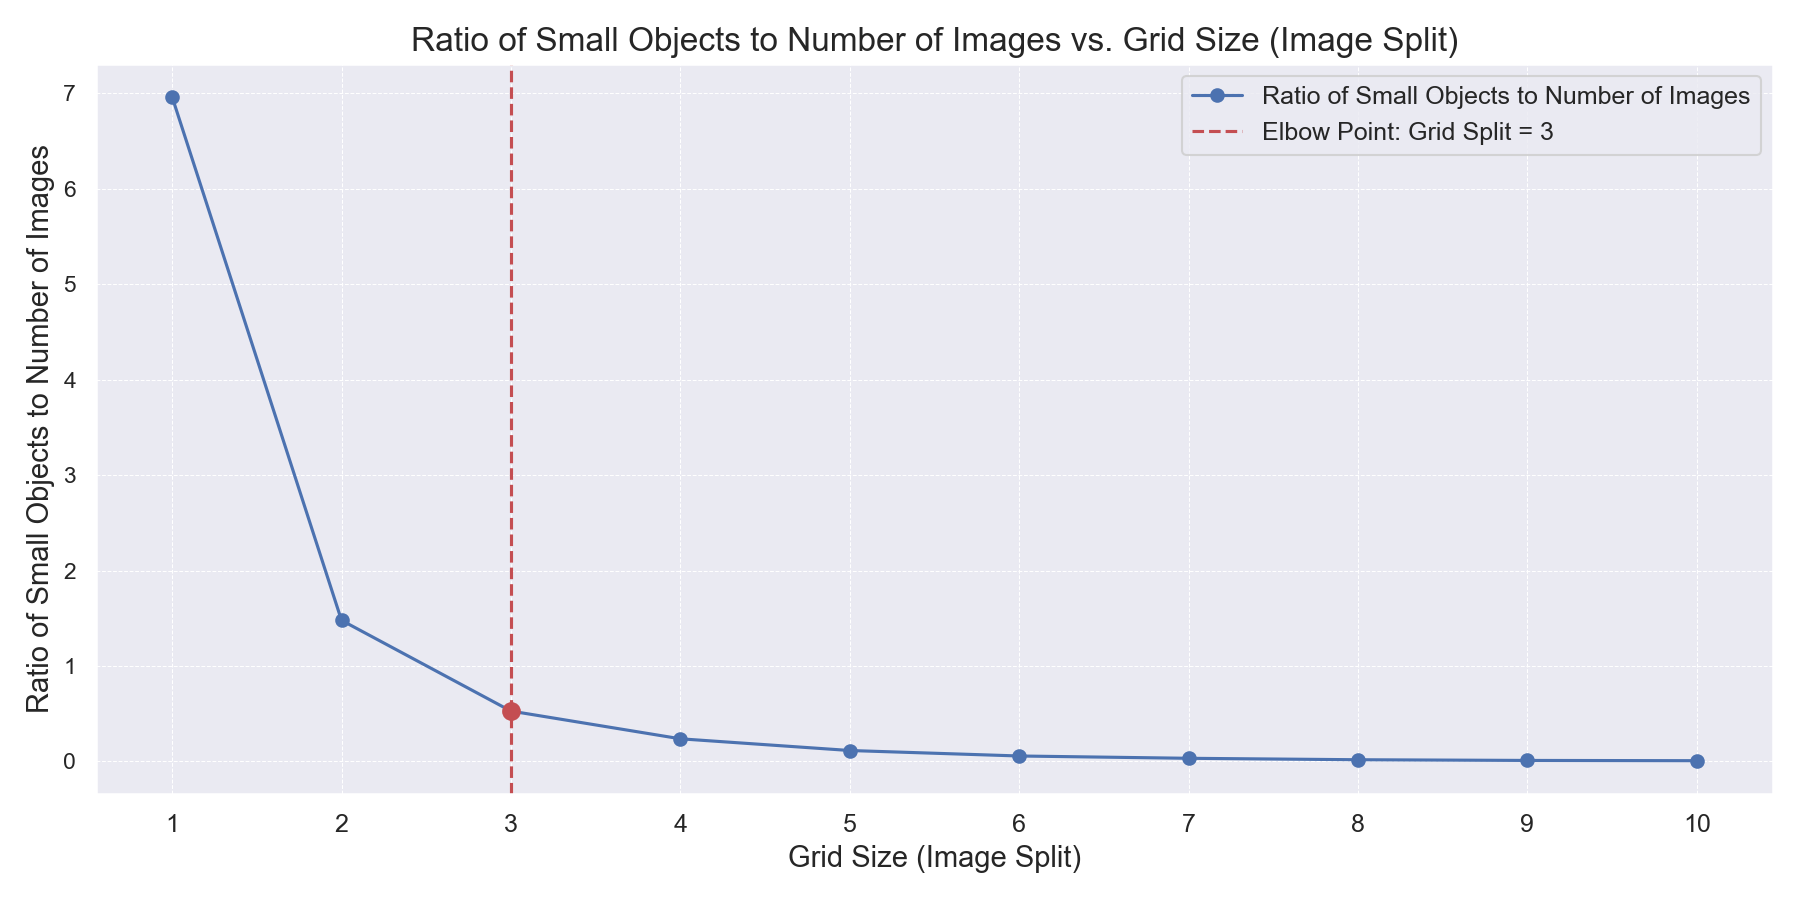
\includegraphics[width=0.9\textwidth]{optimal_tiling_experiment_elbow_method1.png} \\
    \small (a) \\
    \addlinespace[1em]
    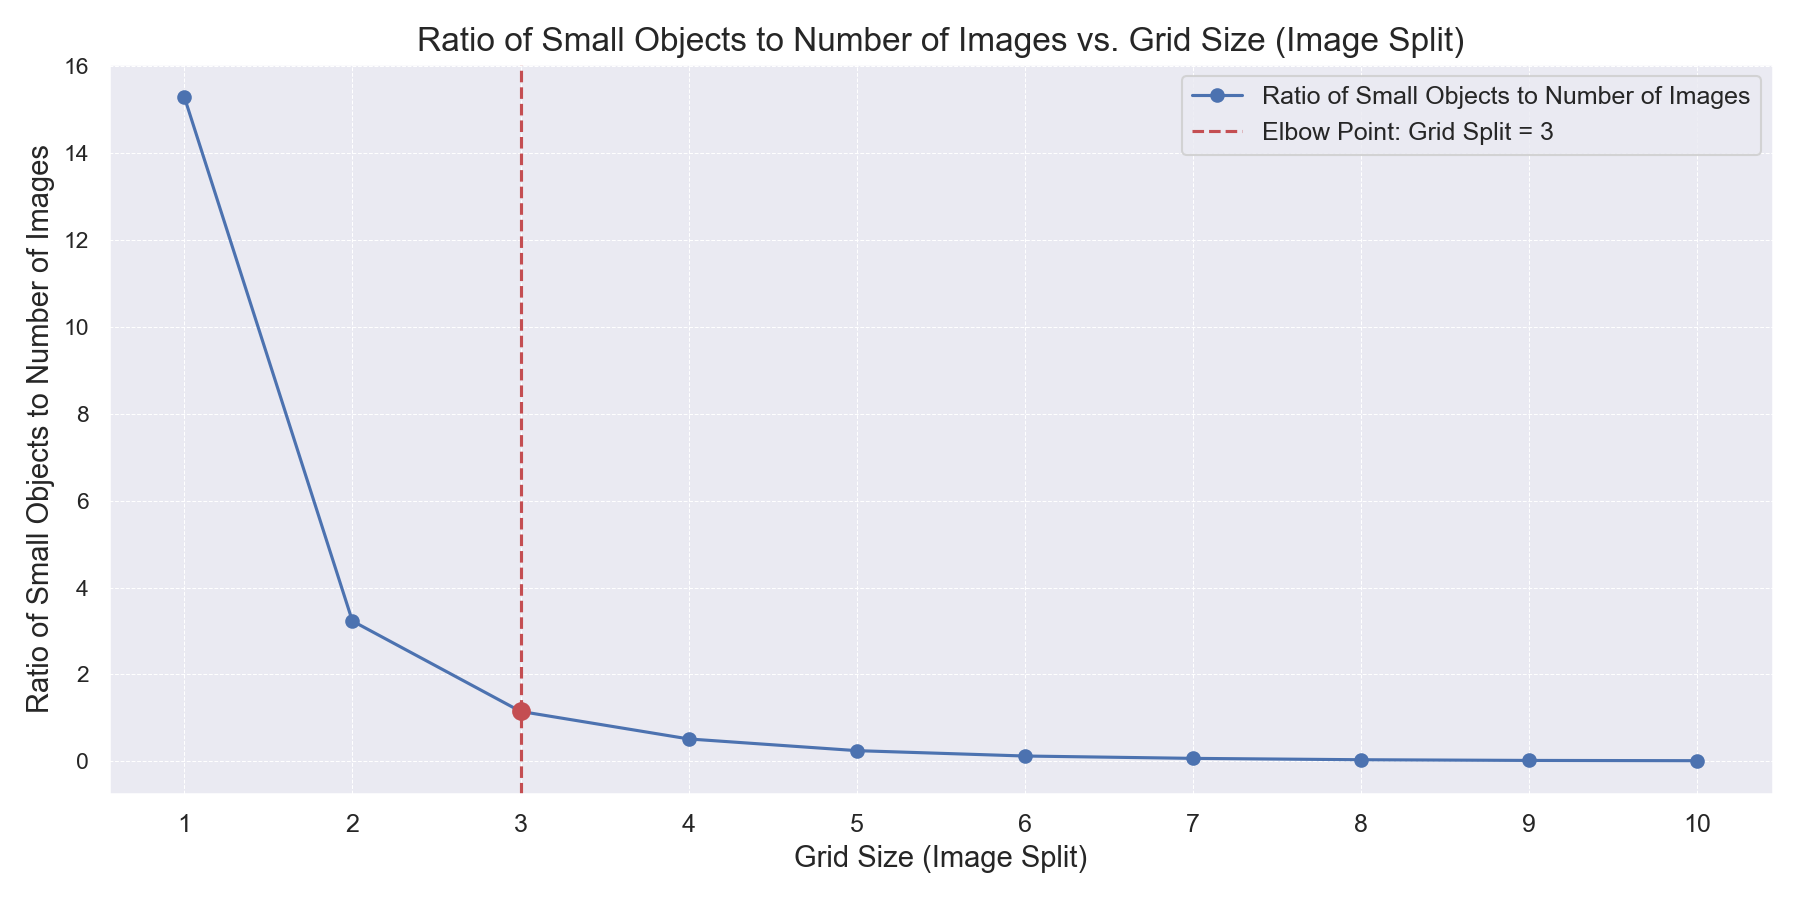
\includegraphics[width=0.9\textwidth]{optimal_tiling_experiment_elbow_method2.png} \\
    \small (b) \\
  \end{tabular}
  \caption{Ratio of small objects to the number of images plotted against tiling grid size, highlighting the observed elbow point in red. (a) Results over the full altitude range (1--30 metres), and (b) results on a subset of altitudes (5--30 metres) from the \gls{soda} dataset.}
  \label{fig:elbow_plot}
\end{figure}

To determine the optimal grid size, the elbow point \cite{elbow_point} method was applied. This approach involved calculating the first and second derivatives of the curve, identifying the point at which the rate of change begins to level off. The second derivative was essential in locating the inflection point, where diminishing returns set in.
Interestingly, both experiments pointed to a 3$\times$3 grid as the optimal configuration. It is worth noting, however, that although the trends across both plots were similar, the ratio of small objects per tile was higher in the all-altitudes experiment. This suggests that including close-range imagery may influence the density of small object annotations.
As a result of this experiment, the tiling configuration used for dataset pre-processing in this study was set to a 3$\times$3 grid for the \gls{soda} dataset (refer to Subsection \ref{subsec:4_soda}), in line with the findings outlined above.

\section{Within-Dataset Evaluation}
\label{sec:5_within_dataset_exp}
% Grazzi Sinjur Alla, Ahfirli Sinjur Alla, u Ismaghni Sinjur Alla. Amen.

% N.B. Visual results and confusion matrix as well, explain different value of alpha, why they were chosen

To assess the proposed integration of the \gls{lupi} paradigm within object detection, litter detection was selected as a case study, supporting the investigation of objectives \textbf{O1}, \textbf{O2}, \textbf{O3}, and partially addressing \textbf{O4}. This task presents a particularly challenging scenario, largely due to the frequent presence of small objects, which considerably complicates the detection process. To examine the effectiveness of the proposed methodology under such conditions, a within-dataset evaluation was conducted using the \gls{soda} dataset.

The \gls{soda} dataset was purposefully chosen as the principal dataset for training \gls{uav}-based litter detection models. Its selection stems from its capacity to represent a diverse range of altitudes and litter types--characteristics not fully captured by the other available \gls{uav}-based litter datasets. The within-dataset evaluation comprised three core experiments: (i) binary litter detection using only the 1-metre altitude subset with no tiling; (ii) binary litter detection on the full \gls{soda} dataset, tiled using a 3$\times$3 grid and covering all altitudes; and (iii) multi-label litter detection using the same 3$\times$3 tiled version across all altitudes. Each of these configurations was chosen for a specific purpose: the first experiment targets detection at close range, the second expands the scope across variable altitudes, and the third introduces additional classification complexity by extending from binary to multi-label tasks, distinguishing between various litter types and the background.

For each of these experiments, the five object detection architectures detailed in Section \ref{sec:4_distillation_architectures} were trained: Faster \gls{rcnn}, \gls{ssd}, RetinaNet, SSDLite, and \gls{fcos}. For each architecture, a baseline model, a teacher model, and four student models were trained with varying levels of teacher guidance. Consequently, 30 distinct models were trained for each experiment.

The central objective was to determine whether student models trained using the \gls{lupi} framework, with access to privileged training signals, could outperform their respective baselines, which were trained using only standard input data. For each architecture, a teacher model was first trained, followed by the training of student models using five distinct \gls{alpha} values: 0, 0.25, 0.5, 0.75, and 1. These values match those used in related work in \gls{lupi} \cite{lab2wild}. An $\alpha$ of 0 represents the baseline, where the student is trained without any guidance from the teacher, while $\alpha = 1$ reflects full reliance on the teacher’s output during training. The intermediate values allowed a controlled study of how varying degrees of teacher influence affected model performance.


Importantly, this study did not involve cross-architecture distillation. In other words, teacher models were used only to train student models of the same architecture. This approach was adopted to avoid the added complexity of aligning latent feature representations between different model types, which would have required additional mechanisms and exceeded the scope of this work.

All models were trained using the designated training subsets, while validation and testing were carried out on their respective set partitions. The evaluation employed the detection metrics outlined in Section \ref{sec:4_metrics}, providing a consistent and coherent basis for comparison. A uniform pre-processing pipeline and identical training configurations were applied across all models, ensuring fairness in evaluation. Given this diverse range of detection architectures and the controlled experimental setup, the resulting outcomes offer a reliable and concrete basis for assessing the influence of \gls{lupi} in object detection.


\subsection{Binary Litter Detection on the SODA Dataset at 1-Metre Altitude}
\label{subsec:5_soda01m_dataset_exp}
% Glorja lil Missier lil Iben u lil Ispirtu s-Santu, Grazzi. Amen

The first experiment aimed to assess the benefits of using the \gls{lupi} framework for close-range litter detection. To this end, a subset of the \gls{soda} dataset at a 1-metre altitude was selected, consisting of 452 images. These images were divided into 316 for training, 46 for validation, and 90 for testing. In this experiment, detection models were trained to classify all litter into a single category, distinguishing between litter (foreground) and background.

The results of this experiment, comparing the baseline model with the best student model across all five selected detection architectures, are presented in Figure \ref{fig:soda01m_bar}. In all architectures, the student model outperformed the baseline, showing a notable improvement in detection accuracy, particularly in the challenging \gls{map}@50–95 metric. Additionally, improvements were seen in other key detection metrics, including precision, recall, and F1 score. Among the models, the RetinaNet student achieved the highest performance, followed by the Faster \gls{rcnn} and \gls{fcos} student models. Across all metrics, the student models demonstrated an accuracy improvement ranging from 0.05 to 0.15. Interestingly, when comparing the baseline models with the student models, RetinaNet and \gls{ssd} showed the highest improvements in detection accuracy, with the student models outperforming their baseline counterparts. The other architecture types, such as Faster \gls{rcnn} and \gls{fcos}, also saw improvements, though the performance boosts were somewhat smaller in comparison to those of RetinaNet and \gls{ssd}.

\begin{figure}[!ht]
    \centering
    \includegraphics[width=1\textwidth]{SODA 01m Dataset (Single-label).png}
    \caption{Comparison between the baseline and the best-performing student models across key detection metrics on the \gls{soda} dataset at a 1-metre altitude for binary litter detection.}
    \label{fig:soda01m_bar}
\end{figure}

While RetinaNet, \gls{fcos}, and Faster \gls{rcnn} delivered the best results in this experiment, which can be attributed largely to their complex architectures and the use of the ResNet-\gls{fpn} backbone, notable improvements were also observed with the \gls{ssd} and SSDLite architectures. This suggests that the \gls{lupi} method can improve litter detection performance at close range, even in complex environments with backgrounds such as rocks and plants. The results indicate that, regardless of the architecture, \gls{lupi} significantly improves detection accuracy in close-range binary detection.

In addition to the comparison between the baseline and student models, a further analysis was conducted to evaluate the performance of the different teacher models, using the same evaluation metrics and experimental setup. The results are summarised in Table~\ref{tab:teacher_model_metrics_soda01m}, which presents the detection accuracy achieved by each teacher model architecture. It can be observed that Faster \gls{rcnn}, \gls{fcos}, and RetinaNet stood out as the highest-performing teacher models. Most of their detection metrics approached 1.0, suggesting near-ideal detection performance across the evaluated scenes. 
% These results highlight the informative nature of these teacher networks, especially in supporting the \gls{lupi} training paradigm.

\begin{table}[!ht]
    \centering
    \begin{adjustbox}{max width=\textwidth}
    \renewcommand{\arraystretch}{1.5}
    \begin{tabular}{|l|c|c|c|c|c|c|c|c|c|}
        \hline%\toprule
        \textbf{Model} & \textbf{mAP@50--95} & \textbf{mAP@50} & \textbf{mAP@75} & \textbf{mAR@1} & \textbf{mAR@10} & \textbf{mAR@100} & \textbf{Precision} & \textbf{Recall} & \textbf{F1 Score} \\ \hline \hline
        \textbf{RetinaNet} & 0.94 & 0.98 & 0.96 & 0.63 & 0.96 & 0.96 & 0.93 & 0.99 & 0.96 \\\hline
        \textbf{FCOS} & \textbf{0.96} & 0.98 & 0.97 & 0.63 & 0.97 & 0.97 & 0.81 & 0.99 & 0.89 \\\hline
        \textbf{Faster R-CNN} & \textbf{0.96} & \textbf{0.99} & \textbf{0.98} & \textbf{0.63} & \textbf{0.98} & \textbf{0.98} & \textbf{0.99} & \textbf{0.99} & \textbf{0.99} \\\hline
        \textbf{SSD} & 0.78 & 0.96 & 0.94 & 0.54 & 0.81 & 0.81 & 0.65 & 0.99 & 0.79 \\\hline
        \textbf{SSDLite} & 0.61 & 0.73 & 0.72 & 0.48 & 0.63 & 0.63 & 0.02 & 0.99 & 0.03 \\
        \hline%\bottomrule
    \end{tabular}
    \renewcommand{\arraystretch}{1}
    \end{adjustbox}
    \caption{Comparison of teacher model performance across key detection metrics, trained on the \gls{soda} dataset at a 1-metre altitude for binary litter detection.}
    \label{tab:teacher_model_metrics_soda01m}
\end{table}

On the other hand, the \gls{ssd} and SSDLite teacher models, while still achieving reasonable scores, demonstrated noticeably lower accuracy. Even when trained with privileged information, these architectures did not attain the same level of conceptual understanding, indicating limitations in adapting to this particular detection task. Combined with the student model results in Figure~\ref{fig:soda01m_bar}, this suggests that these architectures may be less suited to scenarios requiring high sensitivity to fine-grained object features.

Interestingly, while Faster \gls{rcnn} proved to be the top-performing teacher model, it was not associated with the best-performing student. That distinction went to the RetinaNet student model. Given that both architectures share a similar ResNet-\gls{fpn} backbone and were distilled at equivalent feature extraction layers, this outcome suggests that RetinaNet may be structurally more compatible with learning using privileged information in this context.
Across all teacher models, recall was generally high, while precision tended to be lower. This implies that the teacher models were primarily geared toward minimising \gls{fn}.
% , reinforcing their utility in guiding student models to identify more instances, albeit sometimes at the expense of \gls{fp}.

While the results clearly show that \gls{lupi} improves detection accuracy in this particular experiment, it is also important to acknowledge that this improvement does not come without cost. Training within the \gls{lupi} framework requires an additional training phase, wherein a teacher model must be trained before the student. Moreover, each model must process privileged inputs during training, resulting in larger tensors and increased computational demands, despite only minor adjustments to the teacher architecture and none to the student.

To examine the impact of these changes on training duration, Figure~\ref{fig:soda01m_training_time} presents a comparison of training times across all models involved in this experiment. As shown in the figure, both student and teacher models required substantially more time to train than the baseline models. This increase is due in part to the two-stage nature of the training process and, for student models specifically, the added computation needed to process the teacher’s outputs and compute the distillation loss. The time taken by the teacher during inference directly contributes to the student’s overall training time.

\begin{figure}[!ht]
    \centering
    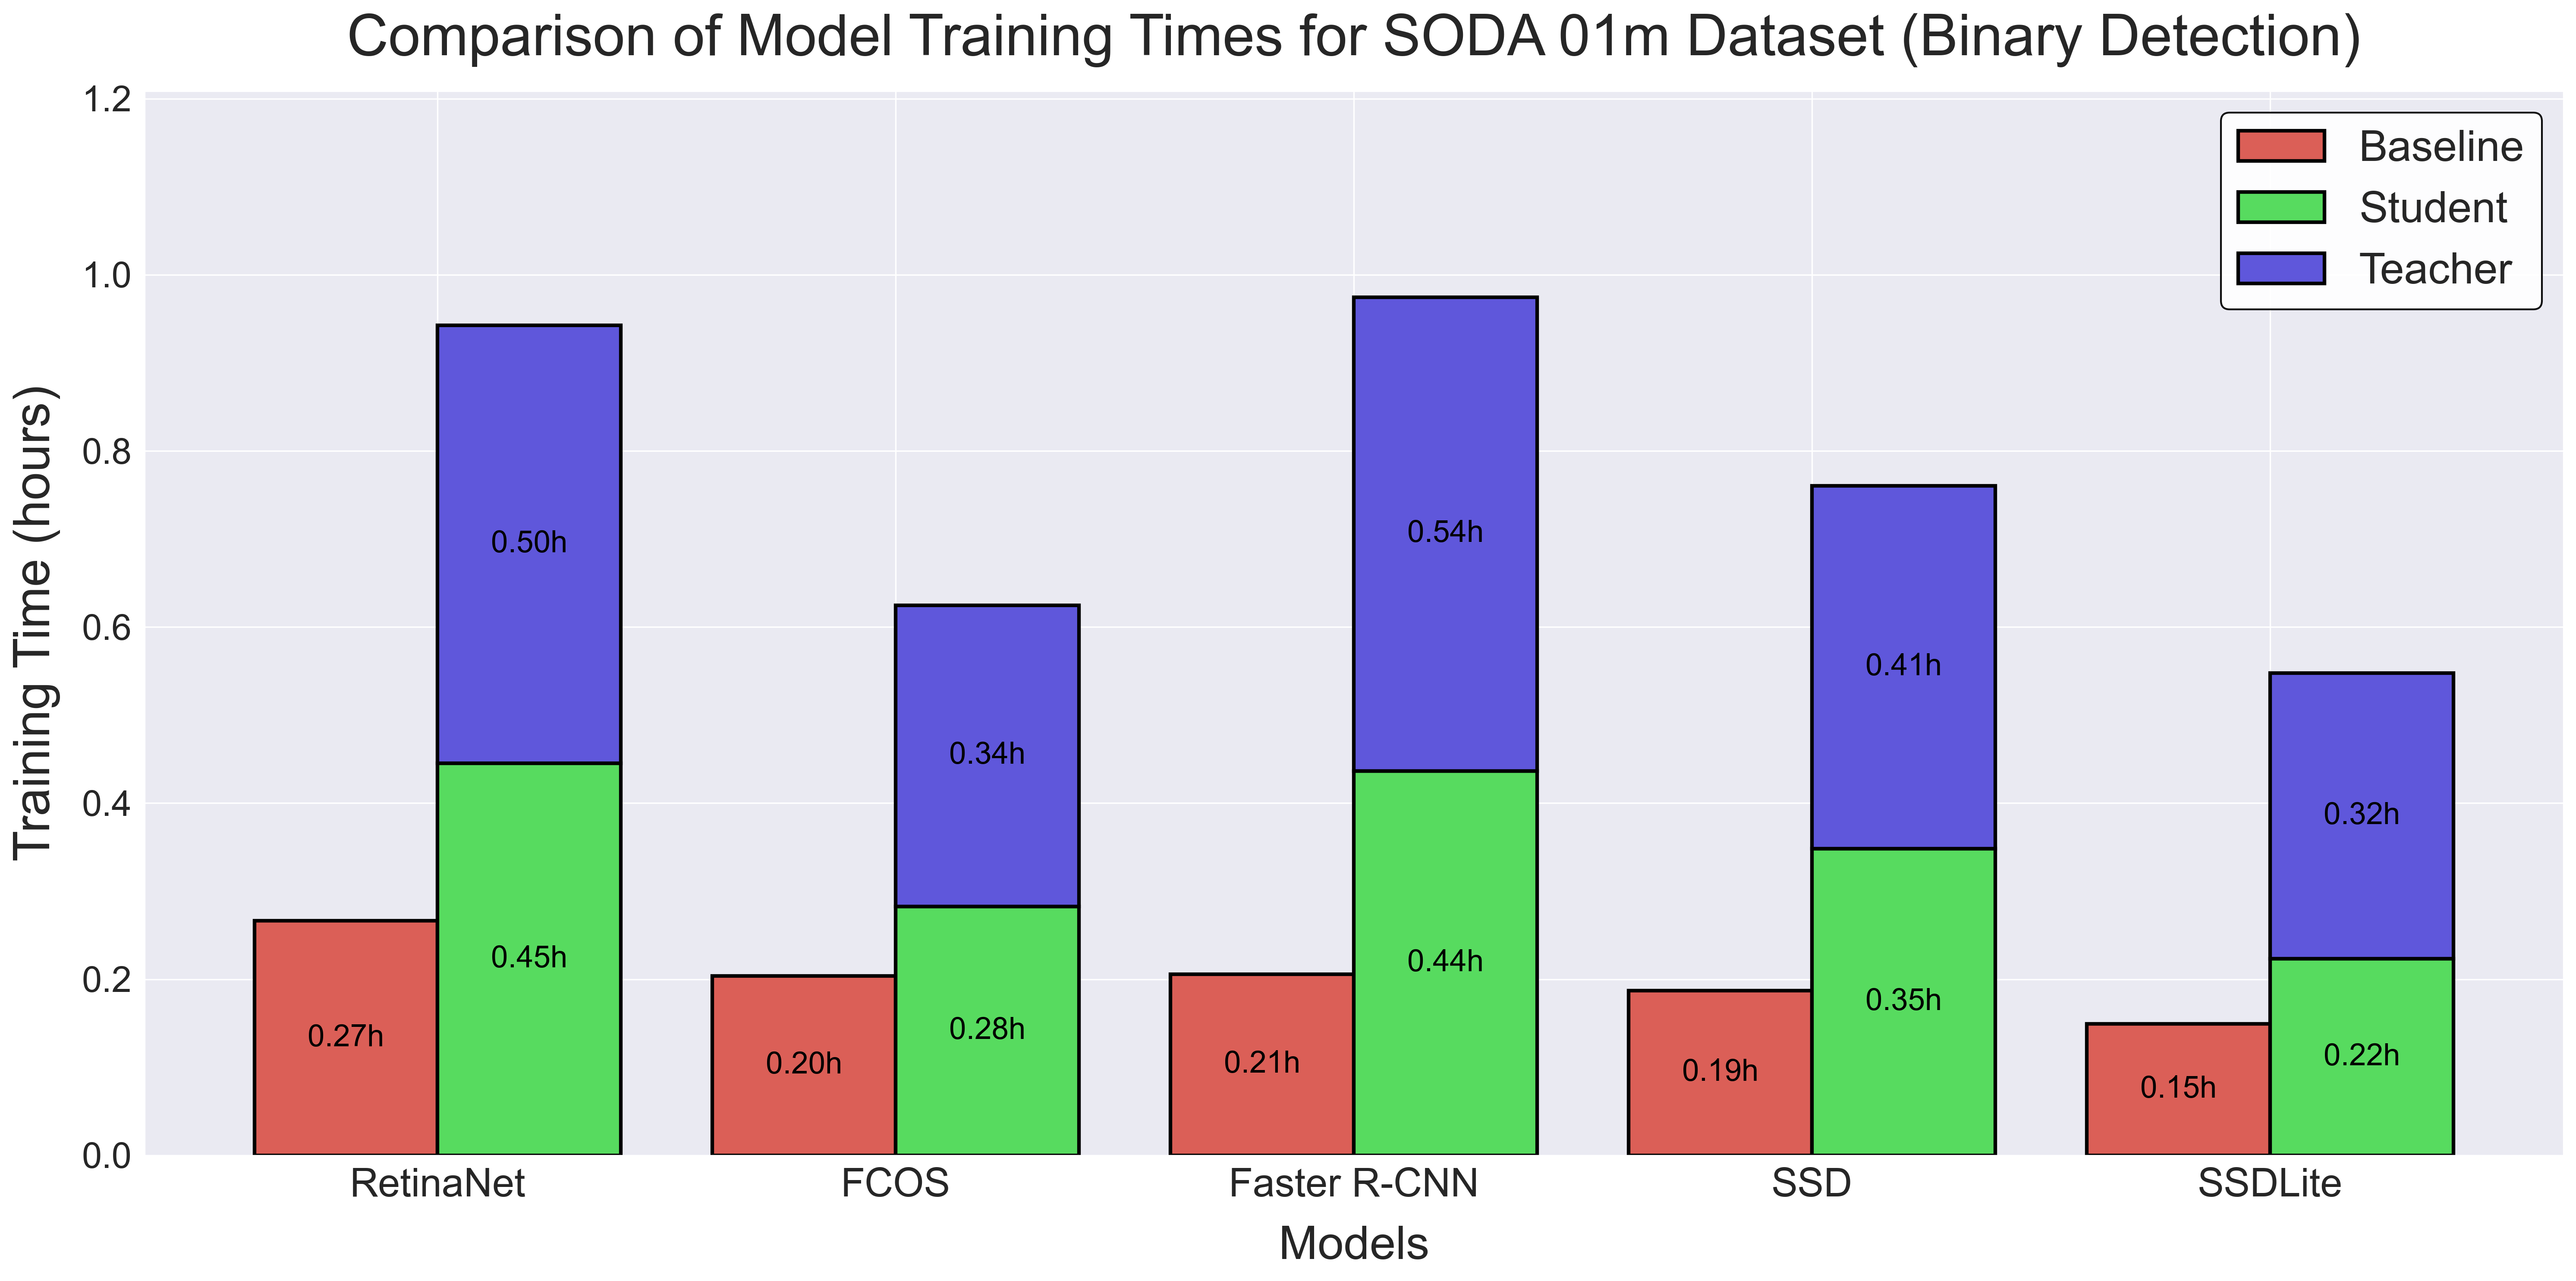
\includegraphics[width=1\textwidth]{training_times_soda_01m_dataset_binary_detection.png}
    \caption{Comparison of model training times on the \gls{soda} dataset at a 1-metre altitude for binary litter detection.}
    \label{fig:soda01m_training_time}
\end{figure}

In terms of model-specific performance, \gls{fcos} and SSDLite exhibited the shortest training durations, whereas RetinaNet and Faster \gls{rcnn} incurred the highest training times, especially under the \gls{lupi} setup. Notably, teacher models consistently recorded the longest training durations across all architectures.

Despite the increase in training time, a comparison of model size and parameter count between the baseline and student models, as shown in Table~\ref{tab:model_configs_soda01m}, shows that they remain identical across all architectures. This suggests that student models benefit from improved detection accuracy through \gls{lupi} without adding any cost in terms of model size or computational demands during inference. In contrast to many modern detection models that require larger storage and are computationally intensive at deployment \cite{detr, rt-detr, rt-detrv2, rf-detr}, the student models preserve the compactness of their baseline versions.

\begin{table}[!ht]
    \centering
    \begin{tabular}{llcc}
        \toprule
        \textbf{Model Configuration} & \textbf{Type} & \textbf{Size (MB)} & \textbf{Parameters (M)} \\
        \midrule
        \multirow{5}{*}{\textbf{Baseline}} 
            & RetinaNet   & 122.72 & 32.17 \\
            & FCOS        & 122.32 & 32.06 \\
            & Faster R-CNN & 157.54 & 41.30 \\
            & SSD         & 90.58  & 23.75 \\
            & SSDLite     & 8.42   & 2.21 \\
        \midrule
        \multirow{5}{*}{\textbf{Student}} 
            & RetinaNet   & 122.72 & 32.17 \\
            & FCOS        & 122.32 & 32.06 \\
            & Faster R-CNN & 157.54 & 41.30 \\
            & SSD         & 90.58  & 23.75 \\
            & SSDLite     & 8.42   & 2.21 \\
        \bottomrule
    \end{tabular}
    \caption{Comparison of model configurations for trained baseline and student models on the \gls{soda} dataset at a 1-metre altitude for binary litter detection, including model type, size in megabytes, and number of parameters (in millions).}
    \label{tab:model_configs_soda01m}
\end{table}

It is also important to point out that Faster \gls{rcnn}, \gls{fcos}, and RetinaNet occupy more memory overall, as they rely on larger architectural designs. On the other hand, \gls{ssd} and SSDLite remain comparatively lightweight. Even so, the main observation remains clear. In the context of \gls{uav}-based binary litter detection, where lightweight architectures are essential due to hardware limitations, \gls{lupi} enables improved detection accuracy without increasing model size. This makes it a practical solution for situations where both storage and computational efficiency are important.

\subsection{Binary Litter Detection on the SODA Dataset Across All Altitudes}
\label{subsec:5_soda_tiled_single_dataset_exp}
% Glorja lil Missier, lil Iben u lil Ispirtu s-Santu. Amen

The second experiment aimed to build upon the context of the first by further exploring the benefits of using the \gls{lupi} framework for litter detection at higher altitudes, addressing the challenges posed by more complex detection scenarios. To this end, the entire \gls{soda} dataset was tiled in a 3$\times$3 configuration at all altitudes to reflect a more complex, real-world scenario for \gls{uav}-based litter detection. This dataset included 7,461 images, with 5,238 allocated for training, 765 for validation, and 1,458 for testing. In this experiment, detection models were trained to classify all litter into a single category, focusing on distinguishing small litter from variable and challenging backgrounds.

The results of this experiment, comparing the baseline model with the best-performing student model across all five selected detection architectures, are presented in Figure~\ref{fig:soda_tiled_single_bar}. In most cases, the student models performed better than their baseline counterparts, showing noticeable improvements in detection accuracy, particularly in the more demanding \gls{map}@50–95 metric. In addition, improvements were also observed in precision, recall, and F1 score metrics. However, the \gls{ssd} and SSDLite architectures exhibited little to no improvement.
Compared to the earlier experiment shown in Figure~\ref{fig:soda01m_bar}, the results here reflect a tougher detection setting, which generally led to lower overall performance. Even so, models trained with the \gls{lupi} framework still showed clear advantages. 

\begin{figure}[!ht]
    \centering
    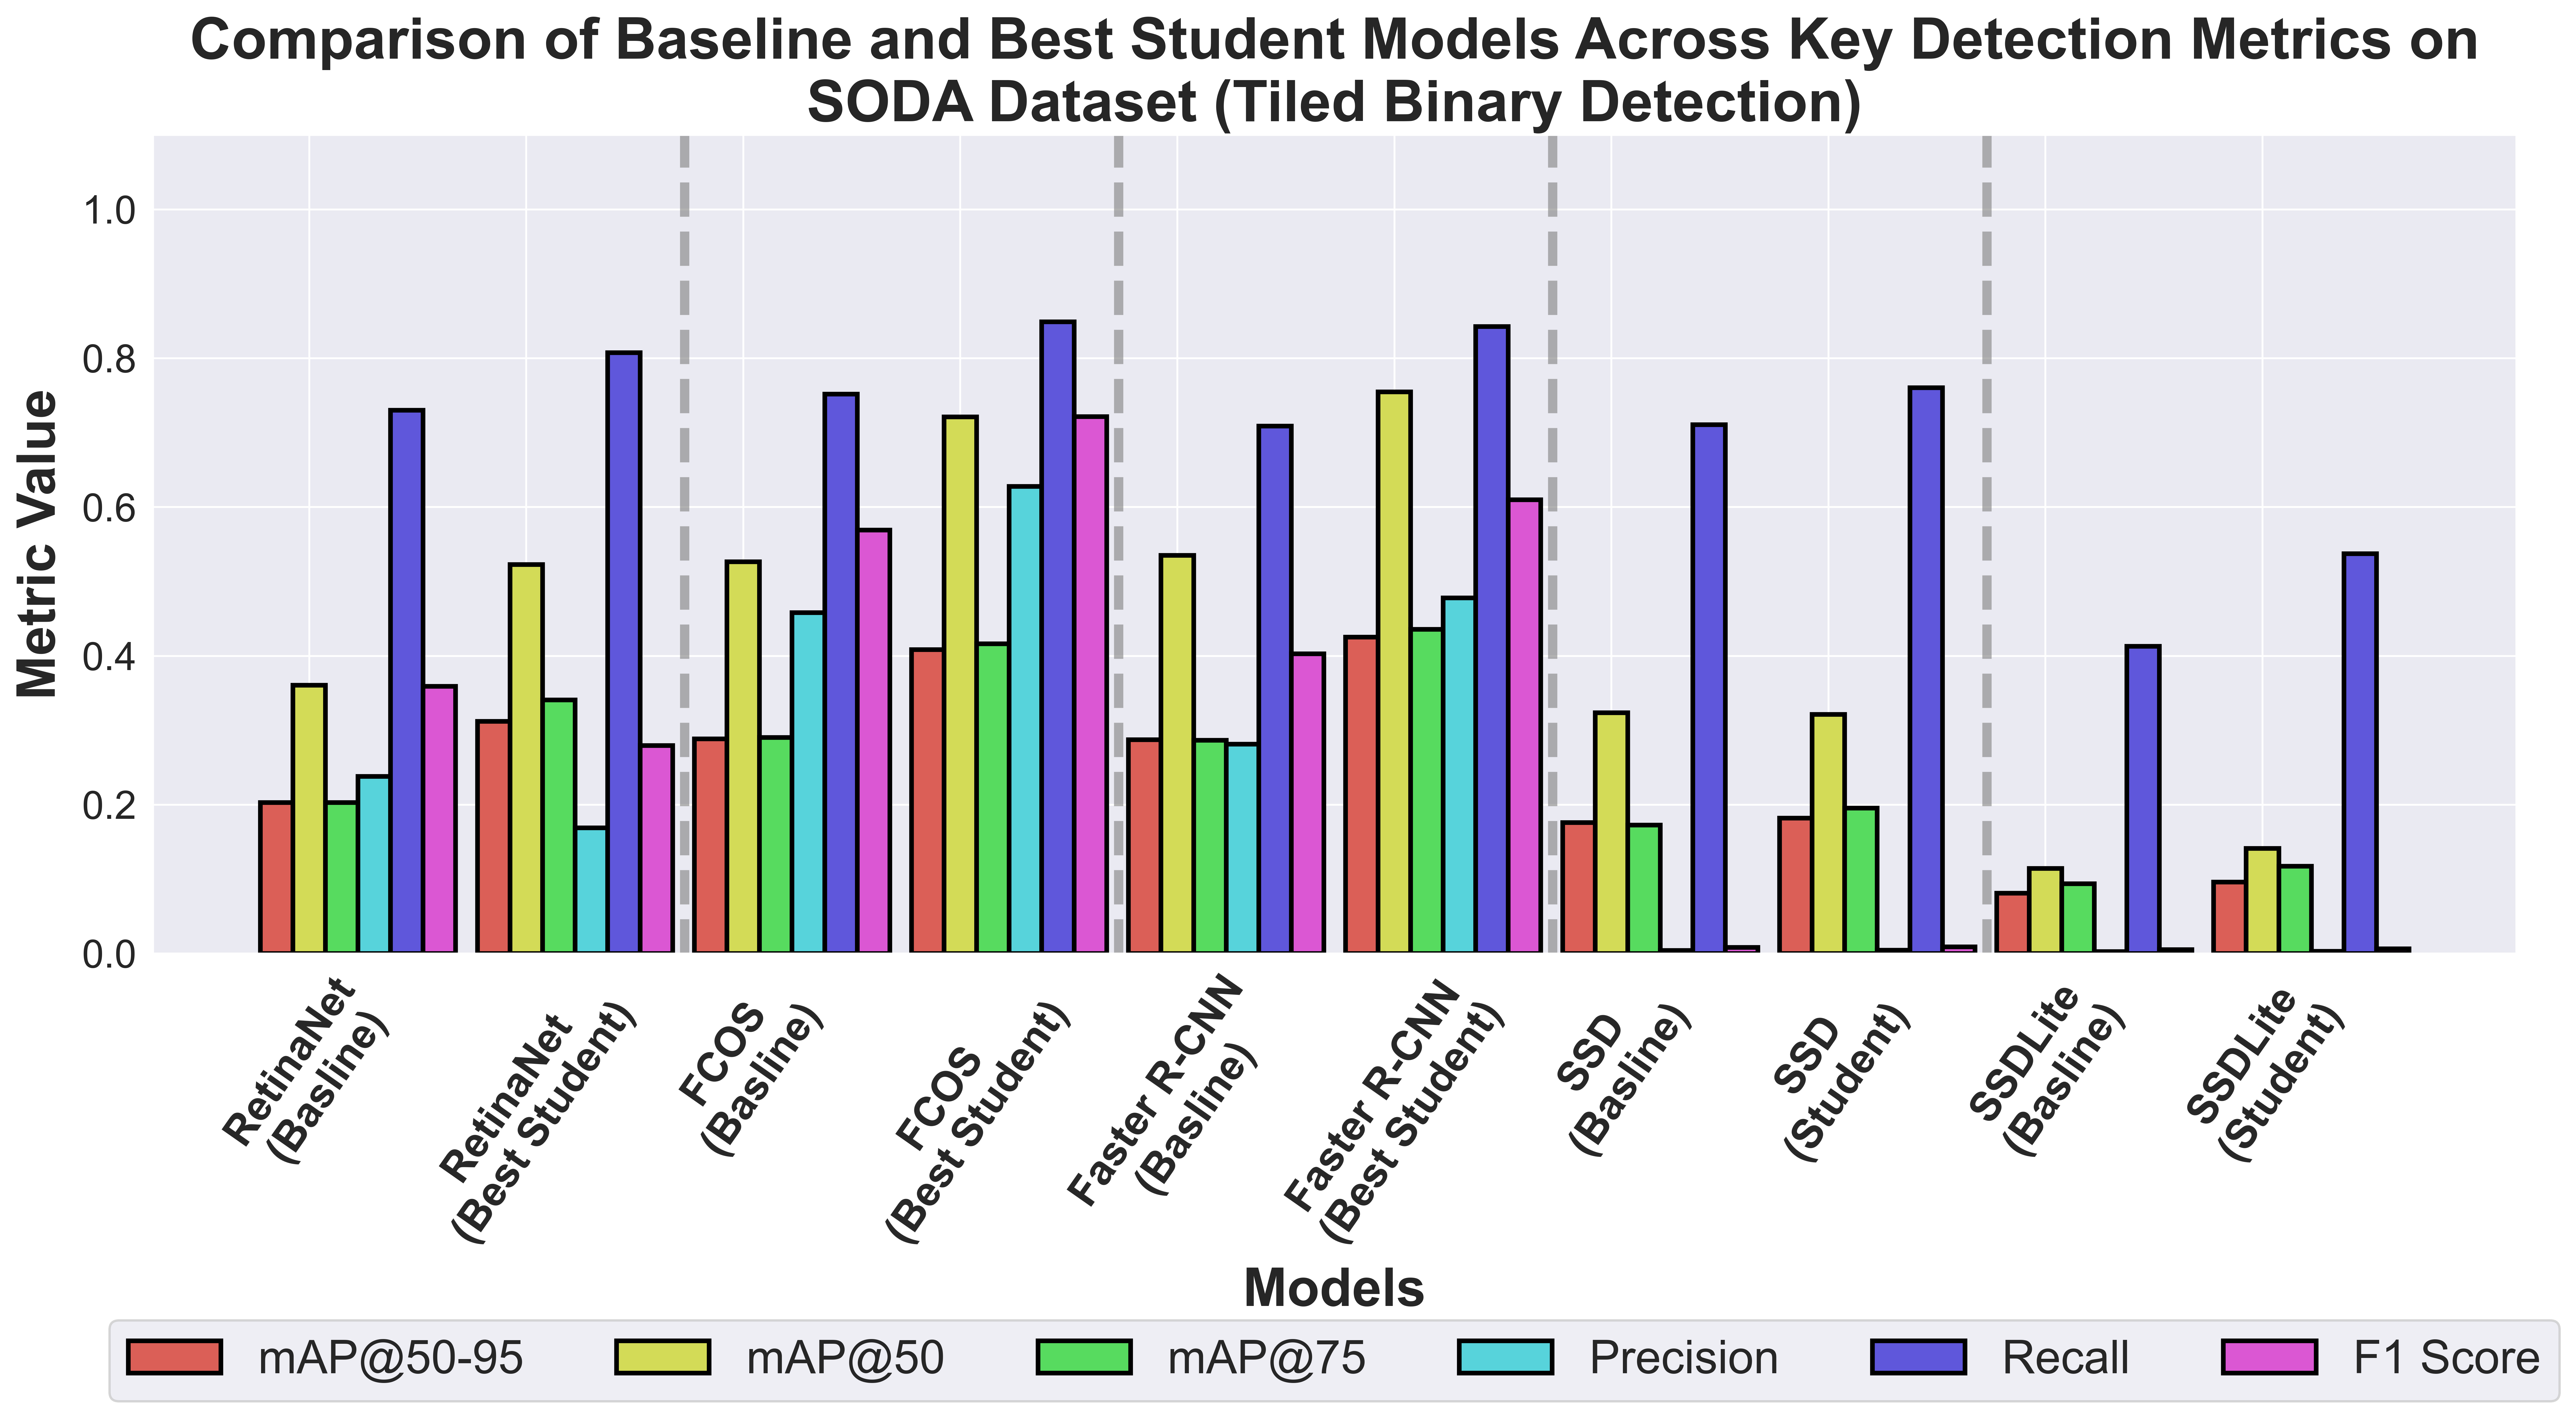
\includegraphics[width=1\textwidth]{SODA Dataset (Tiled Binary Detection).png}
    \caption{Comparison between the baseline and best-performing student models across key detection metrics on the 3$\times$3 tiled \gls{soda} dataset across all altitudes for binary litter detection.}
    \label{fig:soda_tiled_single_bar}
\end{figure}

Among all models, the student version of Faster \gls{rcnn} delivered the best overall results, followed by \gls{fcos} and RetinaNet. This marks a shift from the previous experiment, where RetinaNet had achieved the highest scores. The performance of Faster \gls{rcnn} suggests that its two-stage architecture may be better suited to the demands of this task than the one-stage approaches. Furthermore, the student models outperformed their baseline counterparts across all evaluated metrics, with accuracy improvements ranging from 0.01 to 0.11. \gls{fcos} and Faster \gls{rcnn} recorded the most noticeable performance boosts compared to their baselines. RetinaNet and SSDLite also benefitted, though to a lesser degree. For \gls{ssd}, the improvement was limited, appearing only in the \gls{map}@75 metric.

Moreover, the findings further support the selection of Faster \gls{rcnn}, \gls{fcos}, and RetinaNet as more effective detection architectures in this context, especially when compared to the lighter alternatives, owing to their structural complexity and performance consistency.
In addition to this comparison, a further analysis was carried out to assess the efficacy of different teacher models, following a similar approach to the previous experiment. The outcomes, presented in Table~\ref{tab:teacher_model_metrics_soda_tiled_single}, detail the detection accuracy attained by each teacher architecture. Once again, Faster \gls{rcnn}, \gls{fcos}, and RetinaNet emerged as the top performers, with several of their metrics approaching ideal values, though with slight reductions in some areas. These results indicate that, despite the increased scene complexity, these models continue to demonstrate high detection accuracy.

\begin{table}[!ht]
    \centering
    \begin{adjustbox}{max width=\textwidth}
    \renewcommand{\arraystretch}{1.5}
    \begin{tabular}{|l|c|c|c|c|c|c|c|c|c|}
        \hline
        \textbf{Model} & \textbf{mAP@50--95} & \textbf{mAP@50} & \textbf{mAP@75} & \textbf{mAR@1} & \textbf{mAR@10} & \textbf{mAR@100} & \textbf{Precision} & \textbf{Recall} & \textbf{F1 Score} \\ \hline \hline
        \textbf{RetinaNet} & 0.90 & 0.95 & 0.94 & 0.34 & 0.83 & 0.91 & 0.41 & 0.98 & 0.58 \\\hline
        \textbf{FCOS} & 0.89 & 0.94 & 0.93 & 0.34 & 0.82 & 0.90 & \textbf{0.97} & 0.96 & 0.96 \\\hline
        \textbf{Faster R-CNN} & \textbf{0.96} & \textbf{0.99} & \textbf{0.98} & \textbf{0.35} & \textbf{0.87} & \textbf{0.97} & 0.96 & \textbf{0.99} & \textbf{0.98} \\\hline
        \textbf{SSD} & 0.49 & 0.62 & 0.59 & 0.27 & 0.51 & 0.51 & 0.16 & 0.97 & 0.27 \\\hline
        \textbf{SSDLite} & 0.18 & 0.23 & 0.19 & 0.17 & 0.19 & 0.19 & 0.00 & 0.79 & 0.01 \\
        \hline
    \end{tabular}
    \renewcommand{\arraystretch}{1}
    \end{adjustbox}
    \caption{Comparison of teacher model performance across key detection metrics, trained on the 3$\times$3 tiled \gls{soda} dataset across all altitudes for binary litter detection.}
    \label{tab:teacher_model_metrics_soda_tiled_single}
\end{table}

The \gls{ssd} and SSDLite teacher models, while producing acceptable results, exhibited a noticeable decline in detection accuracy relative to the other models. This drop was particularly evident when assessing performance through \gls{map} and F1 score. Moreover, their results showed a significant reduction compared to the first experiment, further emphasising the limitations in their ability to generalise, particularly given the added complexity introduced by small object detection.

In contrast to the first experiment conducted at 1 metre altitude, Faster \gls{rcnn} emerged as the most effective teacher and student model in this multi-altitude experiment. RetinaNet, which incorporates focal loss to address class imbalance between foreground and background, underperformed relative to both Faster \gls{rcnn} and \gls{fcos}, with some detection metrics showing a gap of 0.1 or more in terms of the models outlined in Figure \ref{fig:soda_tiled_single_bar}. This suggests that RetinaNet may not be ideally suited for detecting litter in scenes characterised by visually complex and variable backgrounds. \gls{fcos}, leveraging \textit{centre-ness} loss to improve spatial accuracy, delivered results on par with Faster \gls{rcnn} across both baseline and student models, reinforcing its reliability under these conditions.

Notably, the consistent use of the ResNet-\gls{fpn} backbone across Faster \gls{rcnn}, \gls{fcos}, and RetinaNet likely contributed to their relative success. The \gls{fpn}’s capacity for multi-scale object detection aligns well with the demands of \gls{uav}-based litter detection at varying altitudes. This architectural feature appears to bolster compatibility with learning via privileged information.

Across the teacher models, recall remained consistently high, while precision tended to be lower. Once again, this suggests that the models were primarily geared toward reducing \gls{fn}, which is generally beneficial in domains where missing detections is costly. However, in the context of litter detection, this emphasis may be less appropriate, as an increase in \gls{fp} can also undermine model reliability.

The training durations for all models employed in this experiment are presented in Figure~\ref{fig:soda_tiled_single_training_time}. The outcomes differ slightly from those of the first experiment (refer to Figure~\ref{fig:soda01m_training_time}). In certain instances, the student model required marginally less time to train than its baseline counterpart, though this difference was observed solely in the case of RetinaNet and was negligible.

\begin{figure}[!ht]
    \centering
    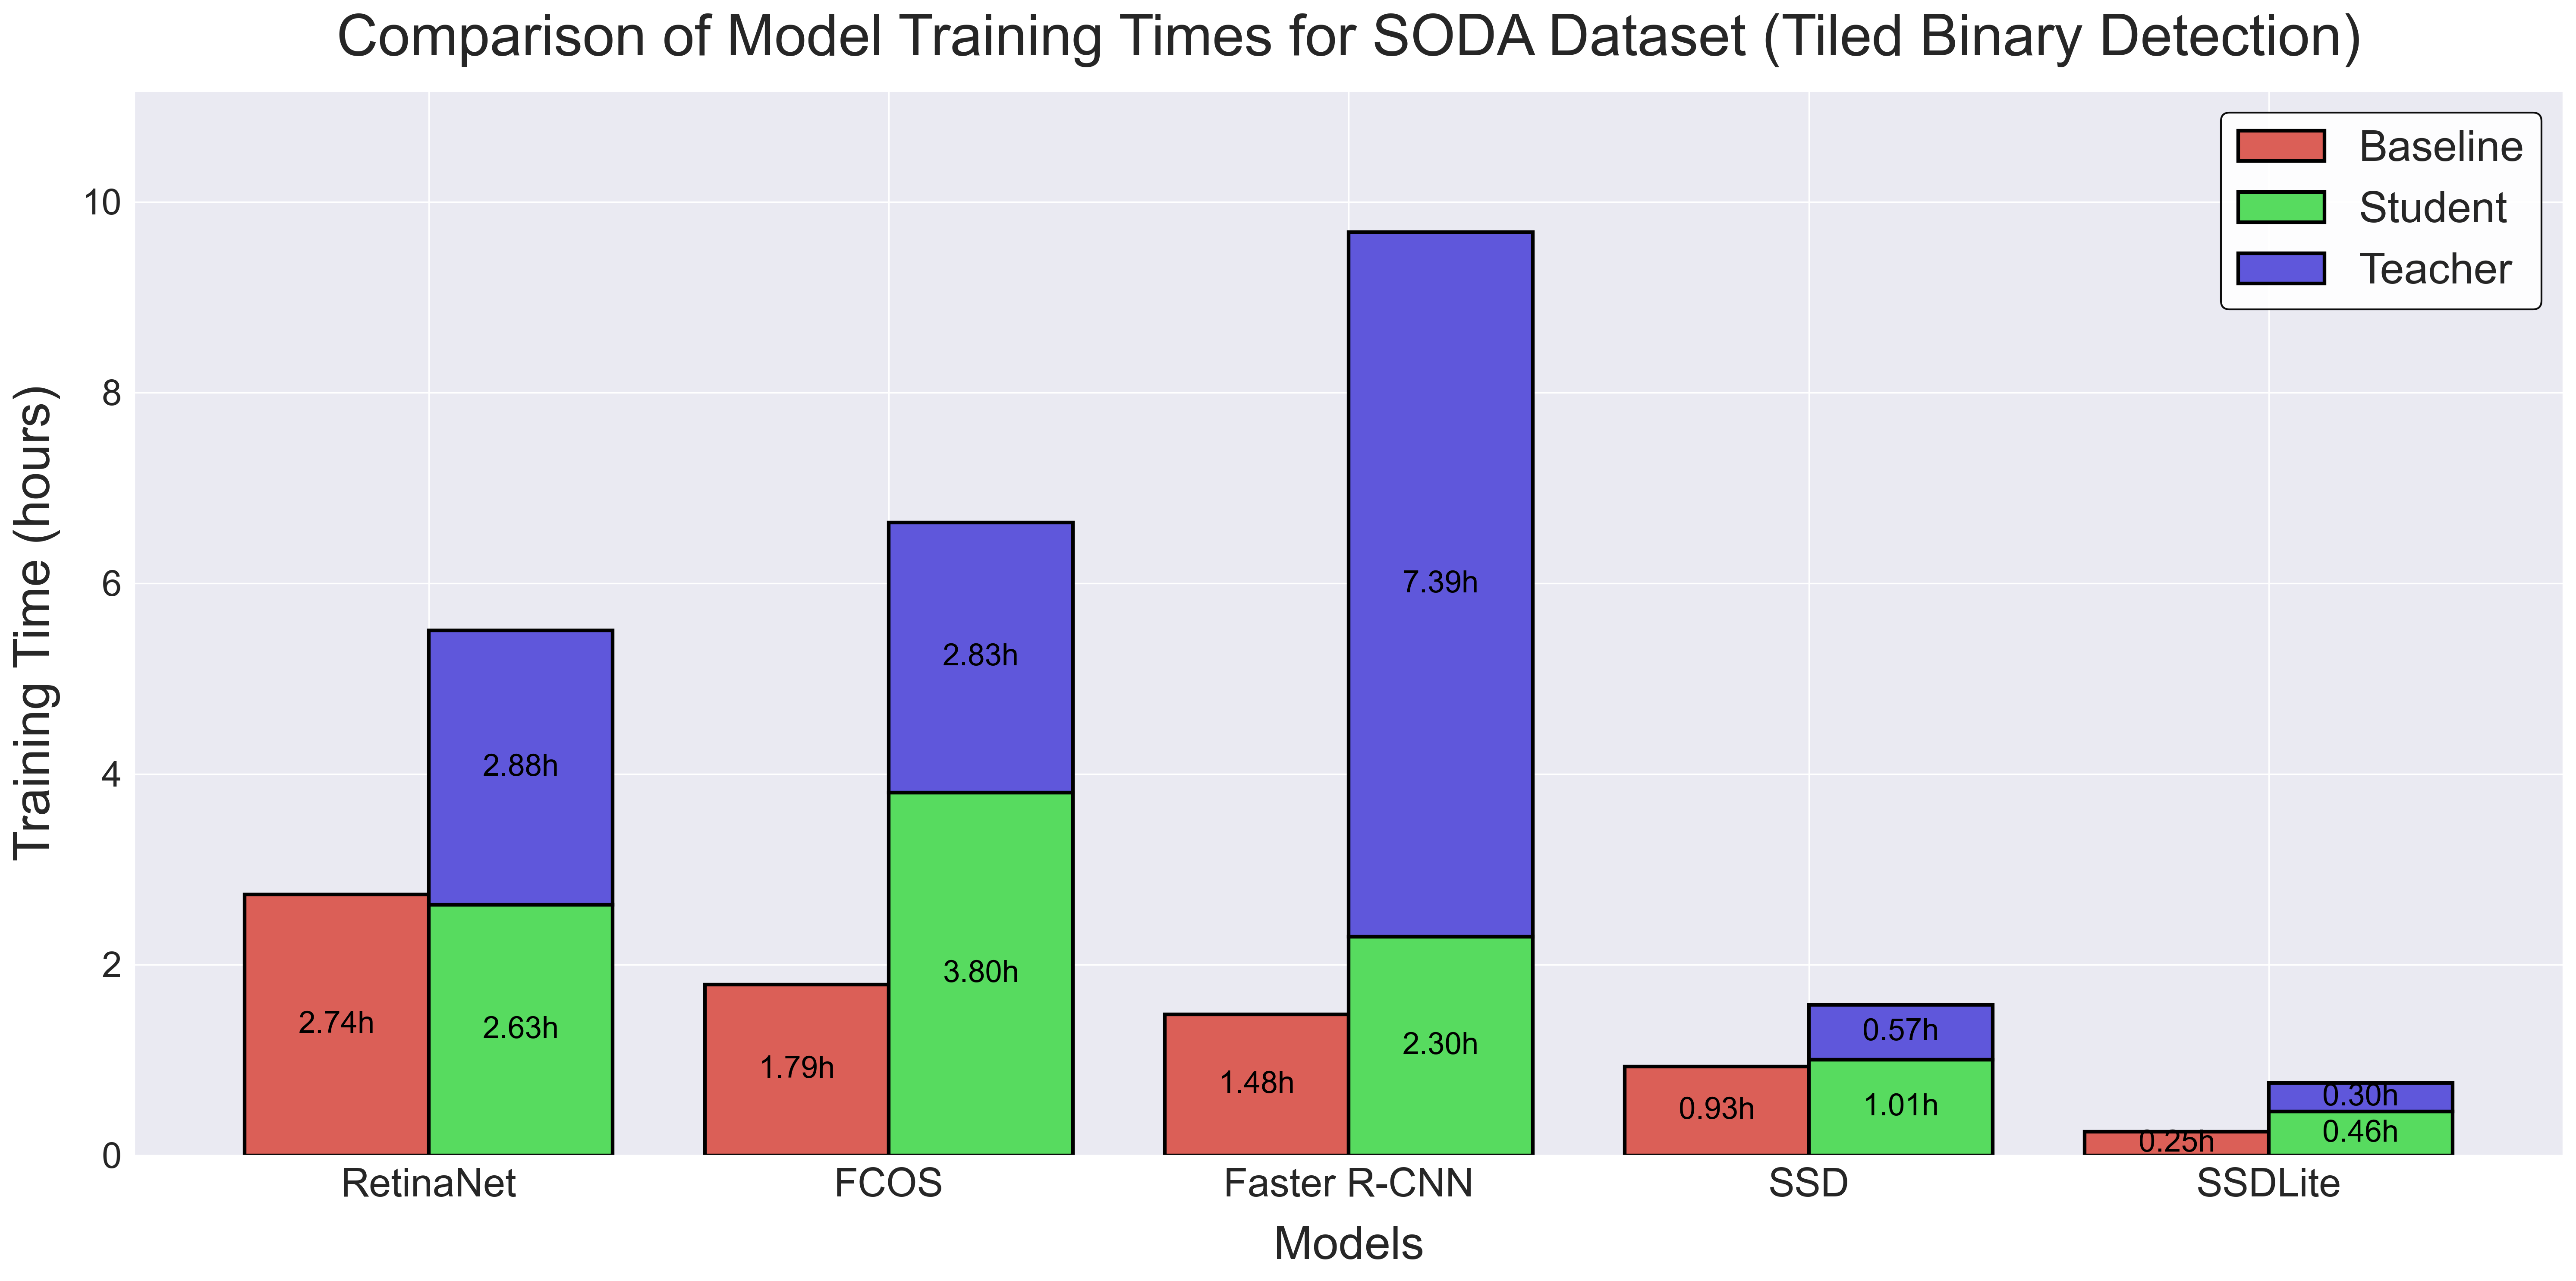
\includegraphics[width=1\textwidth]{training_times_soda_dataset_tiled_binary_detection.png}
    \caption{Comparison of model training times on the 3$\times$3 tiled \gls{soda} dataset across all altitudes for binary litter detection.}
    \label{fig:soda_tiled_single_training_time}
\end{figure}

Due to the increased number of training images, the overall time required rose across all models. For the \gls{ssd} and SSDLite models, both the student and baseline versions required roughly the same duration to complete training. Nevertheless, two further observations stand out. The \gls{fcos} student model took longer to train than its teacher, which might be explained by the added computational cost of the \textit{centre-ness} loss function. This component introduces further complexity to the optimisation process and could account for the increased training time. Additionally, the Faster \gls{rcnn} teacher exhibited a comparatively long training duration. However, the difference in training time between the Faster \gls{rcnn} student and its baseline counterpart was minimal.

Interestingly, the Faster \gls{rcnn} student model required less training time than the RetinaNet student, despite achieving the highest accuracy among all student models. This performance could be partly explained by the versatility of the region proposal mechanism used by the network.

A comparison of model sizes, as shown in Table~\ref{tab:model_configs_soda_tiled_single}, reveals results identical to those in Table~\ref{tab:model_configs_soda01m} from the first experiment. This consistency is due to the use of binary detection models, meaning the model heads remained the same. Despite this, the observed improvement in detection accuracy across most model architectures indicates that student models benefit from the inclusion of \gls{lupi}, without introducing any additional cost in terms of model size or computational load during inference.

\begin{table}[!ht]
    \centering
    \begin{tabular}{llcc}
        \toprule
        \textbf{Model Configuration} & \textbf{Type} & \textbf{Size (MB)} & \textbf{Parameters (M)} \\
        \midrule
        \multirow{5}{*}{\textbf{Baseline}} 
            & RetinaNet     & 122.72 & 32.17 \\
            & FCOS          & 122.32 & 32.06 \\
            & Faster R-CNN  & 157.54 & 41.30 \\
            & SSD           & 90.58  & 23.75 \\
            & SSDLite       & 8.42   & 2.21 \\
        \midrule
        \multirow{5}{*}{\textbf{Student}} 
            & RetinaNet     & 122.72 & 32.17 \\
            & FCOS          & 122.32 & 32.06 \\
            & Faster R-CNN  & 157.54 & 41.30 \\
            & SSD           & 90.58  & 23.75 \\
            & SSDLite       & 8.42   & 2.21 \\
        \bottomrule
    \end{tabular}
    \caption{Comparison of model configurations for trained baseline and student models on the 3$\times$3 tiled \gls{soda} dataset across all altitudes for binary litter detection, including model type, size in megabytes, and number of parameters (in millions).}
    \label{tab:model_configs_soda_tiled_single}
\end{table}

Overall, this experiment sought to introduce a more challenging setting in which to evaluate the proposed methodology by extending the scope of the 1-metre experiment to incorporate altitude as an additional practical factor. This added dimension increased the task's difficulty. Despite this, the use of \gls{lupi} continued to show improved accuracy in most models, although not universally. A noticeable decline was observed across all metrics, reflecting the increased complexity of the problem being addressed.


\subsection{Multi-label Litter Detection on the SODA Dataset Across All Altitudes}
\label{subsec:5_soda_tiled_multi_dataset_exp}
% Glorja lil Missier u lil Iben u lil Ispirtu s-Santu

The third experiment aimed to build upon the context established in the second, focusing again on multi-altitude \gls{uav}-based litter detection. However, this time, the objective was to test the method’s generalisability in a multi-label detection setting. The experimental setup remained consistent with the previous trials, though the model heads were reconfigured to classify six distinct litter categories, as defined in the 3$\times$3 tiled \gls{soda} dataset. This dataset comprised 7,461 images, of which 5,238 were used for training, 765 for validation, and 1,458 for testing.
This experiment posed a significantly greater challenge for the detection models. The task required accurate identification of small, visually similar litter types, often set against complex and varied backgrounds. The difficulty of distinguishing between these categories introduced a new layer of complexity.

The results, comparing the baseline models with the best-performing student models across the five selected detection architectures, are illustrated in Figure~\ref{fig:soda_tiled_multi_bar}. In most cases, the student models outperformed their baselines, with improvements particularly evident in the more demanding \gls{map}@50–95 metric. Additional gains were seen in precision, recall, and F1 scores. However, these improvements were notably smaller than those observed in the previous experiments. Given this added complexity, detection accuracy declined across all models, with low metric scores observed throughout. The \gls{ssd} and SSDLite architectures in particular showed little to no improvement under these conditions, further exacerbating their limitations in the context of \gls{uav}-based detection.

\begin{figure}[!ht]
    \centering
    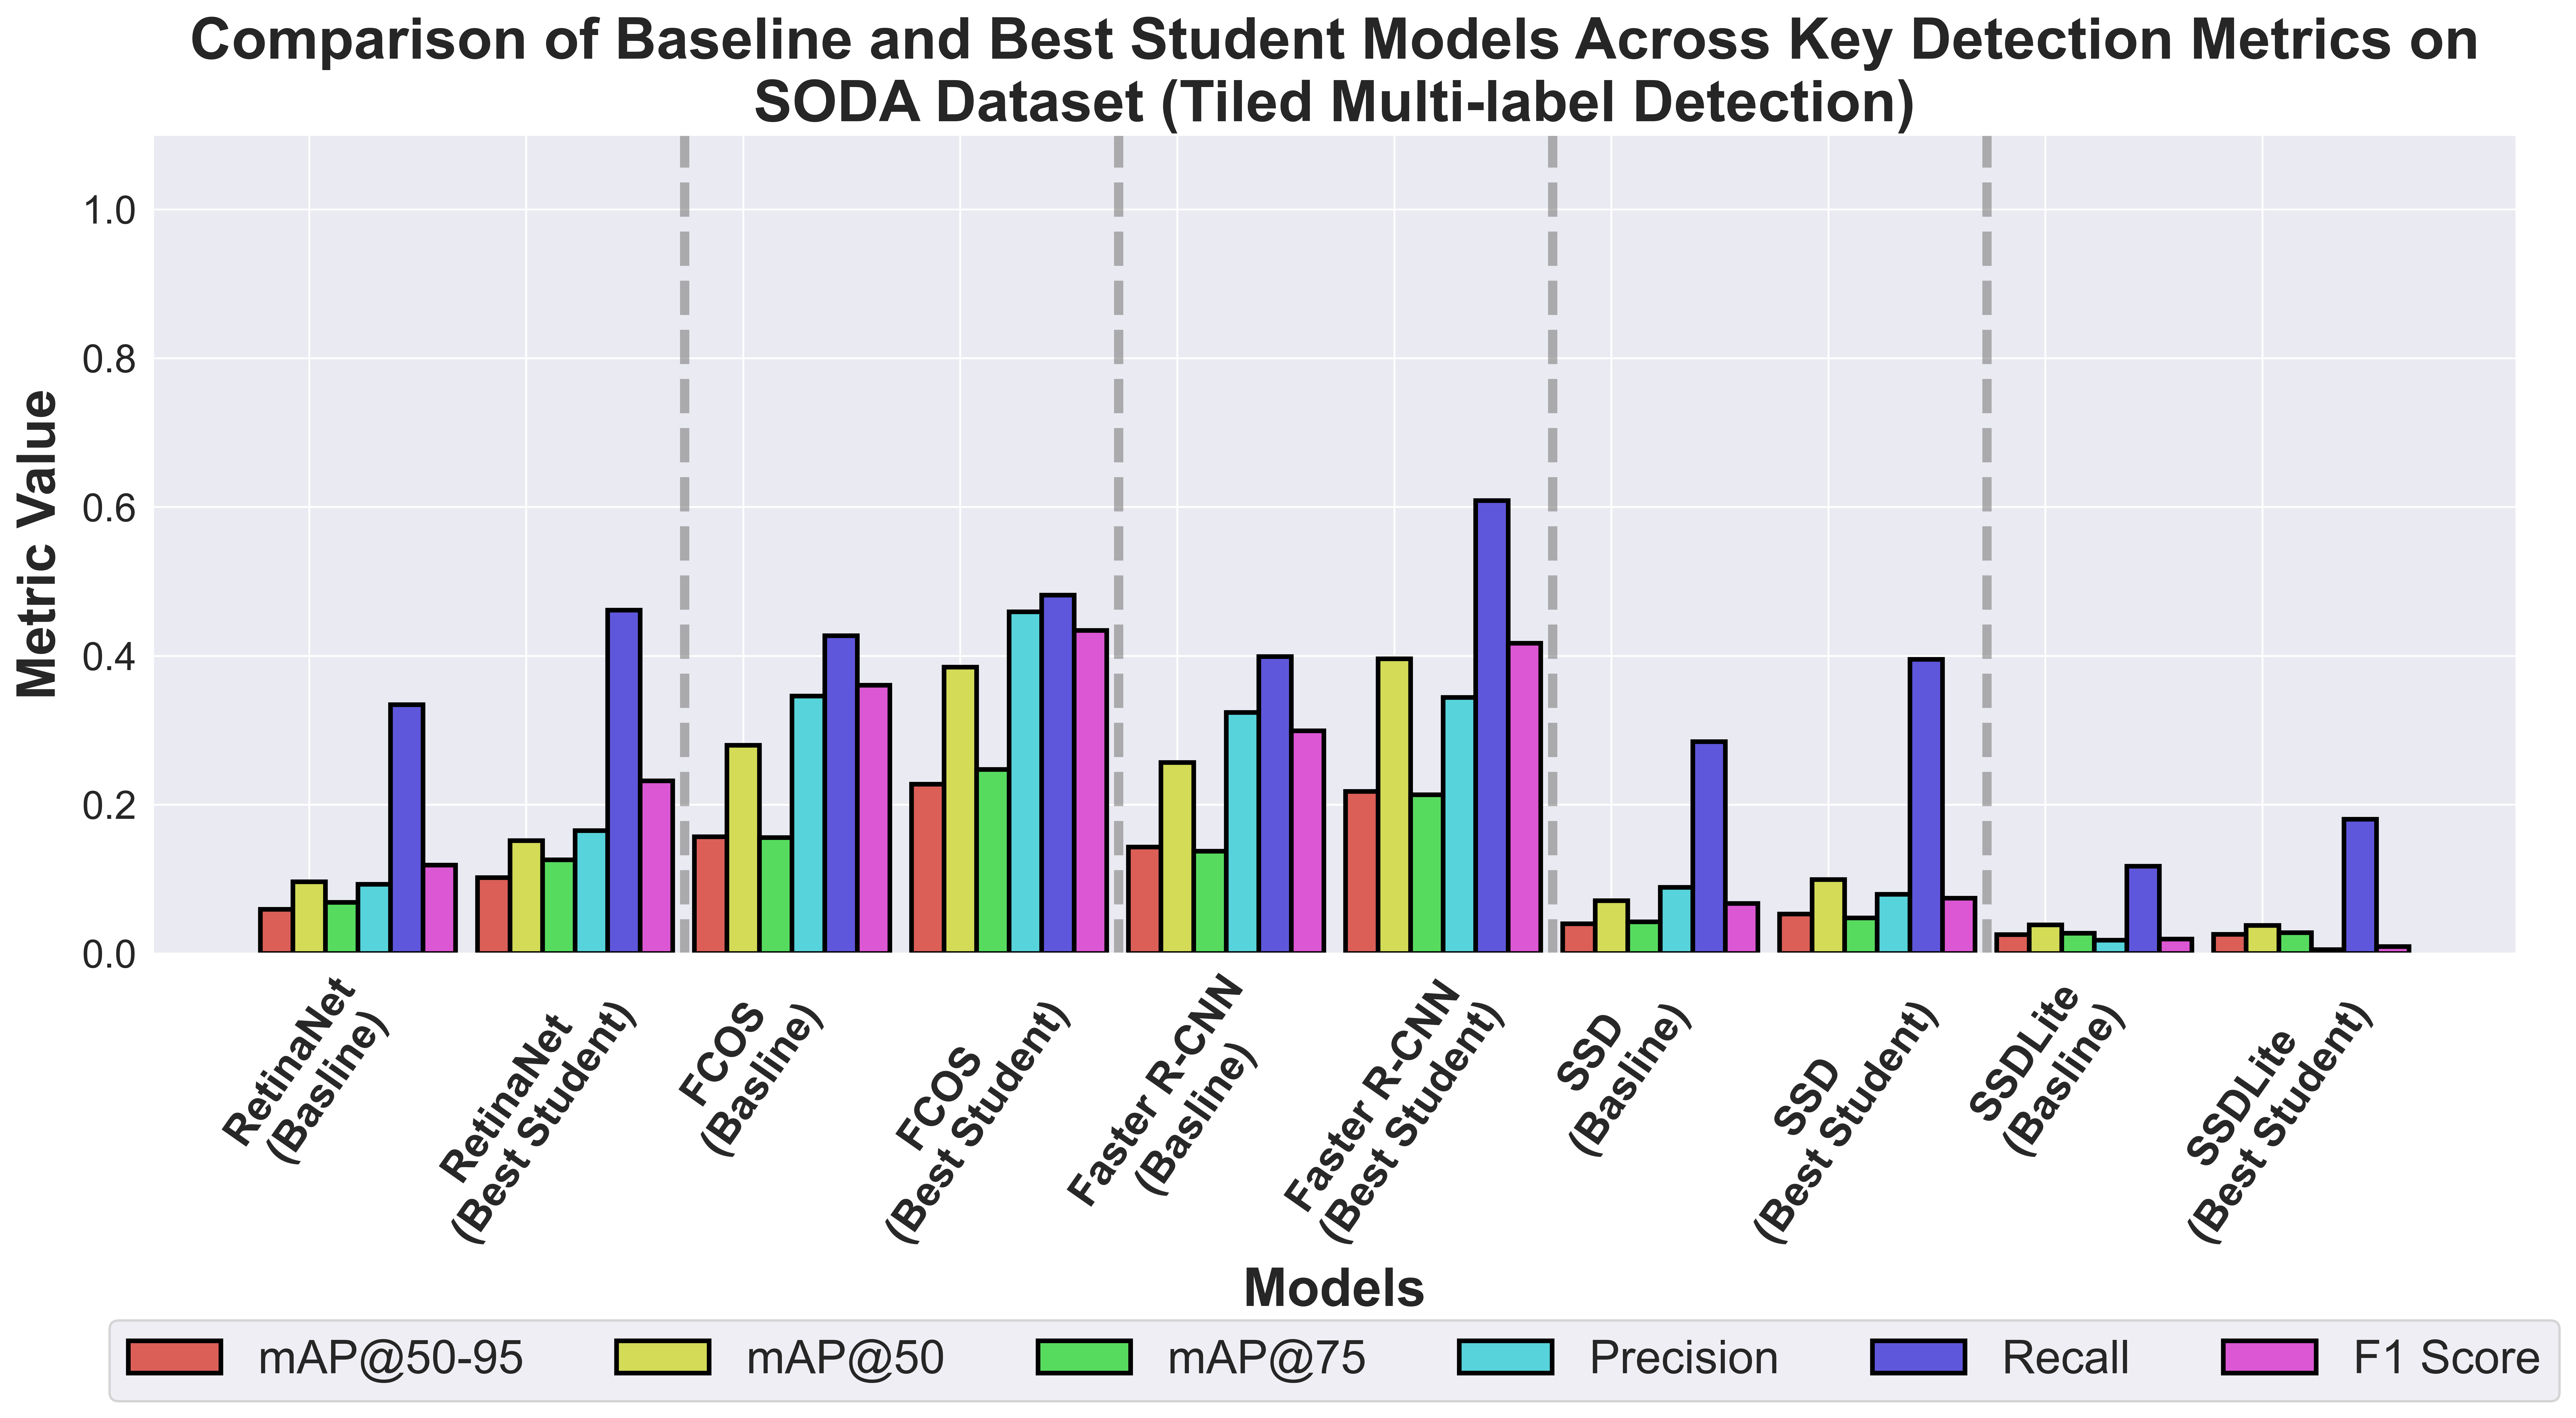
\includegraphics[width=1\textwidth]{SODA Dataset (Tiled Multi-label Detection).png}
    \caption{Comparison between the baseline and best-performing student models across key detection metrics on the 3$\times$3 tiled \gls{soda} dataset across all altitudes for multi-label litter detection.}
    \label{fig:soda_tiled_multi_bar}
\end{figure}

Compared to the earlier experiments, this setup presented a more difficult detection scenario, leading to an overall drop in performance. Nevertheless, models trained using the \gls{lupi} framework continued to show a measurable advantage in most cases.
Among all the models, the student version of \gls{fcos} delivered the best overall results, followed by Faster \gls{rcnn} and RetinaNet. While this represents a shift from previous experiments, the general trend suggests that architectures using the ResNet-\gls{fpn} backbone tend to be more effective for this litter detection task. For all-altitude binary litter detection, Faster \gls{rcnn} produced the best results, but in the multi-label detection experiment, \gls{fcos} was more effective. However, the differences between the two were minimal in both experiments.
Furthermore, the student models outperformed their baseline counterparts across all evaluated metrics, with accuracy improvements ranging from 0.01 to 0.08. Although these improvements gradually decreased, they still had a notable impact. \gls{fcos} and Faster \gls{rcnn} showed the most significant performance boosts compared to their baselines. RetinaNet and \gls{ssd} also showed some benefit, though to a lesser degree. In contrast, SSDLite showed no improvement in any of the metrics.

Having addressed multi-label detection, a class-specific analysis of detection accuracy was also conducted. Figure~\ref{fig:soda_tiled_multi_per_class} presents this evaluation using the \gls{ap}@50--95 metric. As seen, the same trend in model performance is maintained across architecture types. \gls{fcos} and Faster \gls{rcnn} again emerged as the best-performing models, followed by RetinaNet, \gls{ssd}, and SSDLite. The advantage offered by the \gls{lupi} framework is particularly evident here, with student models outperforming their baseline counterparts in most individual \gls{ap} scores.

\begin{figure}[!ht]
    \centering
    \includegraphics[width=1\textwidth]{map_all_classes_soda_multi.png}
    \caption{Comparison between the baseline and best-performing student models based on mean average precision by class on the 3$\times$3 tiled \gls{soda} dataset across all altitudes for multi-label litter detection.}
    \label{fig:soda_tiled_multi_per_class}
\end{figure}

When this performance is compared against the class imbalance found in the \gls{soda} dataset, as shown in Figure~\ref{fig:soda_annotation_distribution}, a consistent pattern is observed. The classes \textit{Drink Can} and \textit{Clear Plastic Bottle}, which are most frequent in the dataset, tend to record the highest \gls{ap} scores. Curiously, although \textit{Glass Bottle} is more common than several other classes, no detector in this study successfully identified it. This could be attributed to it being misclassified as \textit{Glass Jar}, due to the visual similarity between the two, leading to incorrect predictions.

Unexpectedly, \textit{Other Plastic Bottle} performed quite well despite its relatively low frequency in the dataset. This suggests that, in the context of litter detection across varied backgrounds, this particular class may present more distinct visual features, making it easier to detect than more transparent items, which blend more easily with their surroundings.

In addition to the class-specific results, the confusion matrix for this approach provides further insight, as shown in Figure~\ref{fig:cm_soda}. This figure presents the normalised confusion matrix for the best-performing model, \gls{fcos}. Both baseline and student versions exhibit a broadly diagonal structure, which is expected in successful classification scenarios. However, a considerable number of litter items remain unclassified, indicating a high rate of missed detections. Moreover, a portion of the litter is misclassified under incorrect categories, suggesting a degree of confusion between visually similar classes.

\begin{figure}[!ht]
  \centering
  \begin{tabular}{cc}
    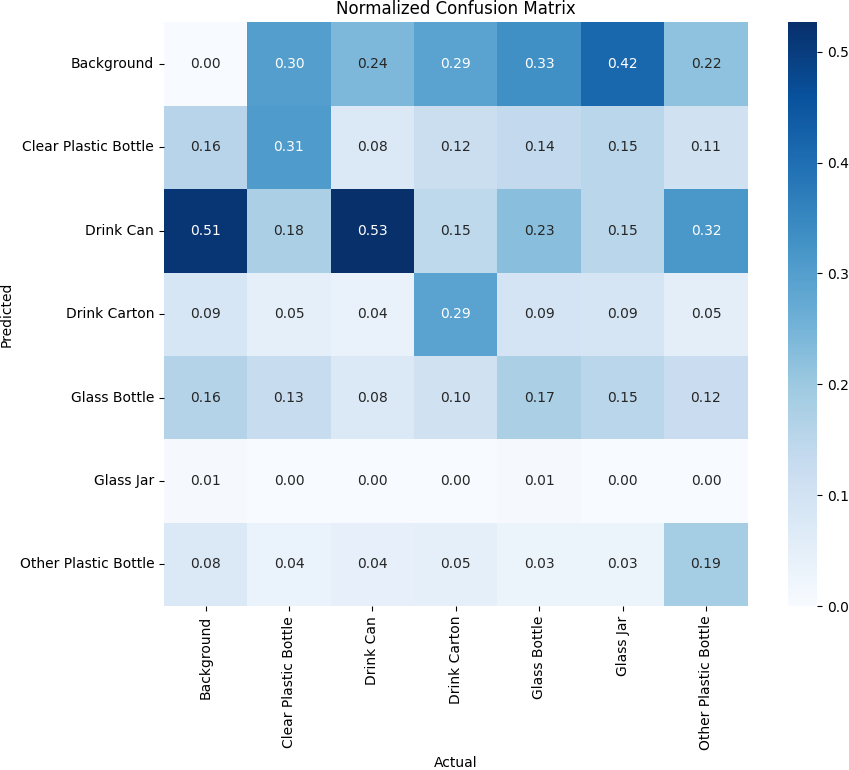
\includegraphics[width=0.48\textwidth]{cm1.png} &
    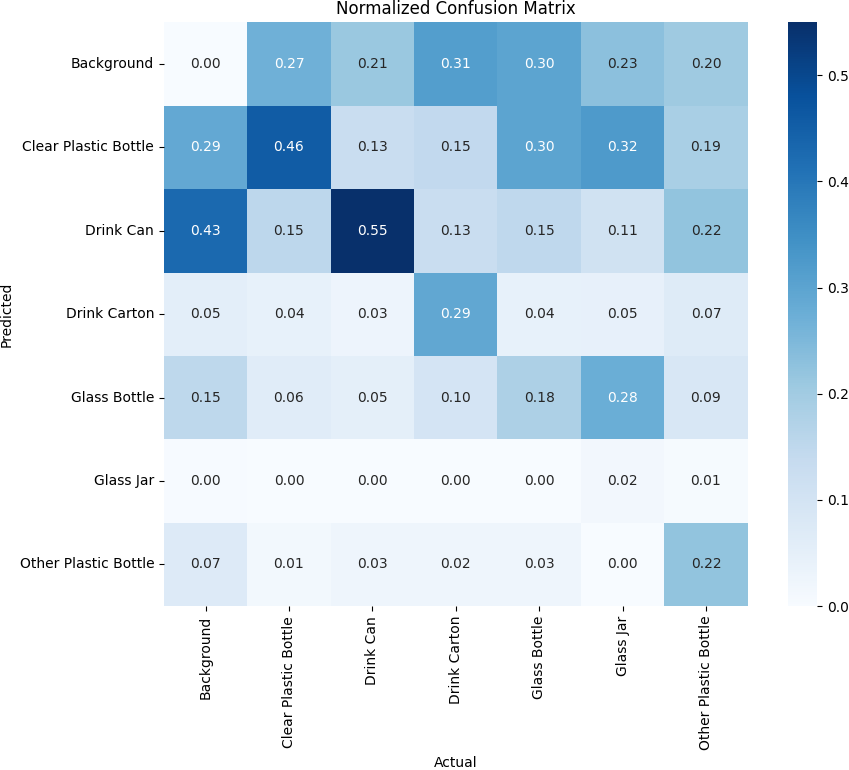
\includegraphics[width=0.48\textwidth]{cm2.png} \\
    \small (a) & \small (b) \\
  \end{tabular}
  \caption{Normalised confusion matrices for multi-label litter detection on the 3$\times$3 tiled \gls{soda} dataset across all altitudes, using the best-performing models of the \gls{fcos} architecture: (a) baseline model, (b) student model.}
  \label{fig:cm_soda}
\end{figure}

Notably, the student model demonstrates an improvement in this regard. The confusion matrix reveals stronger diagonal values across most categories, indicating better classification accuracy. Additionally, there are fewer unclassified instances, though a slight increase in misclassifications is also evident. These patterns support the overall finding that adopting the \gls{lupi} framework contributes positively to model performance.
Finally, the matrix highlights the underlying issue of class imbalance in the dataset. As previously outlined, categories with higher representation tend to achieve better scores.

In addition to the above comparisons, an extended analysis was conducted to evaluate the effectiveness of different teacher models, following a procedure consistent with the earlier experiments. The results, summarised in Table~\ref{tab:teacher_model_metrics_soda_tiled_multi}, report the detection accuracy achieved by each teacher architecture. As previously observed, Faster \gls{rcnn}, \gls{fcos}, and RetinaNet remained the strongest performers, with many of their metrics approaching values that suggest effective learning of the target concept. While minor declines were observed across several metrics, the increase in the \gls{mar}@1 score may reflect improved top-ranked predictions, though it does not necessarily indicate a broader improvement in recall performance. These findings imply that, even with the added complexity of the scenes, these models continue to perform reliably in terms of detection accuracy.

\begin{table}[!ht]
    \centering
    \begin{adjustbox}{max width=\textwidth}
    \renewcommand{\arraystretch}{1.5}
    \begin{tabular}{|l|c|c|c|c|c|c|c|c|c|}
        \hline
        \textbf{Model} & \textbf{mAP@50--95} & \textbf{mAP@50} & \textbf{mAP@75} & \textbf{mAR@1} & \textbf{mAR@10} & \textbf{mAR@100} & \textbf{Precision} & \textbf{Recall} & \textbf{F1 Score} \\ \hline \hline
        \textbf{RetinaNet} & 0.88 & 0.92 & 0.91 & 0.66 & 0.89 & 0.89 & 0.76 & 0.97 & 0.85 \\\hline
        \textbf{FCOS} & 0.91 & 0.95 & 0.94 & 0.68 & 0.92 & 0.92 & 0.91 & 0.97 & 0.94 \\\hline
        \textbf{Faster R-CNN} & \textbf{0.95} & \textbf{0.99} & \textbf{0.98} & \textbf{0.70} & \textbf{0.96} & \textbf{0.96} & \textbf{0.96} & \textbf{0.99} & \textbf{0.97} \\\hline
        \textbf{SSD} & 0.36 & 0.49 & 0.45 & 0.33 & 0.41 & 0.41 & 0.59 & 0.76 & 0.63 \\\hline
        \textbf{SSDLite} & 0.11 & 0.13 & 0.13 & 0.13 & 0.13 & 0.13 & 0.00 & 0.37 & 0.01 \\
        \hline
    \end{tabular}
    \renewcommand{\arraystretch}{1}
    \end{adjustbox}
    \caption{Comparison of teacher model performance across key detection metrics, trained on the 3$\times$3 tiled \gls{soda} dataset across all altitudes for multi-label litter detection.}
    \label{tab:teacher_model_metrics_soda_tiled_multi}
\end{table}
 
The \gls{ssd} and SSDLite teacher models once again displayed a marked drop in detection accuracy, both in comparison to other architectures and relative to their own performance in the preceding experiment. This further exacerbates their limited capacity to generalise within this more demanding detection context. As observed previously, Faster \gls{rcnn} remained the most effective teacher model overall. However, despite being the second-best teacher, \gls{fcos} produced the highest-performing student in this multi-label setup. RetinaNet continued to lag behind both Faster \gls{rcnn} and \gls{fcos}, showing comparatively weaker performance.
Among all teacher models, recall scores were consistently high, while precision varied more significantly. Notably, SSDLite recorded a precision score of zero, whereas the remaining models achieved more acceptable precision values, ranging from 0.59 to 0.96.

The training durations for all models used in this experiment are shown in Figure~\ref{fig:soda_tiled_multi_training_time}. These results contrast significantly with those from the first experiment (see Figure~\ref{fig:soda_tiled_single_training_time}). Overall, training times increased across the board. Notably, the student models required substantially more time to train compared to their baseline counterparts, marking a sharp rise relative to the earlier experiment.

\begin{figure}[!ht]
    \centering
    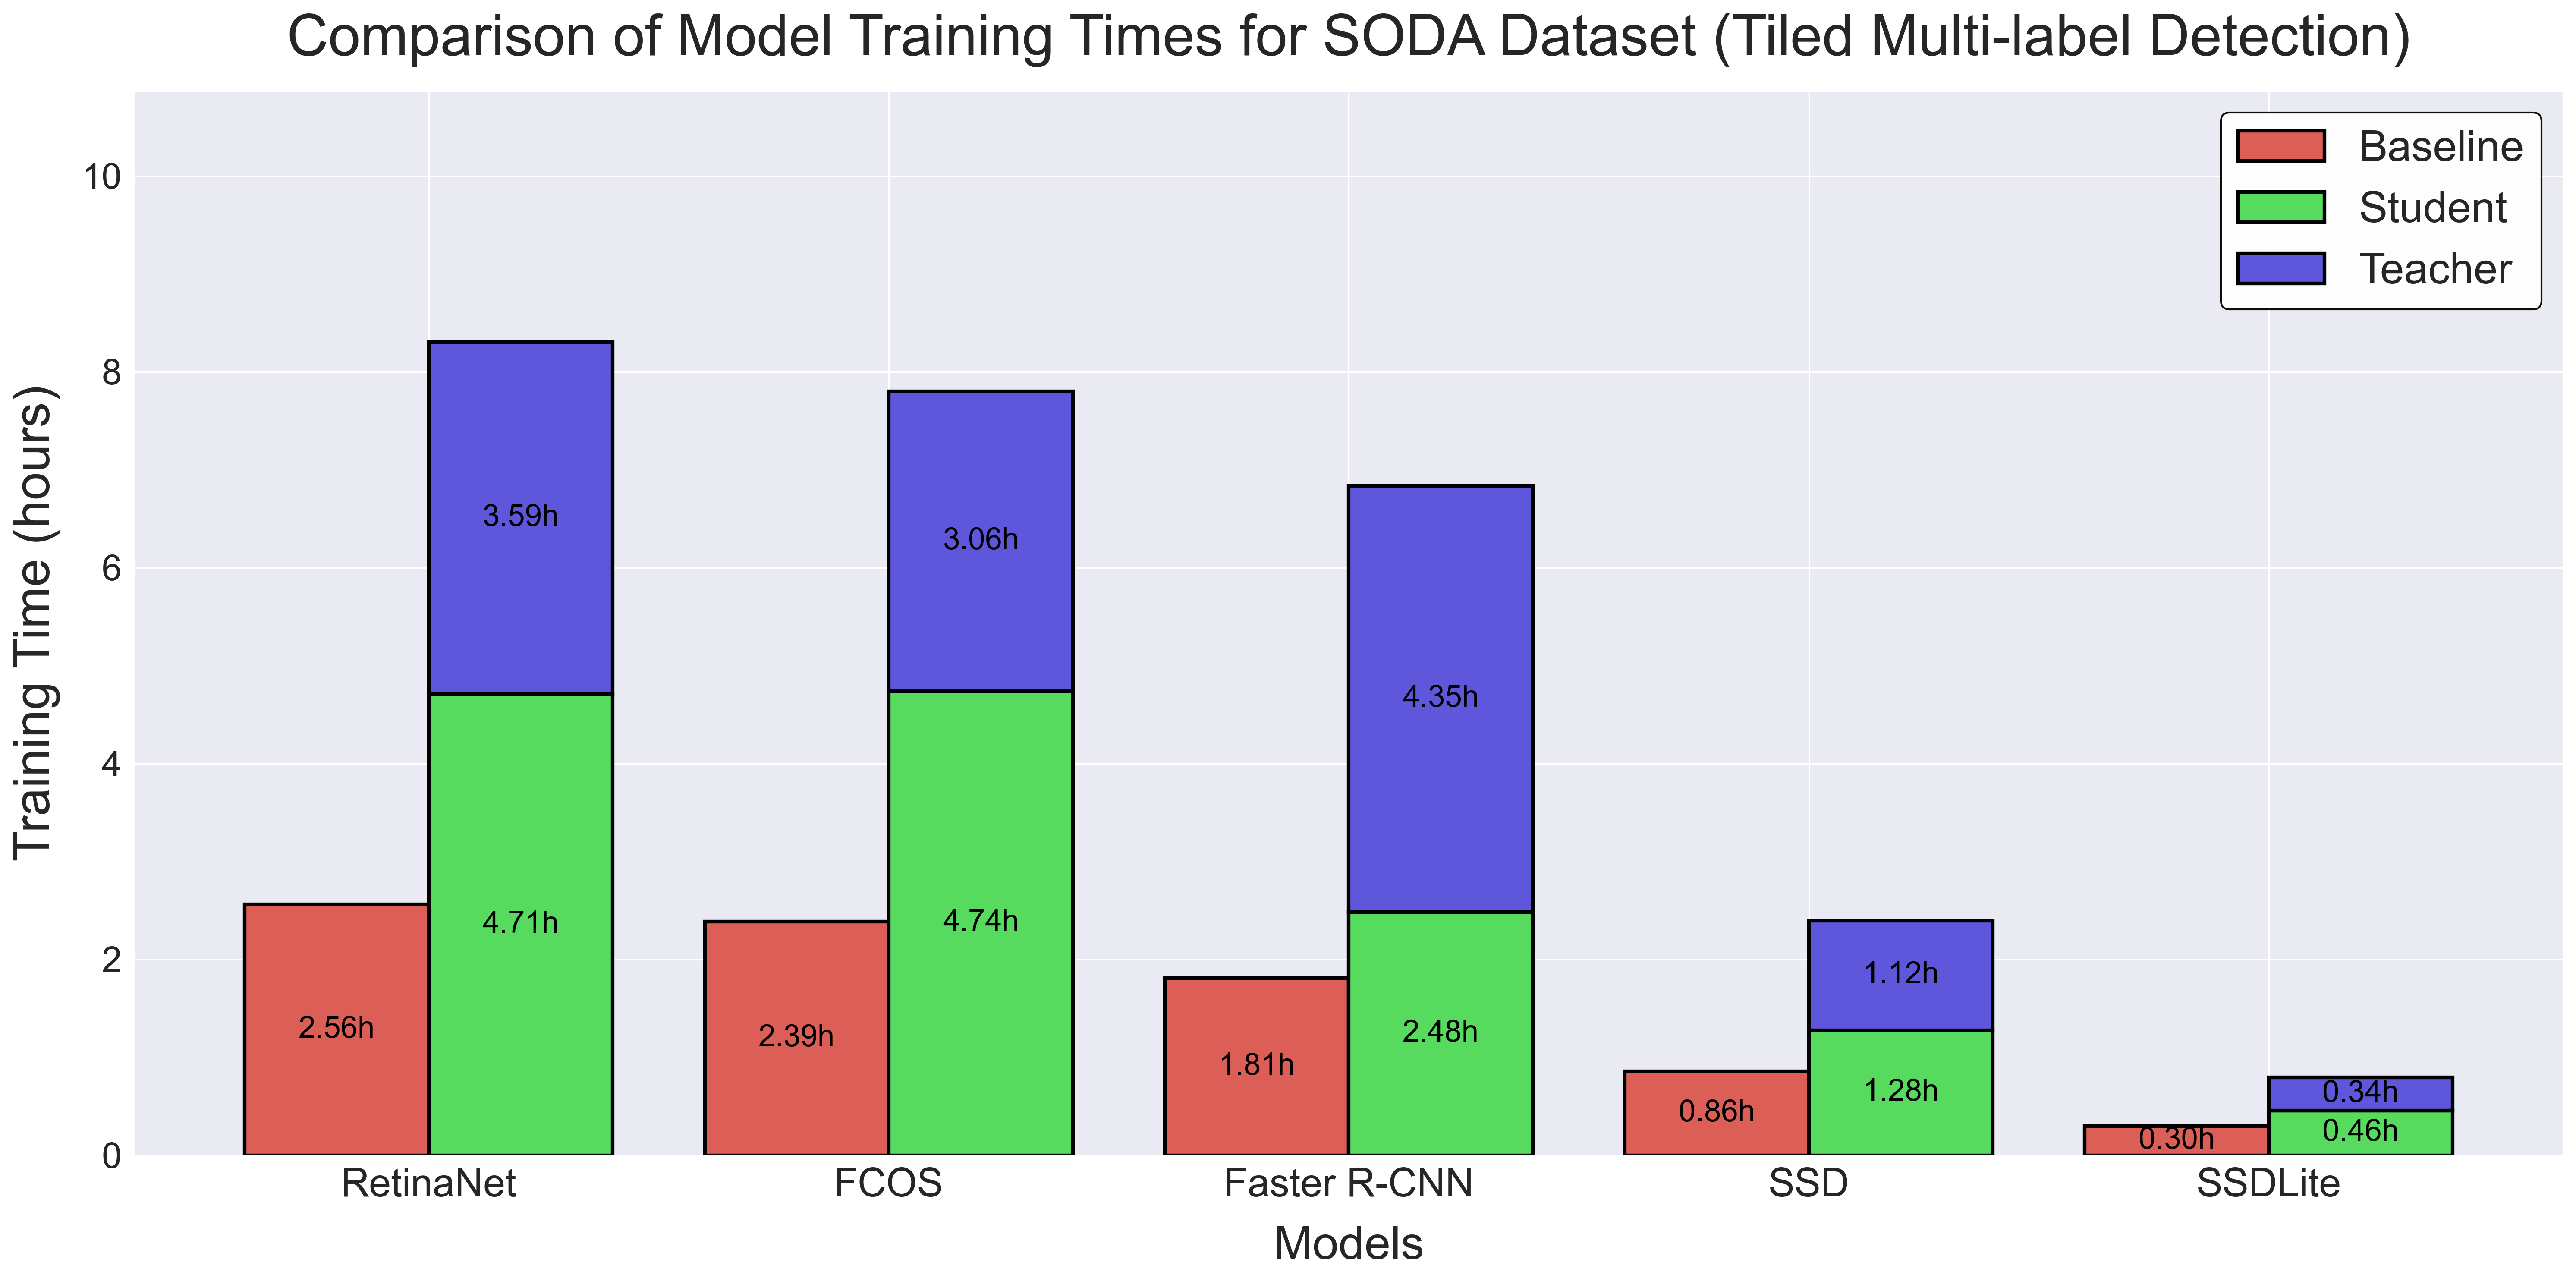
\includegraphics[width=1\textwidth]{training_times_soda_dataset_tiled_multi_label_detection.png}
    \caption{Comparison of model training times on 3$\times$3 tiled \gls{soda} dataset across all altitudes for multi-label litter detection.}
    \label{fig:soda_tiled_multi_training_time}
\end{figure}

Interestingly, the teacher models now required less training time than their corresponding student models, a trend observed across all architectures except for Faster \gls{rcnn}. The \gls{fcos} student model, despite requiring more training time than RetinaNet, achieved the best performance overall. In contrast, Faster \gls{rcnn} trained faster than RetinaNet, and both Faster \gls{rcnn} and \gls{fcos} required less cumulative time for training (teacher and student combined) than the RetinaNet model. Meanwhile, \gls{ssd} and SSDLite remained the fastest to train, maintaining a similar trend to that observed in previous experimental setups.

A comparison of model sizes, as outlined in Table~\ref{tab:model_configs_soda_tiled_multi}, reveals results that differ slightly from those observed in the previous experiments. This variation stems from the shift to multi-label detection, which required modifying the model head to predict a broader range of categories. Consequently, this adjustment led to an expected increase in the parameter count within the detection head, consistent with standard object detection practices. Nonetheless, the overall trend of improved detection accuracy across most model architectures suggests that student models continue to benefit from the application of \gls{lupi}, without incurring any added cost in terms of model size or computational demand during inference.

\begin{table}[!ht]
    \centering
    \begin{tabular}{llcc}
        \toprule
        \textbf{Model Configuration} & \textbf{Type} & \textbf{Size (MB)} & \textbf{Parameters (M)} \\
        \midrule
        \multirow{5}{*}{\textbf{Baseline}} 
            & RetinaNet     & 123.11 & 32.27 \\
            & FCOS          & 122.36 & 32.08 \\
            & Faster R-CNN  & 157.64 & 41.32 \\
            & SSD           & 93.13  & 24.41 \\
            & SSDLite       & 8.68   & 2.28 \\
        \midrule
        \multirow{5}{*}{\textbf{Student}} 
            & RetinaNet     & 123.11 & 32.27 \\
            & FCOS          & 122.36 & 32.08 \\
            & Faster R-CNN  & 157.64 & 41.32 \\
            & SSD           & 93.13  & 24.41 \\
            & SSDLite       & 8.68   & 2.28 \\
        \bottomrule
    \end{tabular}
    \caption{Comparison of model configurations for trained baseline and student models on the 3$\times$3 tiled \gls{soda} dataset across all altitudes for multi-label litter detection, including model type, size in megabytes, and number of parameters (in millions).}
    \label{tab:model_configs_soda_tiled_multi}
\end{table}

Across these experiments, which span various realistic contexts and model architectures, it has been demonstrated that incorporating \gls{lupi} in object detection results in improved performance in the majority of cases. In instances where little to no improvement was observed, this can generally be attributed to the limitations of the architecture itself, which may not be optimised to handle the specific detection task. Additionally, while there is a trade-off in terms of increased training time due to the necessity of training both a teacher and a student model, the overall model parameters and sizes remain unchanged with the adoption of this approach.

\section{Cross-Dataset Evaluation}
\label{sec:5_cross_dataset_exp}

In addition to the within-dataset evaluation, a separate cross-dataset examination was conducted to verify whether the models trained on the \gls{soda} dataset exhibited more consistent learning when trained with \gls{lupi}, compared to their baseline counterparts, in alignment with objective \textbf{O3}. To this end, cross-dataset testing was carried out using the two other available \gls{uav}-based litter detection datasets: \gls{bdw} and UAVVaste. For the \gls{bdw} dataset, models trained on the \gls{soda} dataset at 1-metre altitude were selected, given their closer alignment with the characteristics of the \gls{bdw} data (see Figure~\ref{fig:bdw_samples}). For the UAVVaste evaluation, the binary litter detection models trained on the 3$\times$3 tiled version of the \gls{soda} dataset were used, again due to the similarity in visual layout and scene composition (refer to Figure~\ref{fig:uavvaste_samples}). In both cases, the models applied were trained specifically for binary litter detection.

\subsection{Binary Litter Detection on the BDW Dataset}
\label{subsec:5_bdw_exp}

The results on the \gls{bdw} dataset, as shown in Figure~\ref{fig:bdw_bar}, demonstrate that student models trained using the proposed \gls{lupi}-based approach consistently outperformed their baseline counterparts across all architectures. For each detection metric, student models showed measurable improvements. In the more stringent \gls{map}@50--95, performance increased by between 0.04 and 0.13, while even larger margins were observed in metrics such as \gls{map}@50. Interestingly, although RetinaNet had been the top performer in the within-dataset evaluation for the 1-metre altitude experiment, it was \gls{fcos} that achieved the best results on the \gls{bdw} test subset, closely followed by RetinaNet and Faster \gls{rcnn}. \gls{ssd} also returned relatively high results, whereas SSDLite continued to trail behind the others.

\begin{figure}[!ht]
    \centering
    \includegraphics[width=1\textwidth]{BDW Dataset (Tested on Models Trained on SODA 01m Binary Detection).png}
    \caption{Comparison of baseline and best-performing student models on key detection metrics using the \gls{bdw} dataset. The evaluated models were trained on the \gls{soda} dataset captured at 1-metre altitude for binary litter detection.}
    \label{fig:bdw_bar}
\end{figure}

Models using the ResNet-\gls{fpn} backbone continued to perform reliably well, suggesting that this architecture suits the challenges of \gls{uav}-based litter detection. Overall, the results point to the value of integrating \gls{lupi}, which seems to produce models that adapt better and generalise more effectively across datasets. While training time is slightly worse, these benefits come without adding to the model’s size, which retains the method's efficiency and ease of deployment.


\subsection{Binary Litter Detection on the UAVVaste Dataset}
\label{subsec:5_uavvaste_exp}

The cross-dataset evaluation results on the UAVVaste dataset, shown in Figure \ref{fig:uavvaste_bar}, largely confirm the earlier trend: the proposed approach incorporating \gls{lupi} tends to improve detection performance for student models over their baseline counterparts. In this setup, the binary detection models trained on the 3$\times$3 tiled \gls{soda} dataset were evaluated on the UAVVaste data.

\begin{figure}[!ht]
    \centering
    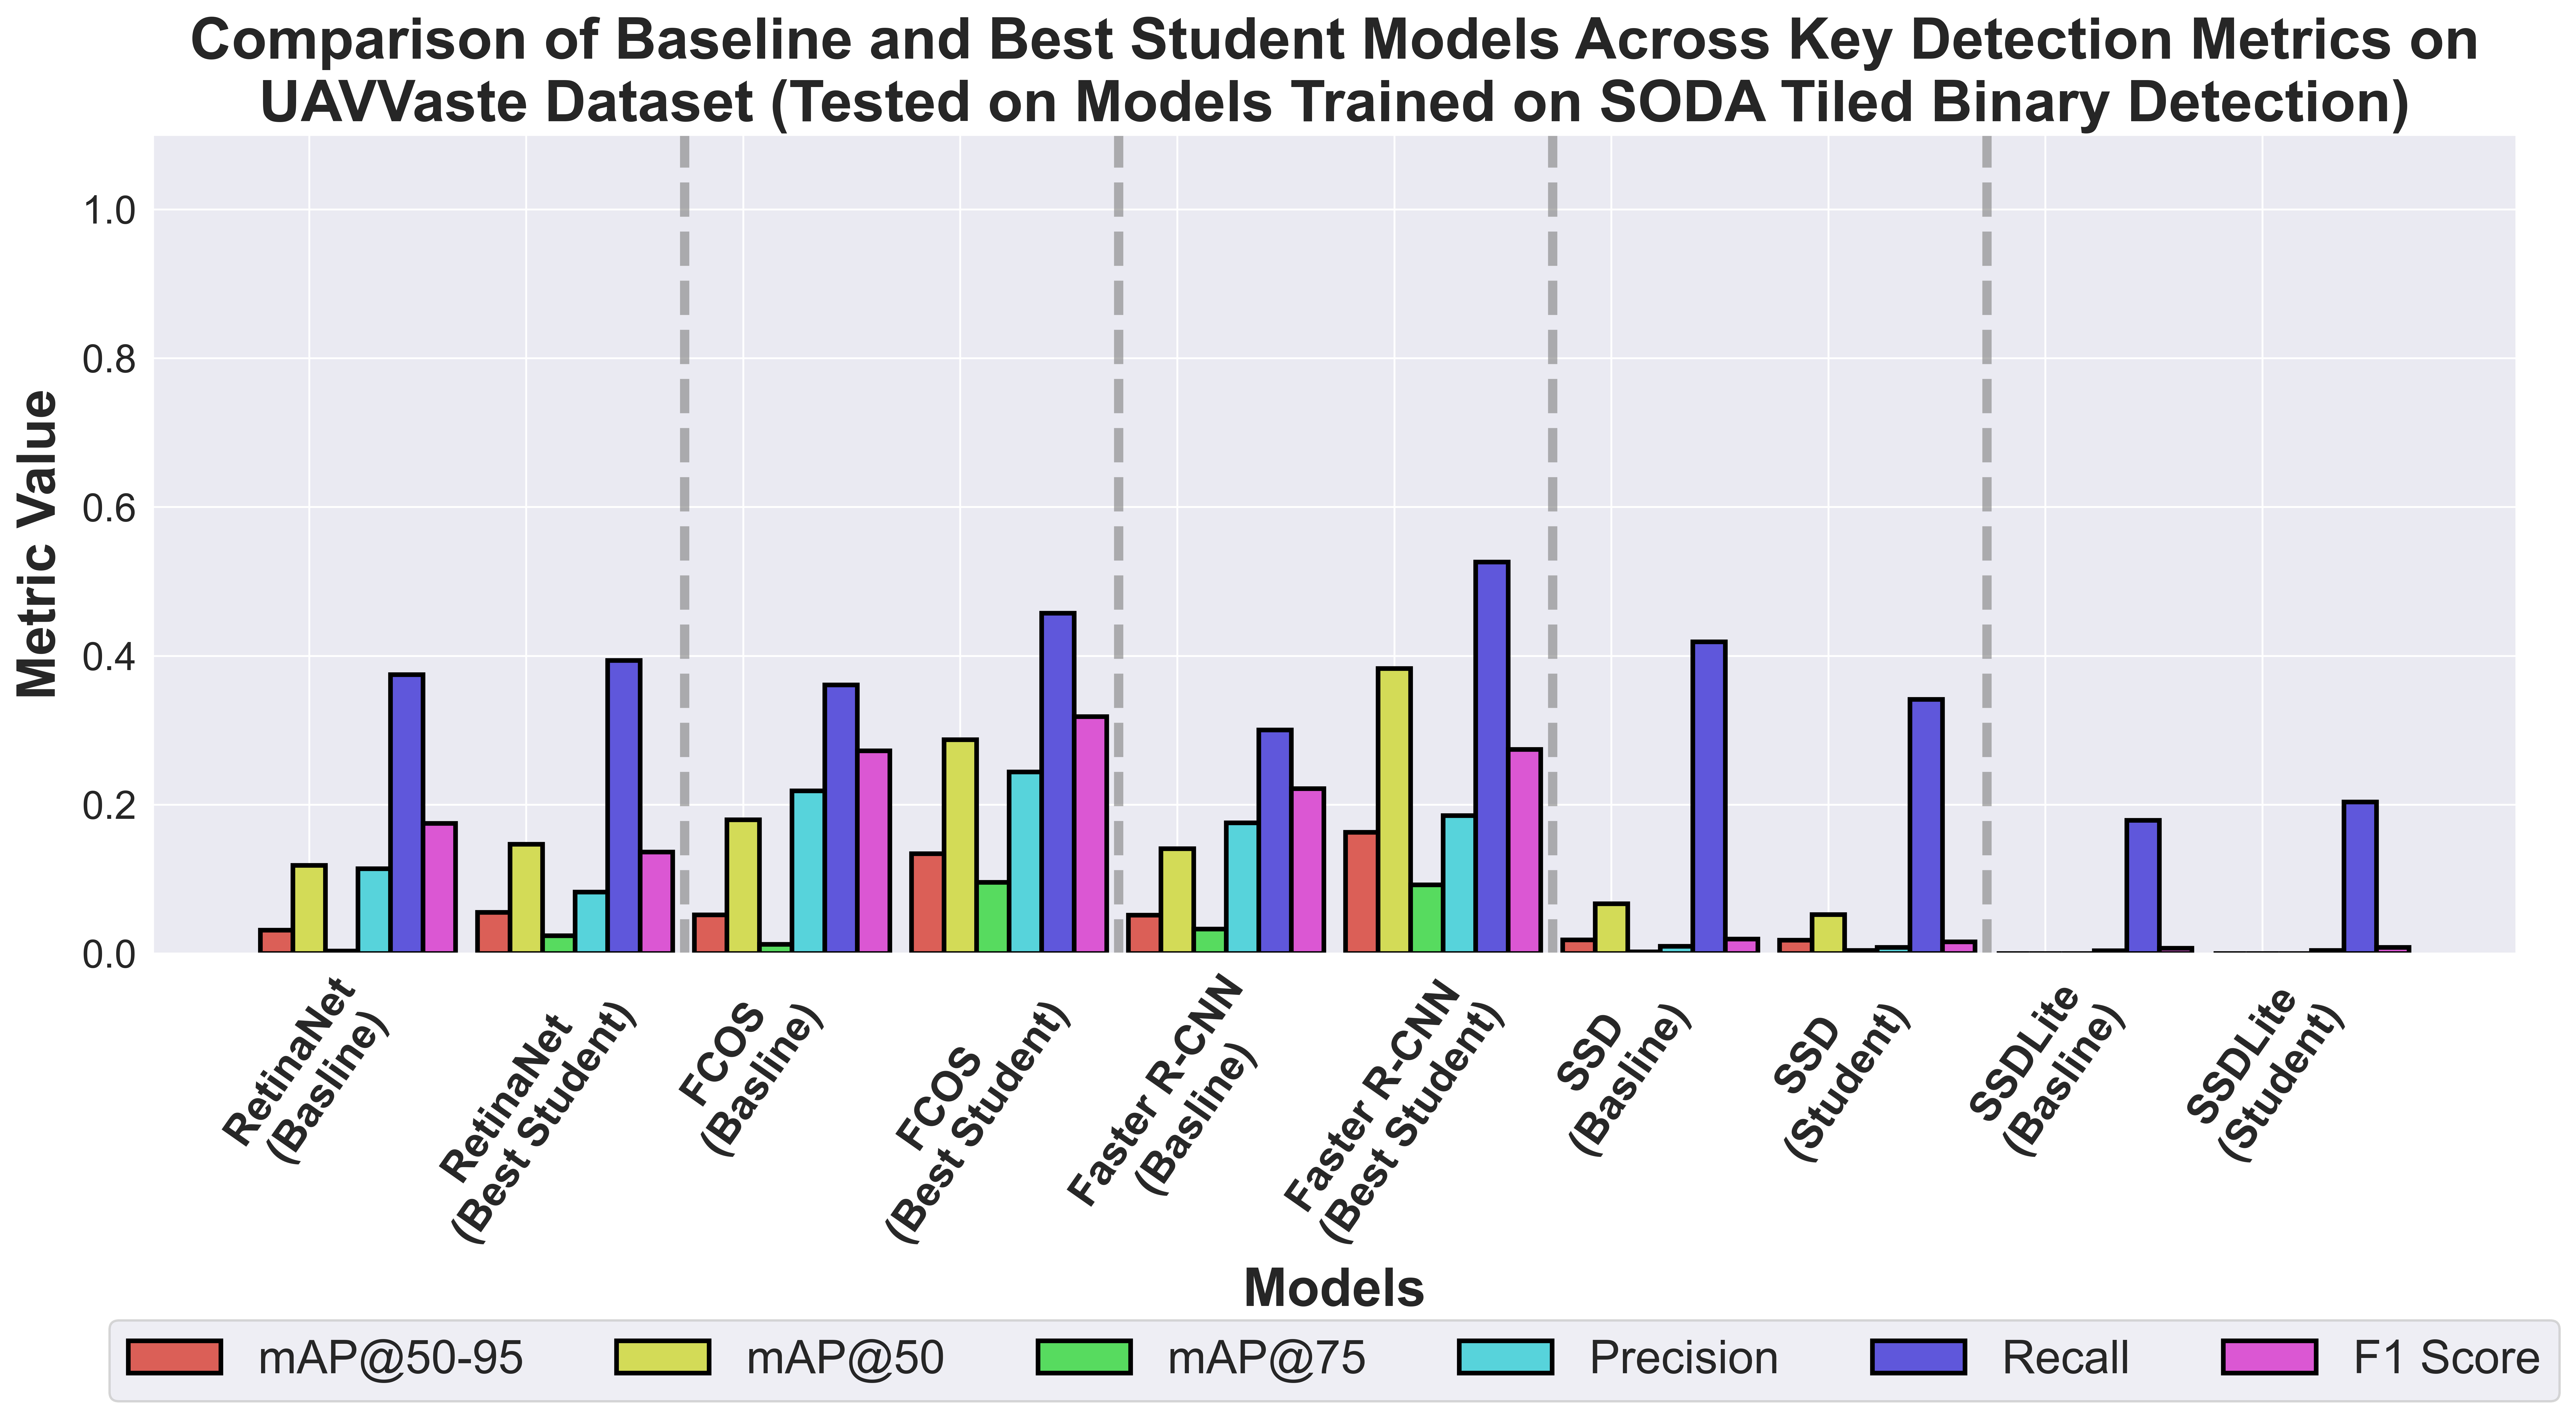
\includegraphics[width=1\textwidth]{UAVVaste Dataset (Tested on Models Trained on SODA Tiled Binary Detection).png}
    \caption{Comparison of baseline and best-performing student models on key detection metrics using the UAVVaste dataset. The evaluated models were trained on the 3$\times$3 tiled \gls{soda} dataset across all altitudes for binary litter detection.}
    \label{fig:uavvaste_bar}
\end{figure}

Faster \gls{rcnn}, \gls{fcos}, and RetinaNet all produced stronger results under the student setting, showing an improvement of around 0.03 to 0.11 in the more demanding \gls{map}@50--95 metric. In contrast, SSDLite failed to register any successful detections, and \gls{ssd} yielded identical \gls{map}@50--95 scores between the student and baseline models, though with slightly lower performance in the other metrics for the student variant.

The weaker outcomes from SSDLite and \gls{ssd} once again highlight their unsuitability for \gls{uav}-based litter detection, suggesting that the limited improvements observed with \gls{lupi} stem from the inherent inefficiency of these architectures in addressing this task.
The drop in performance across all detectors likely stems from how litter is represented in each dataset. As shown in Figure \ref{fig:uavvaste_samples}, the UAVVaste dataset contains smaller and visually distinct litter representations compared to the \gls{soda} dataset. Even so, several models produced accurate predictions, with most student models outperforming their baseline counterparts.

\section{Pascal VOC 2012 Evaluation}
\label{sec:5_pascal_voc_dataset_exp}
% Sliema Ghalik Marija, bil Grazzja Mimlija, Imbierek il Frott tal Guf Tieghek Gesu', Qaddisa Marija Omm Alla Itlob ghalin il Midinbin, Issa u Fis Siegha tal mewt taghna. Amen. Grazzi

Although it has consistently been shown across both within-dataset and cross-dataset evaluations that integrating \gls{lupi} into object detection allows student models to outperform their baselines, proven even in demanding scenarios such as that of \gls{uav}-based litter detection and small object detection. A final experiment was conducted to verify the generalisability of the proposed approach across larger object detection datasets with a larger number of categories, addressing fully objective \textbf{O4}. To this end, the Pascal \gls{voc} 2012 dataset was selected for its broader range of object categories and increased complexity. With 20 object classes, the dataset provides a more challenging test environment. As detailed in Subsection \ref{subsec:4_pascal_voc}, Pascal VOC is a widely recognised benchmark for object detection. It contains 17,112 images in total, with 13,690 used for training and 3,422 for validation in this study.

The results of this experiment, comparing the baseline model with the best student model across five selected detection architectures, are shown in Figure \ref{fig:pascal_voc_bar}. In most architectures, the student model outperformed the baseline, demonstrating a marginal improvement in detection accuracy when compared to previous experiments, especially in the challenging \gls{map}@50–95 metric. Among the models tested, the SSDLite student achieved the highest performance, followed by Faster \gls{rcnn}, \gls{fcos}, and \gls{ssd} student models. Across all metrics, the student models showed an accuracy improvement ranging from 0.02 to 0.05, although slightly less when compared to the other models presented in this study.

\begin{figure}[!htbp]
    \centering
    \includegraphics[width=1\textwidth]{Pascal VOC 2012 Dataset (Multi-label Detection for 20 Classes) .png}
    \caption{Comparison between the baseline and best-performing student models across key detection metrics on the Pascal VOC 2012 dataset for multi-label detection of 20 object classes.}
    \label{fig:pascal_voc_bar}
\end{figure}

Unfortunately, the Faster \gls{rcnn} student architecture performed worse than its baseline counterpart, while \gls{ssd} and SSDLite models showed the largest improvements. Interestingly, the architectures using the ResNet-\gls{fpn} architecture performed relatively worse than the others, in contrast to the litter detection experiments. This can be attributed to the nature of the data, as Pascal \gls{voc} contains images at relatively smaller resolutions. This, combined with the initialisation of pre-trained weights from models trained on the \gls{coco} dataset (which contains images of higher resolution), may have contributed to this performance discrepancy. On the other hand, \gls{ssd} and SSDLite take low-resolution images as input, which makes them more suited for this type of data and likely explains their superior performance. In addition to this, Faster \gls{rcnn} showed limited improvement, which may be due to the teacher model providing additional region proposals to reduce false positives, a strategy believed to improve detection accuracy.

Upon reviewing the class-specific metrics for each model, as detailed in Figure \ref{fig:pascal_voc_per_class}, a notable observation becomes apparent.
 Despite the pronounced class imbalance in favour of the \textit{Person} category, which is by far the most represented in the dataset (see Figure \ref{fig:class_distribution_pascal_voc}), the average precision (\gls{ap}) scores for this class were comparatively low. This stands in contrast to categories with fewer examples, such as \textit{Aeroplane}, \textit{Bus}, \textit{Train}, and \textit{TV Monitor}, which frequently yielded higher scores.

\begin{figure}[!htbp]
    \centering
    \includegraphics[width=1\textwidth]{map_all_classes_pascal_voc_no_text.png}
    \caption{Comparison between the baseline and best-performing student models based on mean average precision by class on the Pascal VOC 2012 dataset for multi-label detection of 20 object classes.}
    \label{fig:pascal_voc_per_class}
\end{figure}

Several factors may explain this disparity. Although a large number of \textit{Person} instances might be expected to improve detection performance, the high variability within this class likely introduces ambiguity, making accurate classification more difficult. In contrast, the less frequent classes may have featured more visually distinct or consistently structured examples, which likely contributed to stronger detection outcomes.

This variation in performance was consistent across the evaluated models. RetinaNet, for instance, showed only limited detection capability when compared to the others. In contrast, Faster \gls{rcnn} and SSDLite recorded the highest overall scores. While the student version of Faster \gls{rcnn} generally performed worse than its baseline, certain classes saw an improvement in \gls{ap} scores under the student model, though this improvement was not consistent. Similar fluctuations were observed in other models, where student variants outperformed their baselines for some classes and underperformed for others.

Nevertheless, despite the variation and inconsistency, the broader pattern indicates that student models frequently maintained or slightly improved per-class scores. Given the complexity of detecting across 20 classes, even marginal improvements suggest meaningful progression.
This pattern is also evident in the normalised confusion matrix for the best-performing model, SSDLite, shown in Figure \ref{fig:cm_pascal_voc}. Both the baseline and student versions show a largely diagonal structure, which is expected in effective classification. However, a noticeable portion of objects remain unclassified, pointing to continued difficulties with missed detections and a tendency to label uncertain regions as background.

\begin{figure}[!ht]
  \centering
  \begin{tabular}{c}
    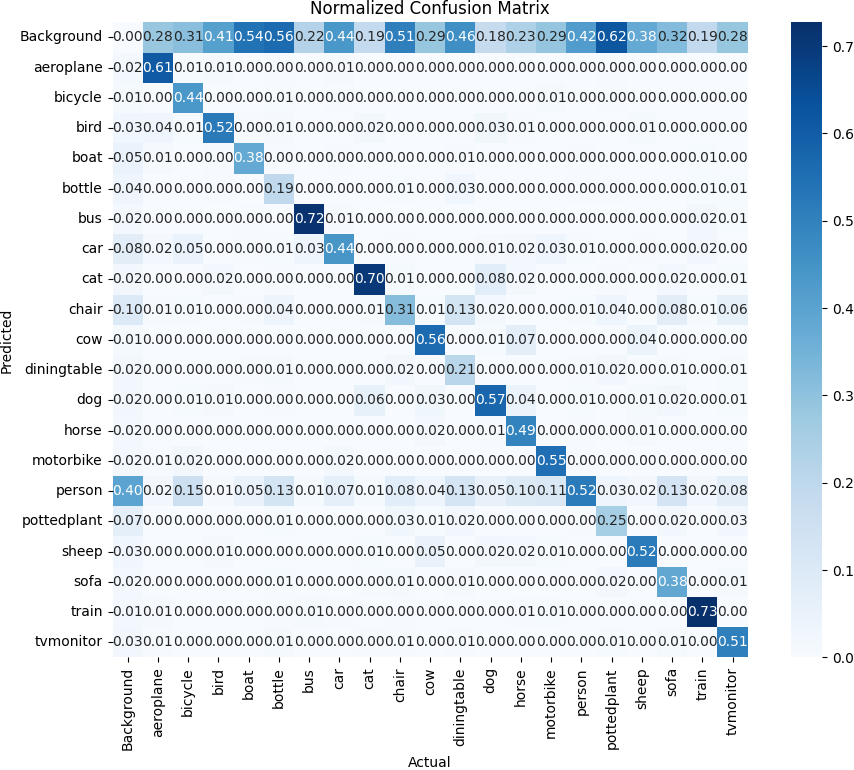
\includegraphics[width=0.7\textwidth]{cm3.png} \\
    \small (a) \\
    \addlinespace[1em]
    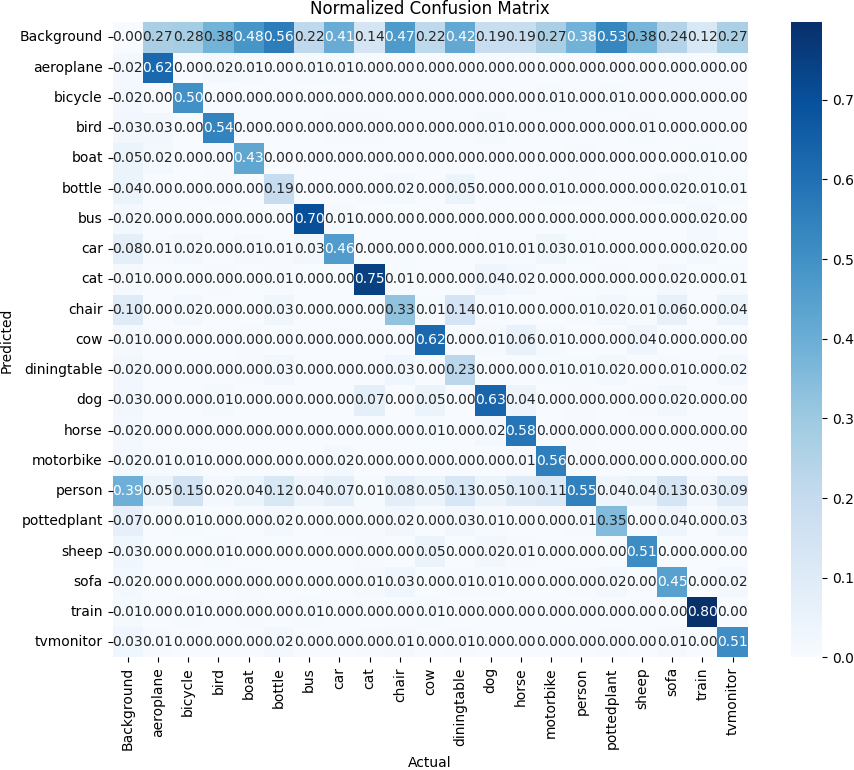
\includegraphics[width=0.7\textwidth]{cm4.png} \\
     \small (b) \\
  \end{tabular}
  \caption{Normalised confusion matrices for multi-label detection of 20 object classes on the Pascal VOC 2012 dataset, using the best-performing models of the SSDLite architecture: (a) baseline model, (b) student model.}
  \label{fig:cm_pascal_voc}
\end{figure}

The student model shows some improvement. Its confusion matrix presents clearer diagonal lines across most categories, indicating more accurate predictions. There are also fewer unclassified examples overall. The classes most reliably identified by the student model are \textit{Train}, \textit{Cat}, and \textit{Bus}. These appear to be among the simpler categories to detect, likely because they have more distinct and consistent visual features than others.

Building on the earlier comparisons, an additional analysis was undertaken to examine the performance of various teacher models, using the same experimental setup as in the previous tests. The outcomes, detailed in Table~\ref{tab:teacher_model_metrics_pascal_voc}, reflect the detection accuracy achieved by each teacher architecture. Interestingly, Faster \gls{rcnn}, \gls{fcos}, and RetinaNet continued to yield the best results, though their performance metrics were lower than the near-ideal values reported in earlier evaluations.

\begin{table}[!htbp]
    \centering
    \begin{adjustbox}{max width=\textwidth}
    \renewcommand{\arraystretch}{1.5}
    \begin{tabular}{|l|c|c|c|c|c|c|c|c|c|}
        \hline
        \textbf{Model} & \textbf{mAP@50--95} & \textbf{mAP@50} & \textbf{mAP@75} & \textbf{mAR@1} & \textbf{mAR@10} & \textbf{mAR@100} & \textbf{Precision} & \textbf{Recall} & \textbf{F1 Score} \\ \hline \hline
        \textbf{RetinaNet} & 0.77 & 0.86 & 0.79 & 0.60 & 0.81 & 0.81 & 0.26 & 0.90 & 0.38 \\\hline
        \textbf{FCOS} & \textbf{0.80} & 0.88 & \textbf{0.82} & \textbf{0.61} & \textbf{0.84} & \textbf{0.84} & 0.43 & \textbf{0.91} & 0.56 \\\hline
        \textbf{Faster R-CNN} & 0.77 & \textbf{0.91} & \textbf{0.82} & 0.59 & 0.82 & 0.82 & \textbf{0.56} & \textbf{0.91} & \textbf{0.68} \\\hline
        \textbf{SSD} & 0.42 & 0.56 & 0.49 & 0.41 & 0.48 & 0.48 & 0.25 & 0.69 & 0.36 \\\hline
        \textbf{SSDLite} & 0.49 & 0.61 & 0.54 & 0.46 & 0.55 & 0.55 & 0.04 & 0.79 & 0.07 \\
        \hline
    \end{tabular}
    \renewcommand{\arraystretch}{1}
    \end{adjustbox}
    \caption{Comparison of teacher model performance across key detection metrics, trained on the Pascal VOC 2012 dataset for multi-label detection of 20 object classes.}
    \label{tab:teacher_model_metrics_pascal_voc}
\end{table}

A notable observation is that, despite their weaker performance as teacher models, both \gls{ssd} and SSDLite produced relatively strong student models. This outcome contrasts with RetinaNet and \gls{fcos}, which, despite achieving better detection scores as teacher models, produced less accurate student versions.

\gls{fcos}, in particular, stood out as a strong teacher, closely following Faster \gls{rcnn} and even outperforming it in some metrics. A consistent pattern across all teacher models was the high recall values, while precision scores showed greater variation. SSDLite, in this context, had the lowest precision, whereas the other models achieved values between 0.25 and 0.56. These figures were somewhat lower than anticipated, especially considering the use of privileged information. The results also suggest that increasing the number of classes introduces added complexity, which negatively affects both teacher and student performance across all detection metrics.

The training times for all models used in this experiment are presented in Figure~\ref{fig:pascal_voc_training_time}. Compared to earlier experiments, these models generally required less time to train. Notably, most models in this study exhibited a more uniform rate of convergence, in contrast to the more varied patterns seen in earlier experiments.

\begin{figure}[!ht]
    \centering
    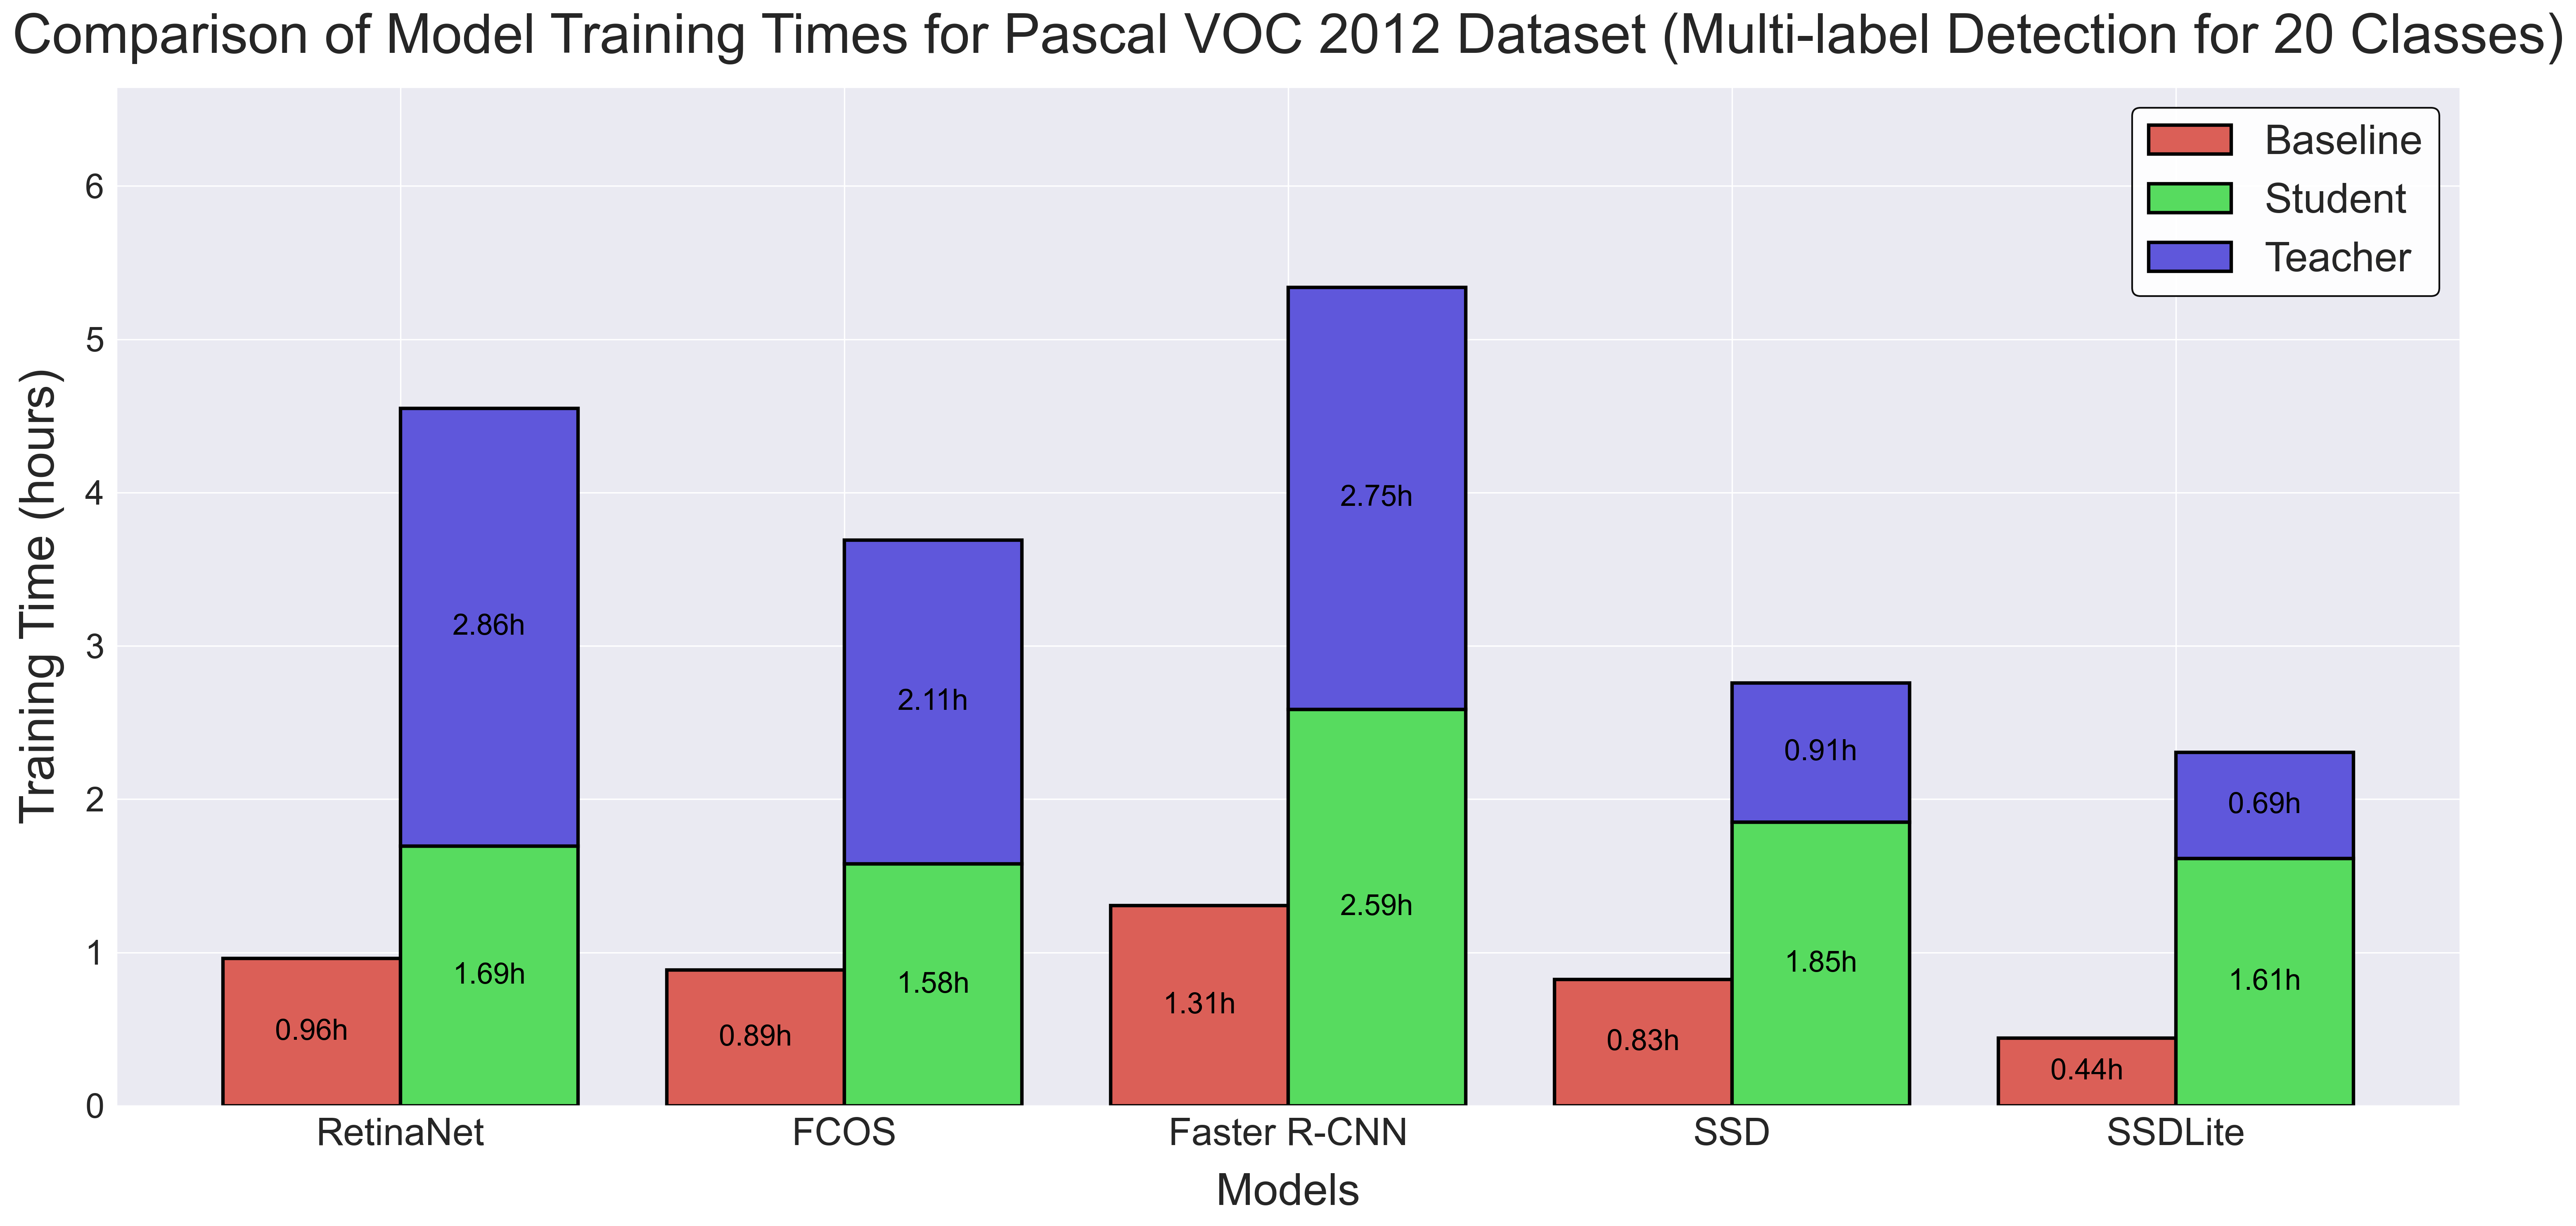
\includegraphics[width=1\textwidth]{training_times_pascal_voc_2012_dataset_multi_label_detection_for_20_classes.png}
    \caption{Comparison of model training times on the Pascal VOC 2012 dataset for multi-label detection of 20 object classes.}
    \label{fig:pascal_voc_training_time}
\end{figure}

RetinaNet and Faster \gls{rcnn} had the longest training times for their student models. On the other hand, \gls{ssd} and SSDLite, which completed training more quickly, produced the strongest student performances in this experiment. Across all models, student training took longer than the corresponding baselines, while teacher models consistently required the most time overall.

A comparison of model sizes, as detailed in Table~\ref{tab:model_configs_pascal_voc}, reveals some differences from the findings of previous experiments. The models in this study now feature more parameters and a larger overall size, primarily due to the increased number of classes to 20. This expansion requires additional parameters in the prediction head, which in turn increases the total model size.

\begin{table}[!ht]
    \centering
    \begin{tabular}{llcc}
        \toprule
        \textbf{Model Configuration} & \textbf{Type} & \textbf{Size (MB)} & \textbf{Parameters (M)} \\
        \midrule
        \multirow{5}{*}{\textbf{Baseline}} 
            & RetinaNet     & 124.22 & 32.56 \\
            & FCOS          & 122.48 & 32.11 \\
            & Faster R-CNN  & 157.92 & 41.40 \\
            & SSD           & 100.27 & 26.29 \\
            & SSDLite       & 9.42   & 2.47 \\
        \midrule
        \multirow{5}{*}{\textbf{Student}} 
            & RetinaNet     & 124.22 & 32.56 \\
            & FCOS          & 122.48 & 32.11 \\
            & Faster R-CNN  & 157.92 & 41.40 \\
            & SSD           & 100.27 & 26.29 \\
            & SSDLite       & 9.42   & 2.47 \\
        \bottomrule
    \end{tabular}
    \caption{Comparison of model configurations for trained baseline and student models on the Pascal VOC 2012 dataset for multi-label object detection, including model type, size in megabytes, and number of parameters (in millions).}
    \label{tab:model_configs_pascal_voc}
\end{table}

Despite this growth, the results demonstrate that applying the proposed methodology to any detector leads to improved detection accuracy. Importantly, this improvement is realised without relying on more complex or computationally intensive architectures. Through various experimental setups, each conducted with strict controls and repeated testing, the method consistently delivered better performance while keeping both model size and parameter count under control.


\section{Ablation Study on the Alpha Parameter}
\label{sec:5_alpha_exp}
% Glorja lil Missier, lil Iben u lil Ispirtu s-Santu, Kif kien mill bidu, issa u dejjem ghal dejjem. Amen. Grazzi

An ablation study was conducted to evaluate the effect of the \gls{alpha} parameter, which determines the importance given to the teacher network when distilling knowledge to the student model. Following the approach outlined in \cite{lab2wild}, various \gls{alpha} values were explored: 0, 0.25, 0.5, 0.75, and 1. The results of this study, presented in Figures~\ref{fig:ablation_combined} and \ref{fig:ablation_combined2}, assess which \gls{alpha} value best supports the distillation process. This figure compares the outcomes of both the within-dataset experiments and the models trained on the Pascal \gls{voc} 2012 dataset.

\begin{figure}[!ht]
    \centering
    \begin{tabular}{c}
        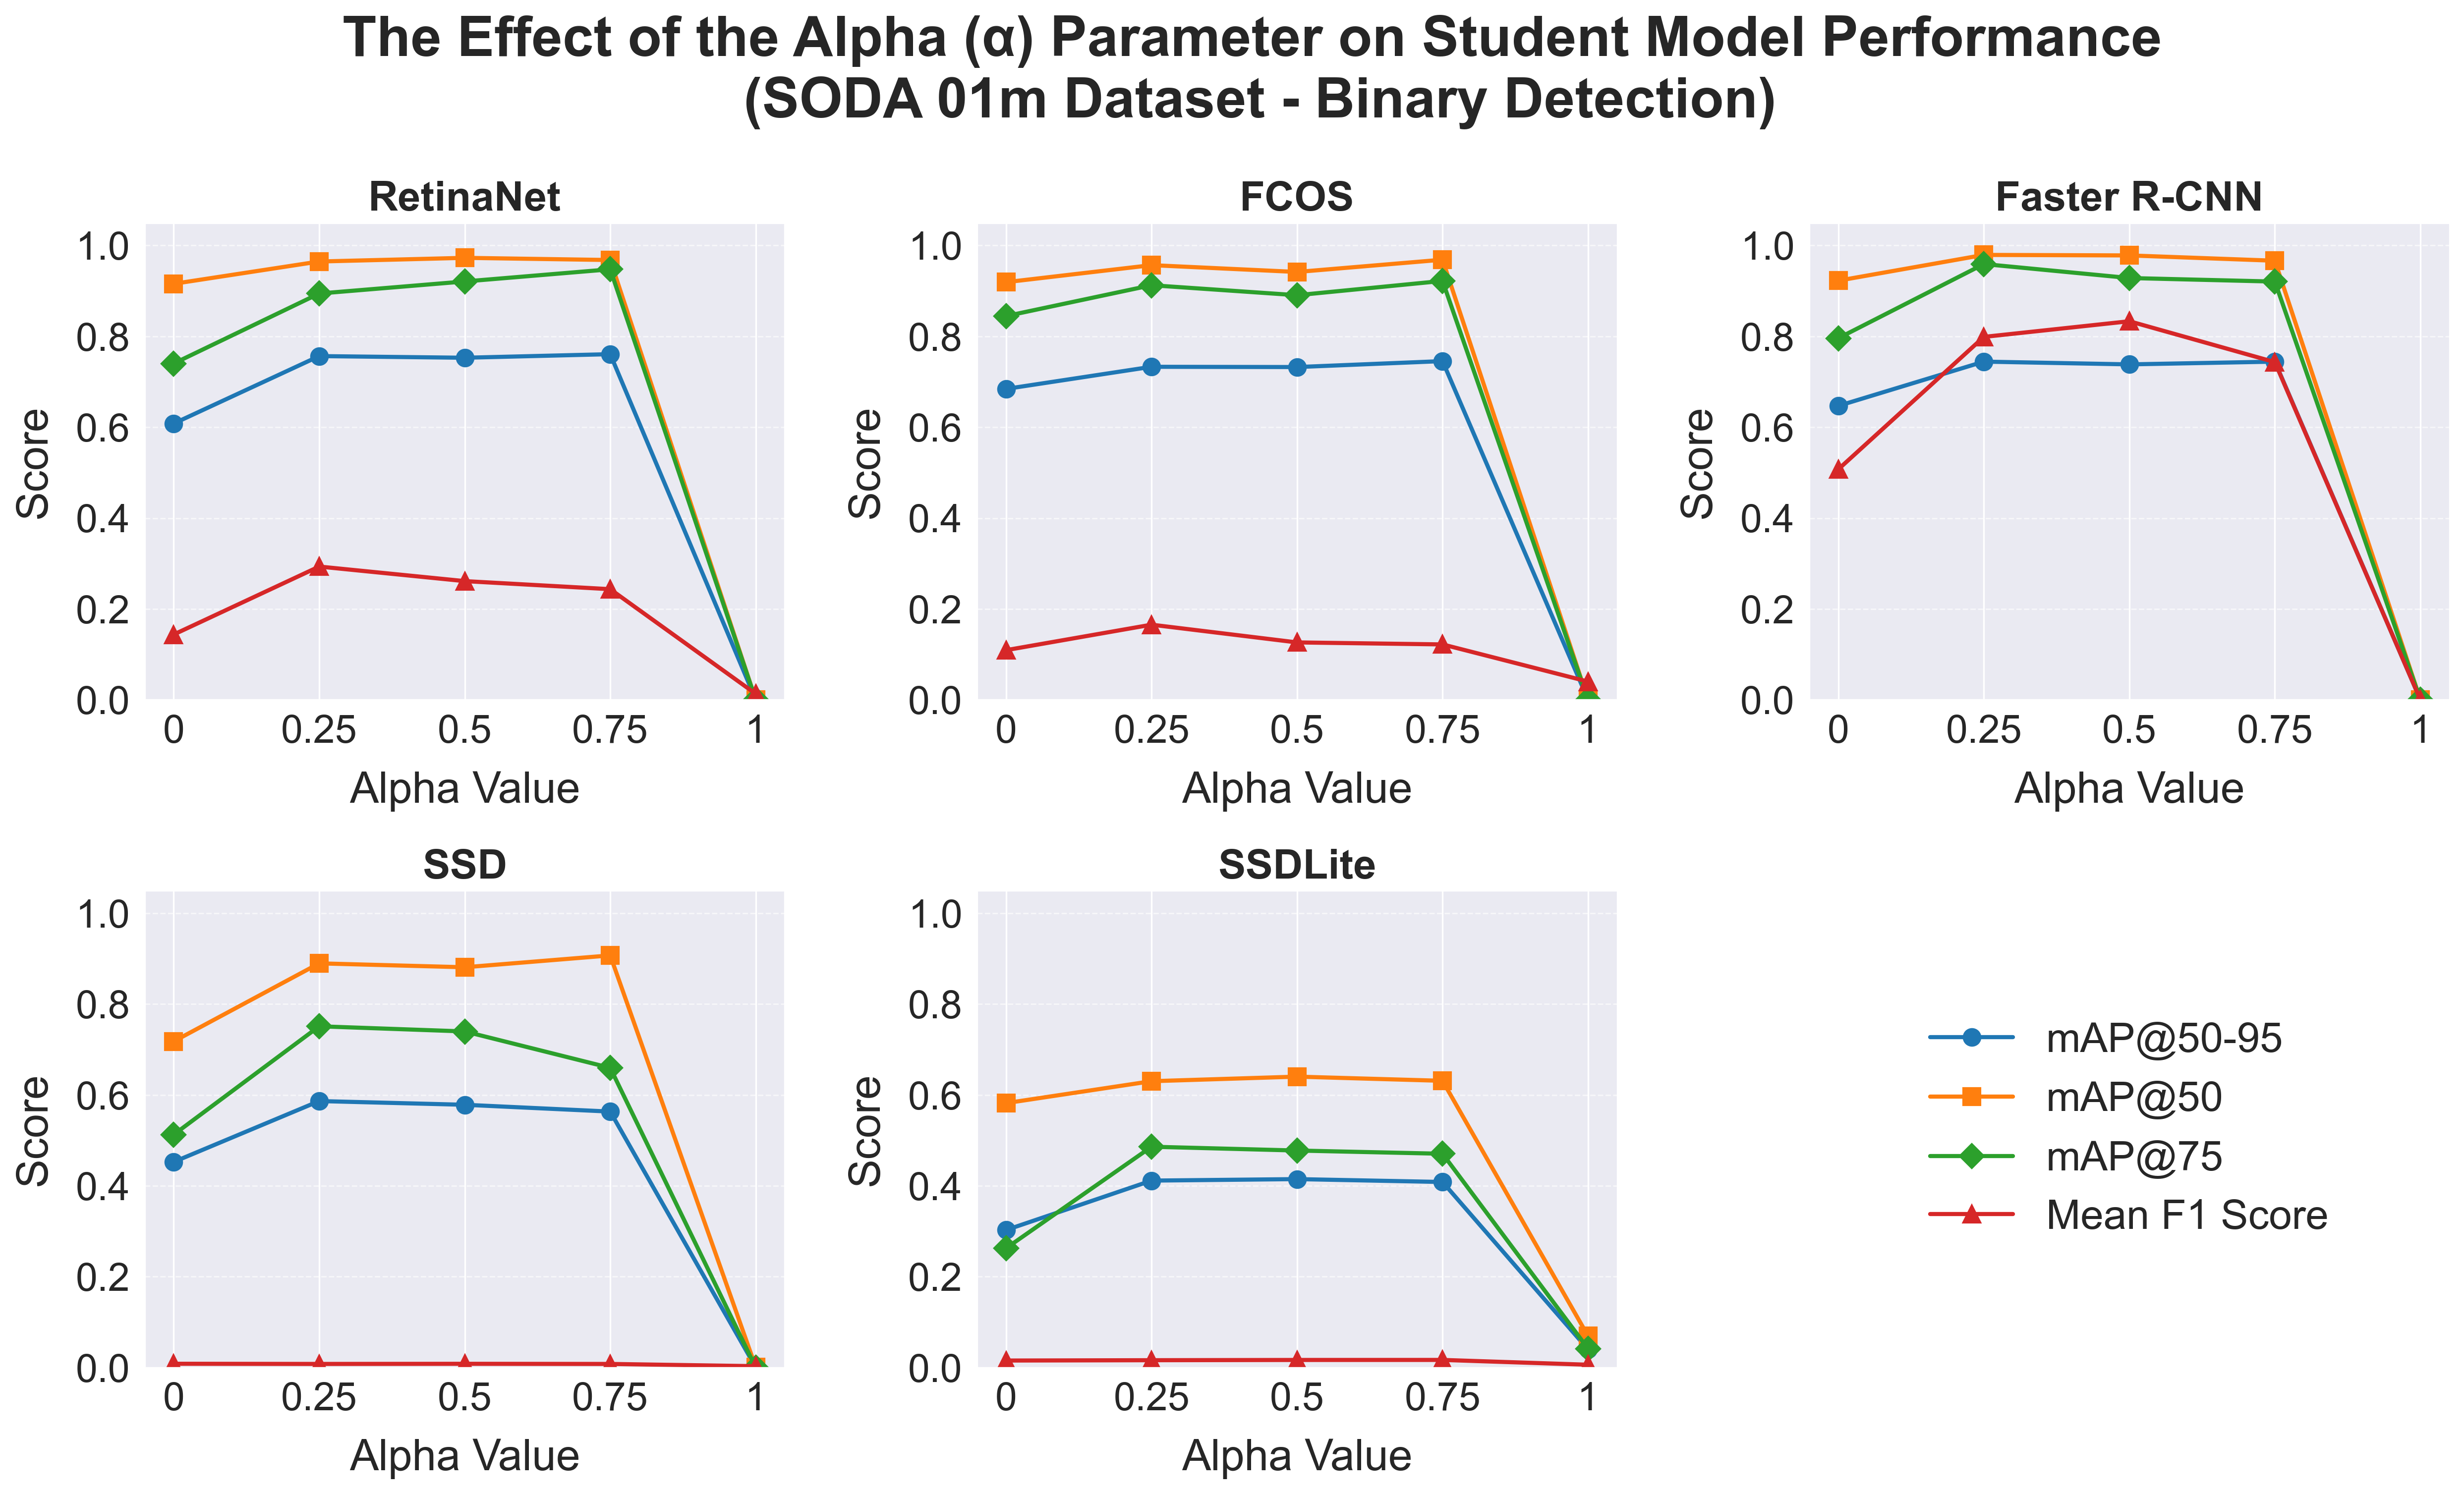
\includegraphics[width=0.9\textwidth]{ablation_study_soda_01m.png} \\
        \small (a) \\
        \addlinespace[1em]
        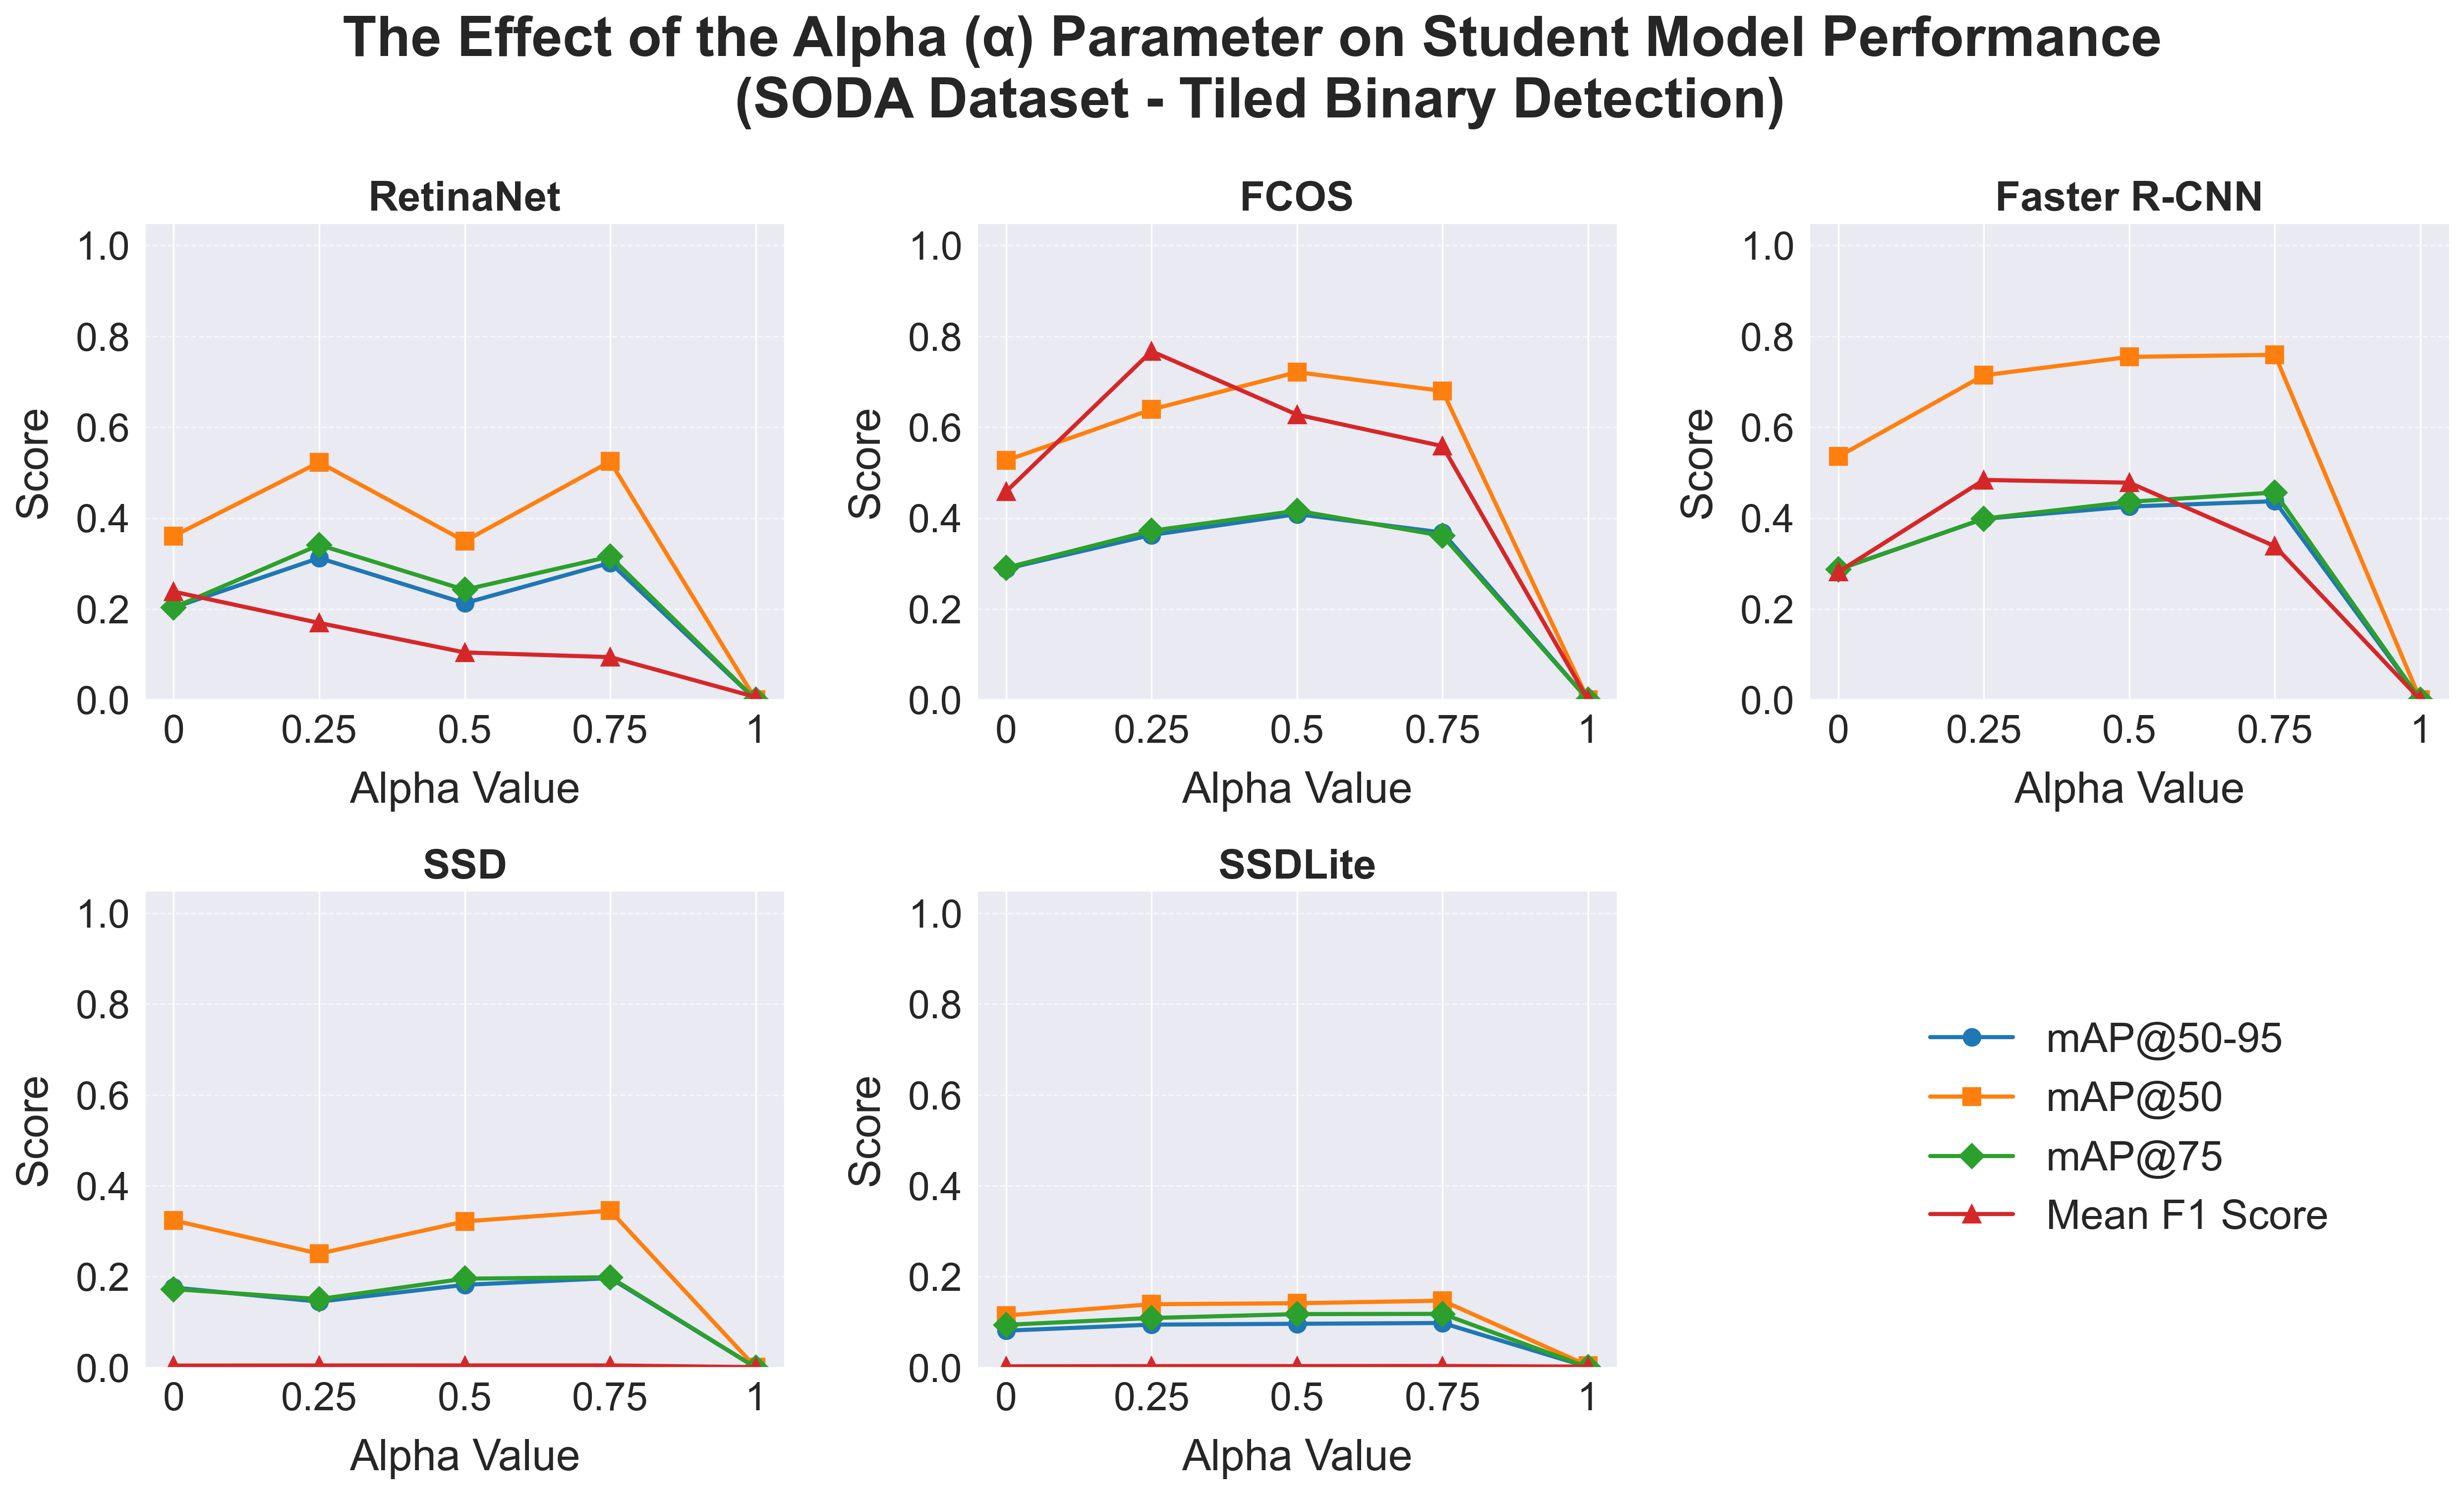
\includegraphics[width=0.9\textwidth]{ablation_study_soda_tiled_single.png} \\
        \small (b) \\
    \end{tabular}
    \caption{Assessing the impact of the alpha (\gls{alpha}) parameter on student model performance. 
    (a) shows results for the \gls{soda} dataset at a 1-metre altitude for binary litter detection, while 
    (b) presents results on the 3$\times$3 tiled \gls{soda} dataset across all altitudes for binary litter detection.}
    \label{fig:ablation_combined}
\end{figure}

\begin{figure}[!ht]
    \centering
    \begin{tabular}{c}
        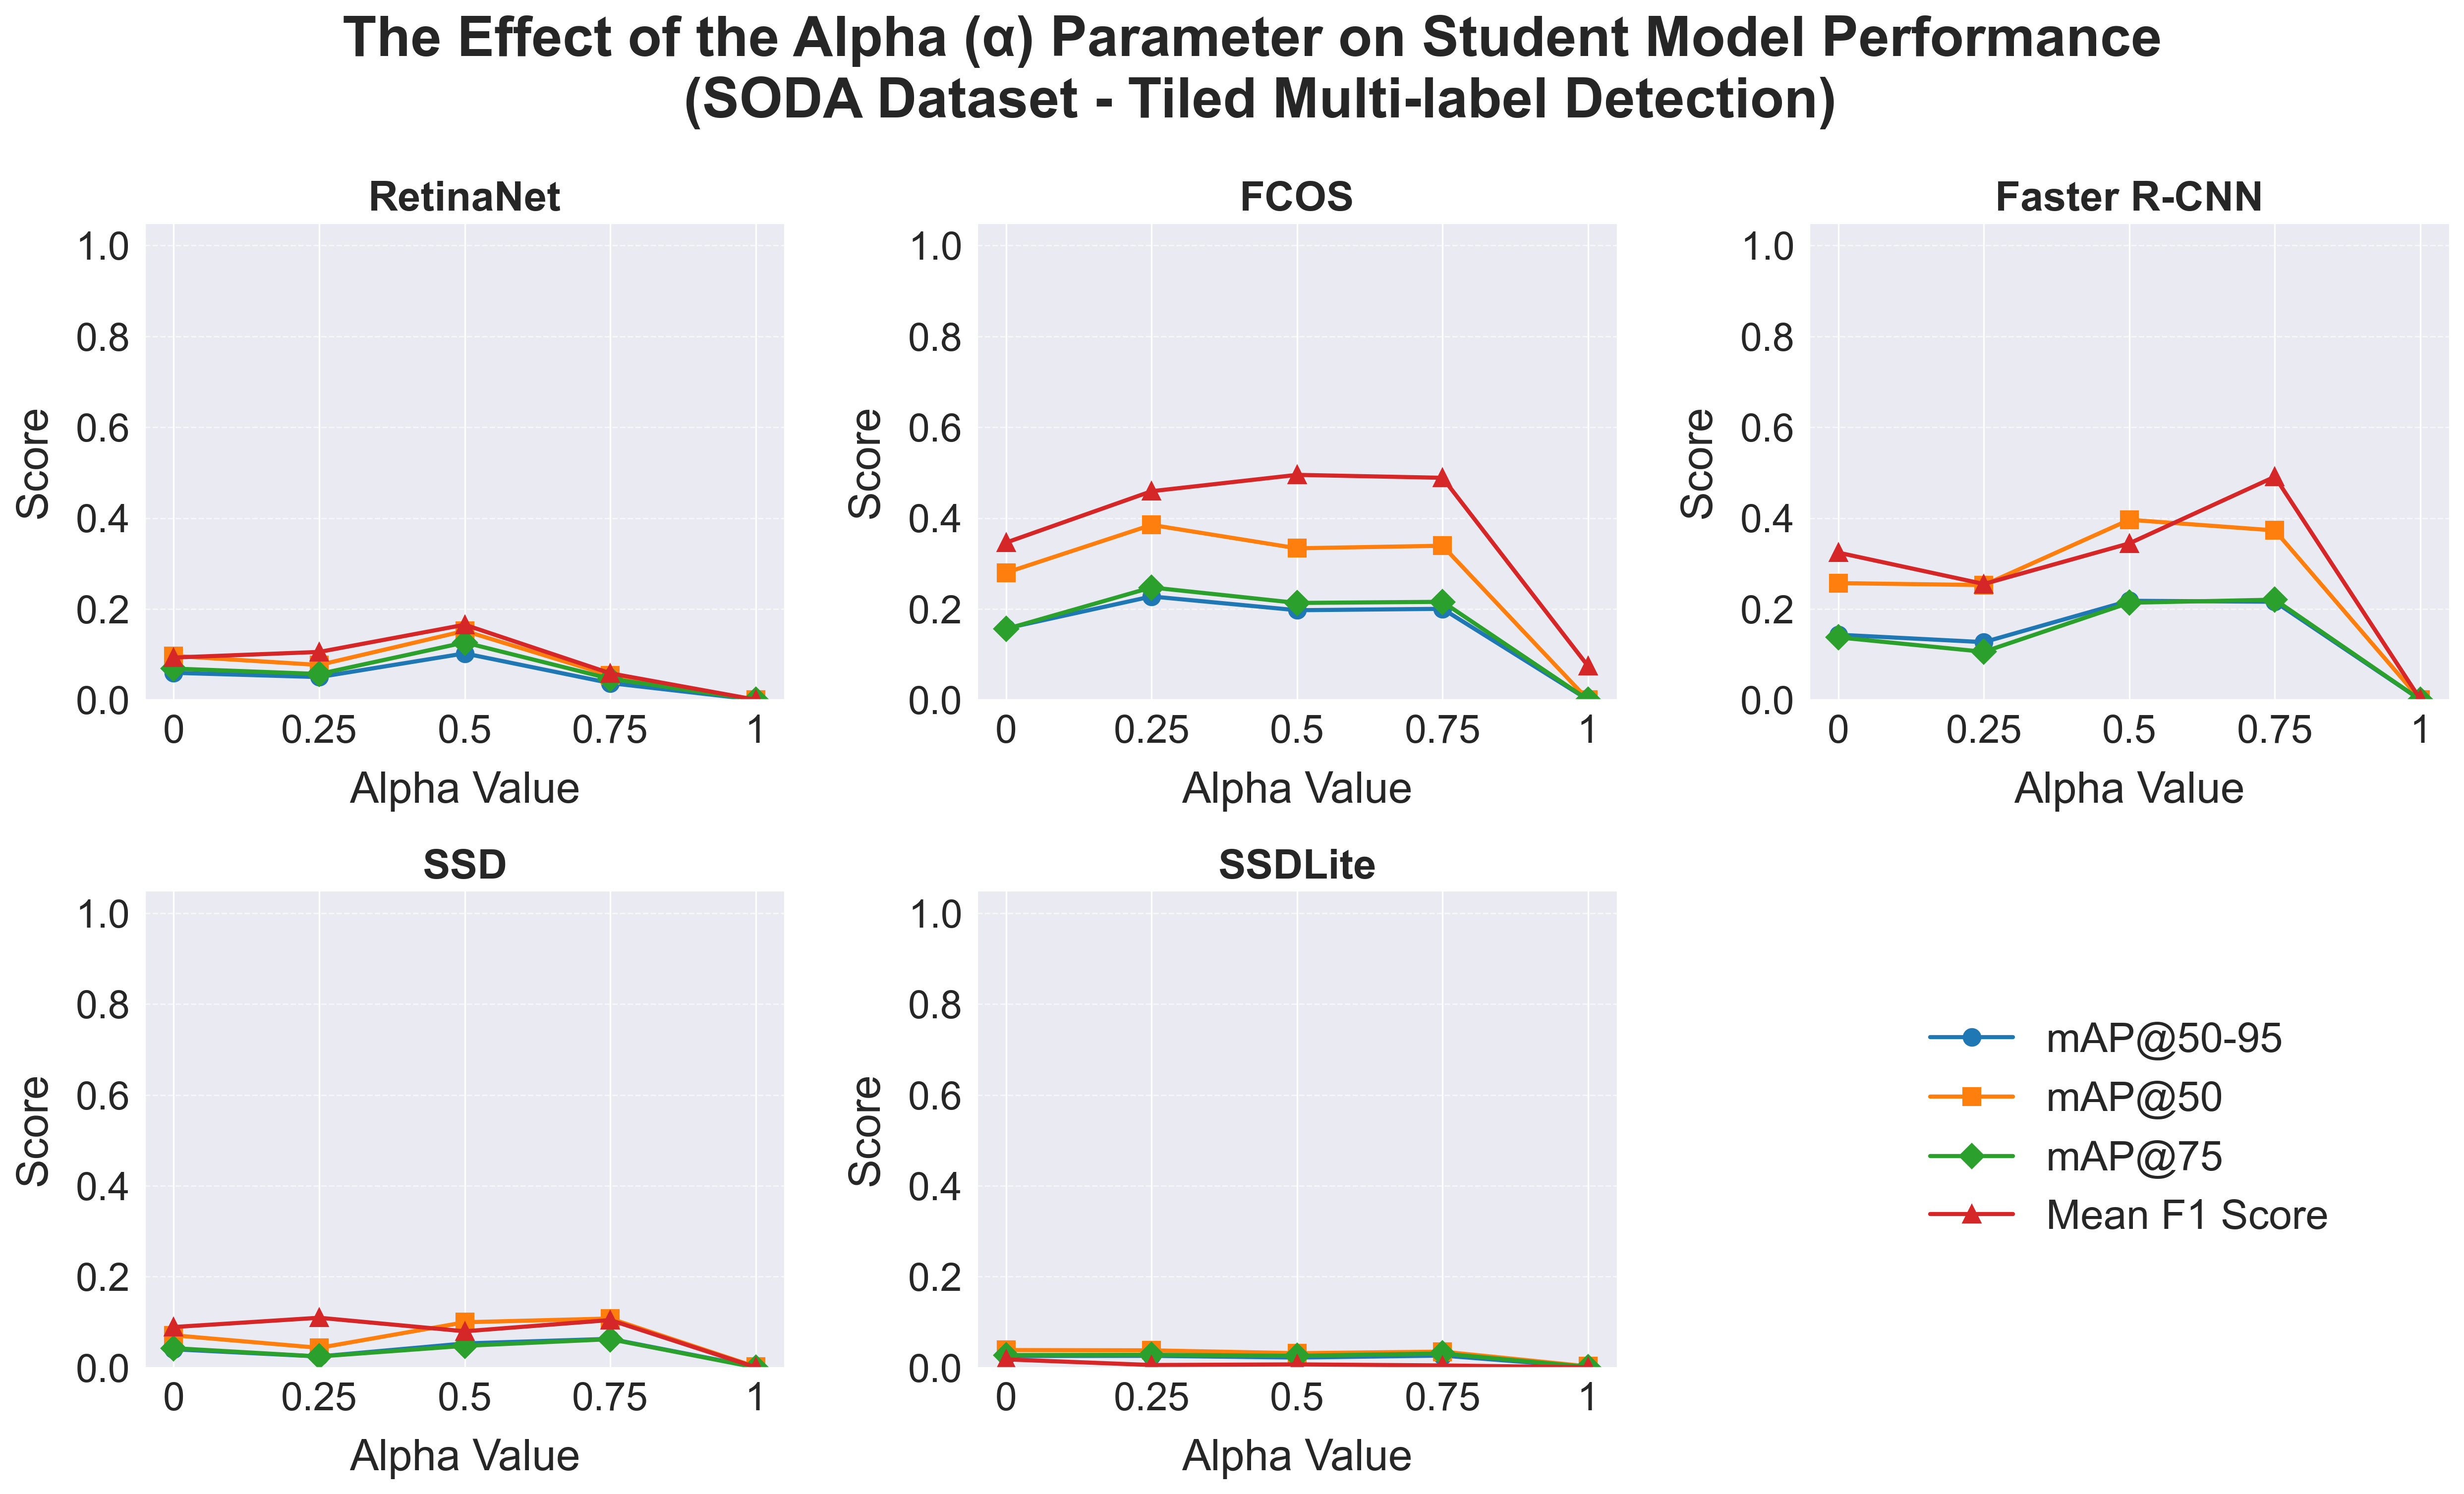
\includegraphics[width=0.9\textwidth]{ablation_study.png} \\
        \small (a) \\
        \addlinespace[1em]
        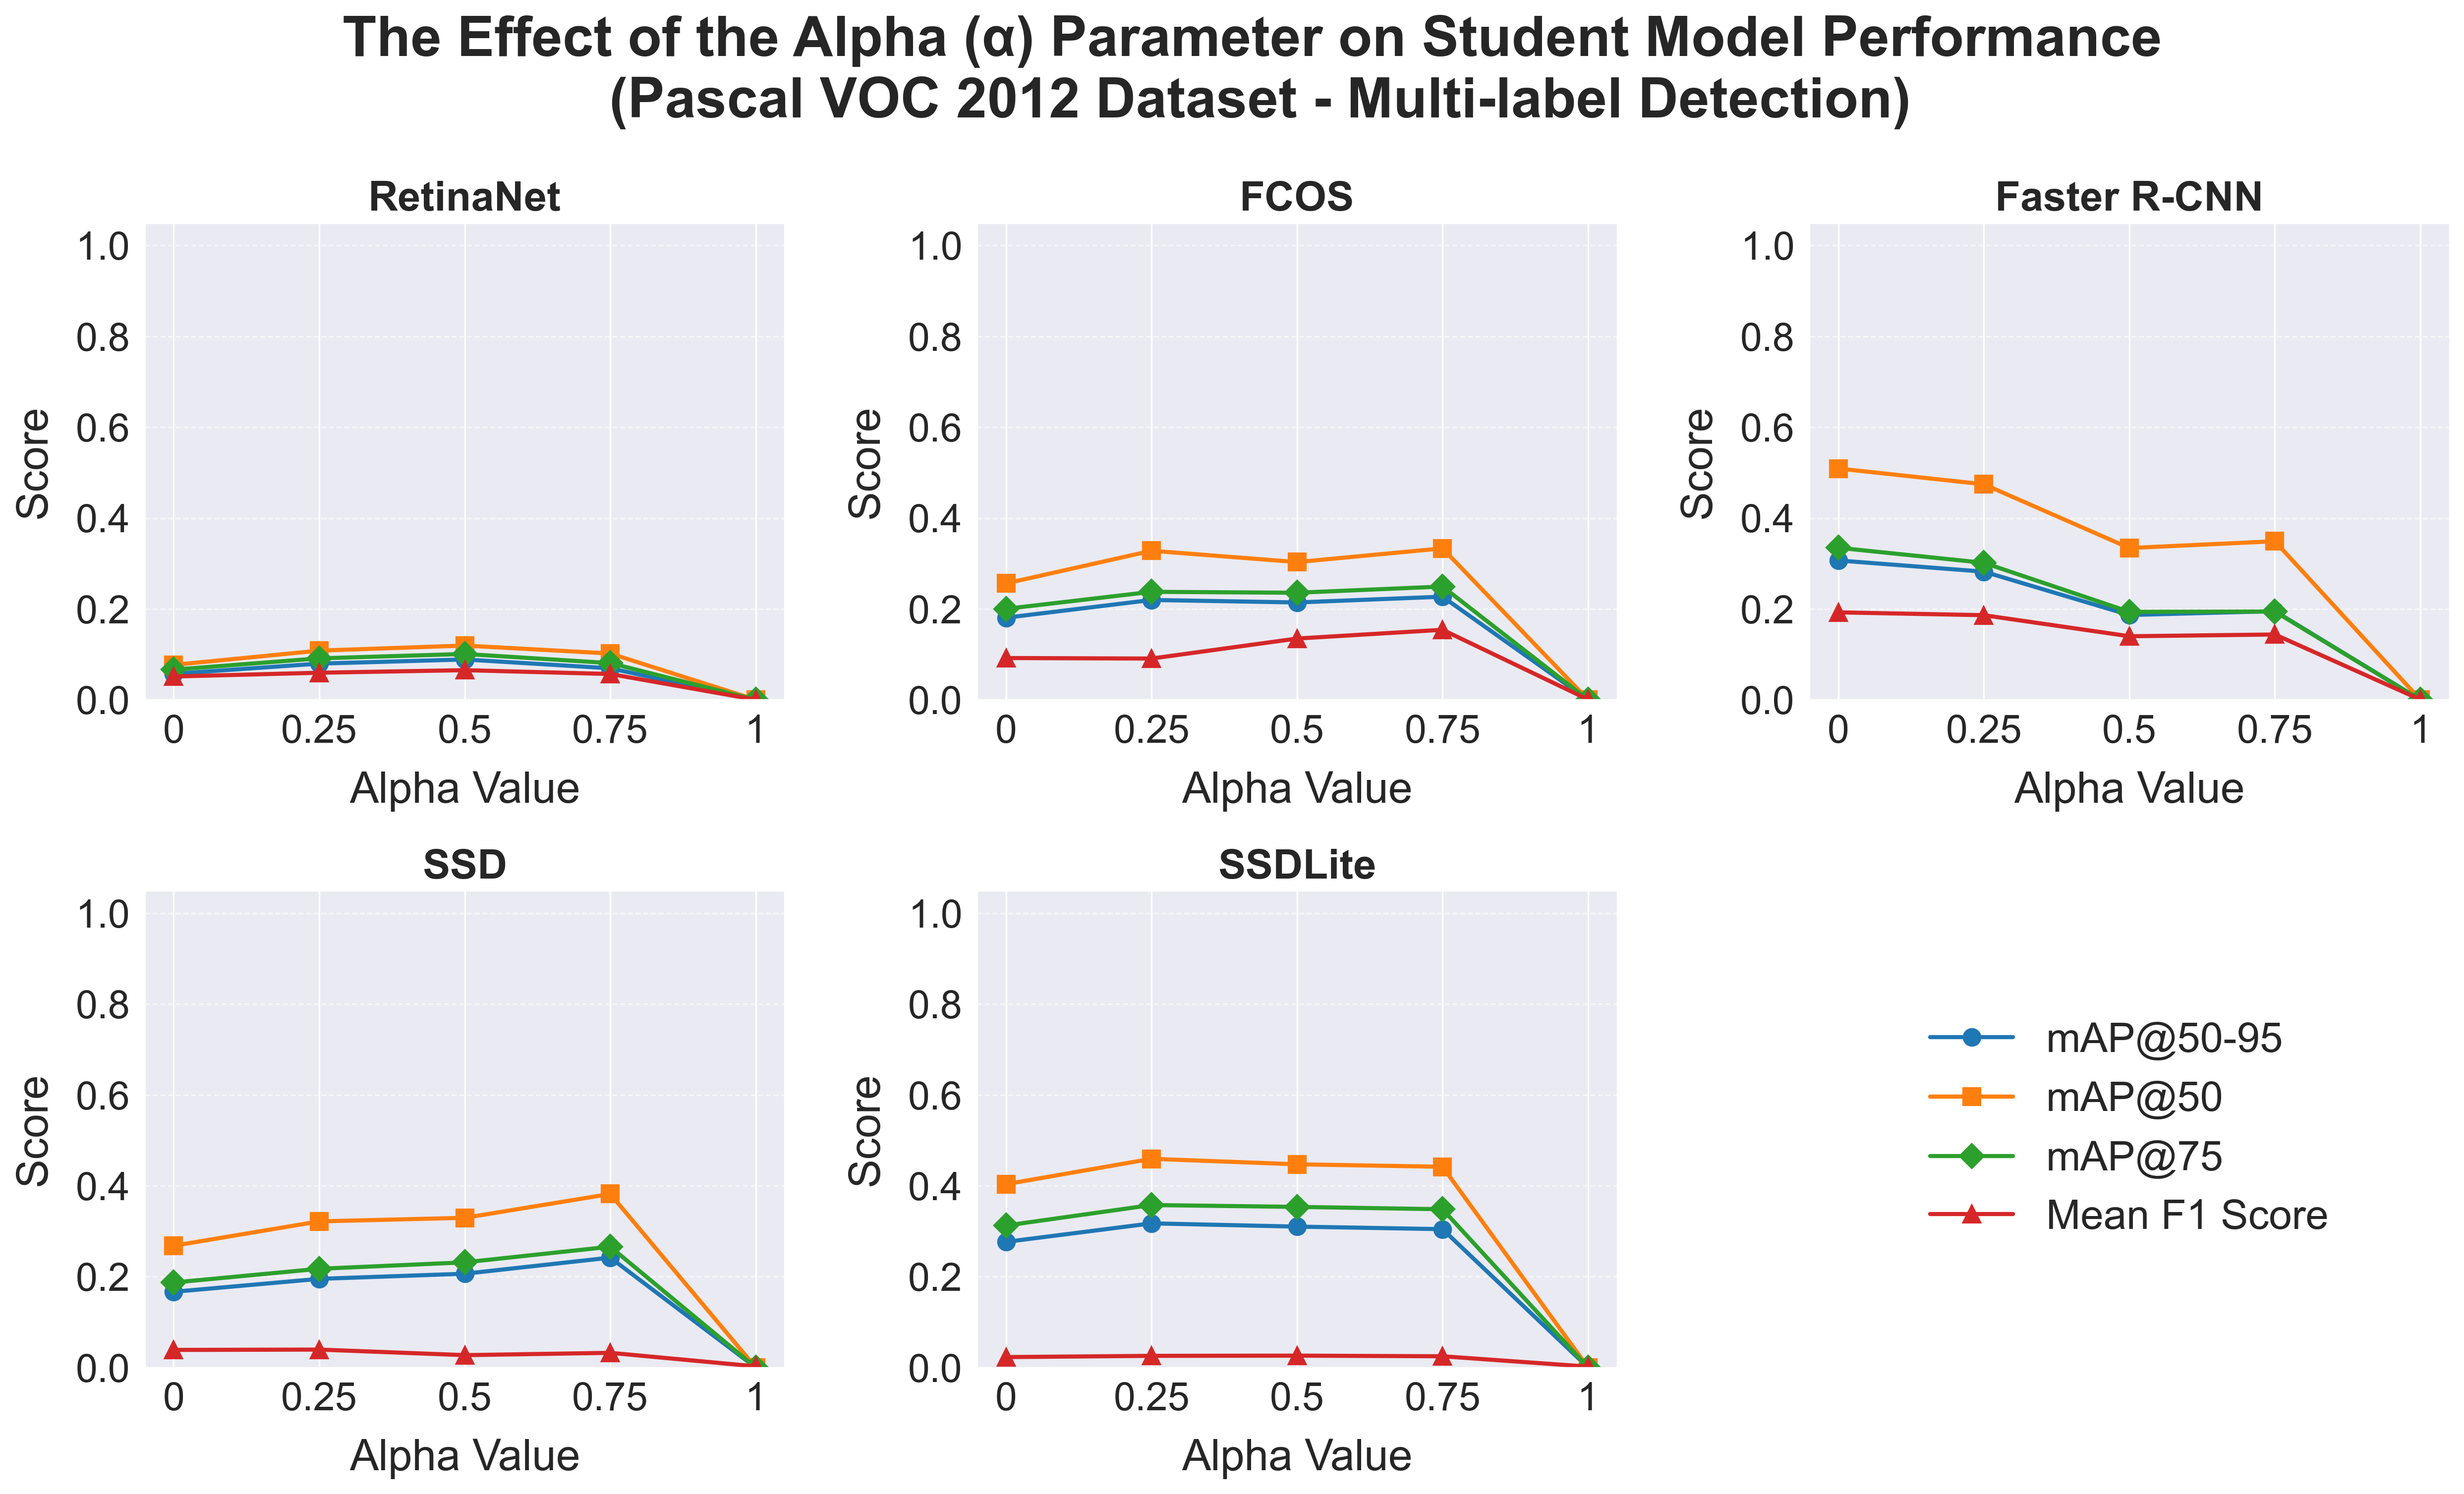
\includegraphics[width=0.9\textwidth]{ablation_study_pascal_voc.png} \\
        \small (b) \\
    \end{tabular}
    \caption{Assessing the impact of the alpha (\gls{alpha}) parameter on student model performance. 
    (a) shows results on the 3$\times$3 tiled \gls{soda} dataset across all altitudes for multi-label litter detection, while 
    (b) presents results on the Pascal \gls{voc} 2012 dataset for multi-label object detection.}
    \label{fig:ablation_combined2}
\end{figure}

The principal finding from this analysis is that, across all experiments, the most effective performance in terms of the primary object detection metric (\gls{map}@50–95) was observed when \gls{alpha} values were set between 0.25 and 0.5. There were a few isolated instances in which a value of 0.75 produced comparable results, but these were exceptions rather than the norm. In general, when \gls{alpha} was set to 1, which gives full control to the teacher, all metrics showed near-zero scores. For F1 scores, the trend for achieving high object classification performance was observed at \gls{alpha} values of 0.25 and 0.5. However, there were a few exceptions in the multi-label litter detection experiment, where \gls{fcos} and Faster \gls{rcnn} favoured \gls{alpha} = 0.75. 

Further analysis revealed that for RetinaNet, on average, \gls{alpha} values of 0.5 and 0.75 yielded the best results, while for \gls{fcos}, the optimal values for \gls{map}@50, \gls{map}@75, and F1 scores were similar, with \gls{alpha} = 0.25 being optimal for the harder metric, \gls{map}@70–95. For Faster \gls{rcnn} and \gls{ssd}, which followed a similar trend, \gls{alpha} values between 0.5 and 0.75 delivered the best results. Finally, for SSDLite, \gls{alpha} = 0.5 appeared to be the most effective configuration. That said, this architecture generally delivered weak results across all metrics in the litter detection experiments. However, it did show a modest yet meaningful improvement in the Pascal \gls{voc} 2012 evaluation.

Thus, the findings of this ablation study indicate that setting the \gls{alpha} parameter between 0.25 and 0.5 for the proposed approach provides the most consistent and effective results across the detection metrics. Employing these values provides the teacher enough say to help without overwhelming the student. When the teacher’s influence was set to the maximum (\gls{alpha} = 1), performance dropped sharply, showing that too much reliance on the teacher can hold the student back. Although the results align with those presented in \cite{lab2wild}, tuning \gls{alpha} based on the particular task is still necessary. Some models, for instance, performed better on the litter detection tasks when \gls{alpha} was set to 0.75, while the same models reached their best performance on Pascal \gls{voc} 2012 with a value of 0.25. The appropriate value depends on the nature of the data and the specific problem being addressed.


\section{Visual Comparison of Model Predictions}
\label{sec:5_visual_results}
% Glorja lil Missier, u lil Iben u lil Ispirtu s-Santu, Kif kien mill bidu issa u ghal dejjem ta' dejjem. Amen. Grazzi

In addition to the evaluation outlined in the previous experiments, which is based on established object detection metrics, it is equally valuable to consider whether improvements can be observed visually through the integration of \gls{lupi} using the proposed methodology. This form of comparison helps to assess whether the predictions are qualitatively better. To address this, the following section presents visual results across the various experiments, comparing outputs from both within- and across-dataset models, as well as from those trained on the Pascal \gls{voc} 2012 dataset. The aim is to compare the visual predictions from the best-performing baseline and student models of the same architecture type, using sample images taken from the test sets of each dataset. The corresponding results are illustrated in Figures \ref{fig:visuals_soda}, \ref{fig:visuals_bdw}, \ref{fig:visuals_uavvaste}, and \ref{fig:visuals_pascal_voc}.

\begin{figure}[!ht]
  \centering
  \begin{tabular}{cc}
    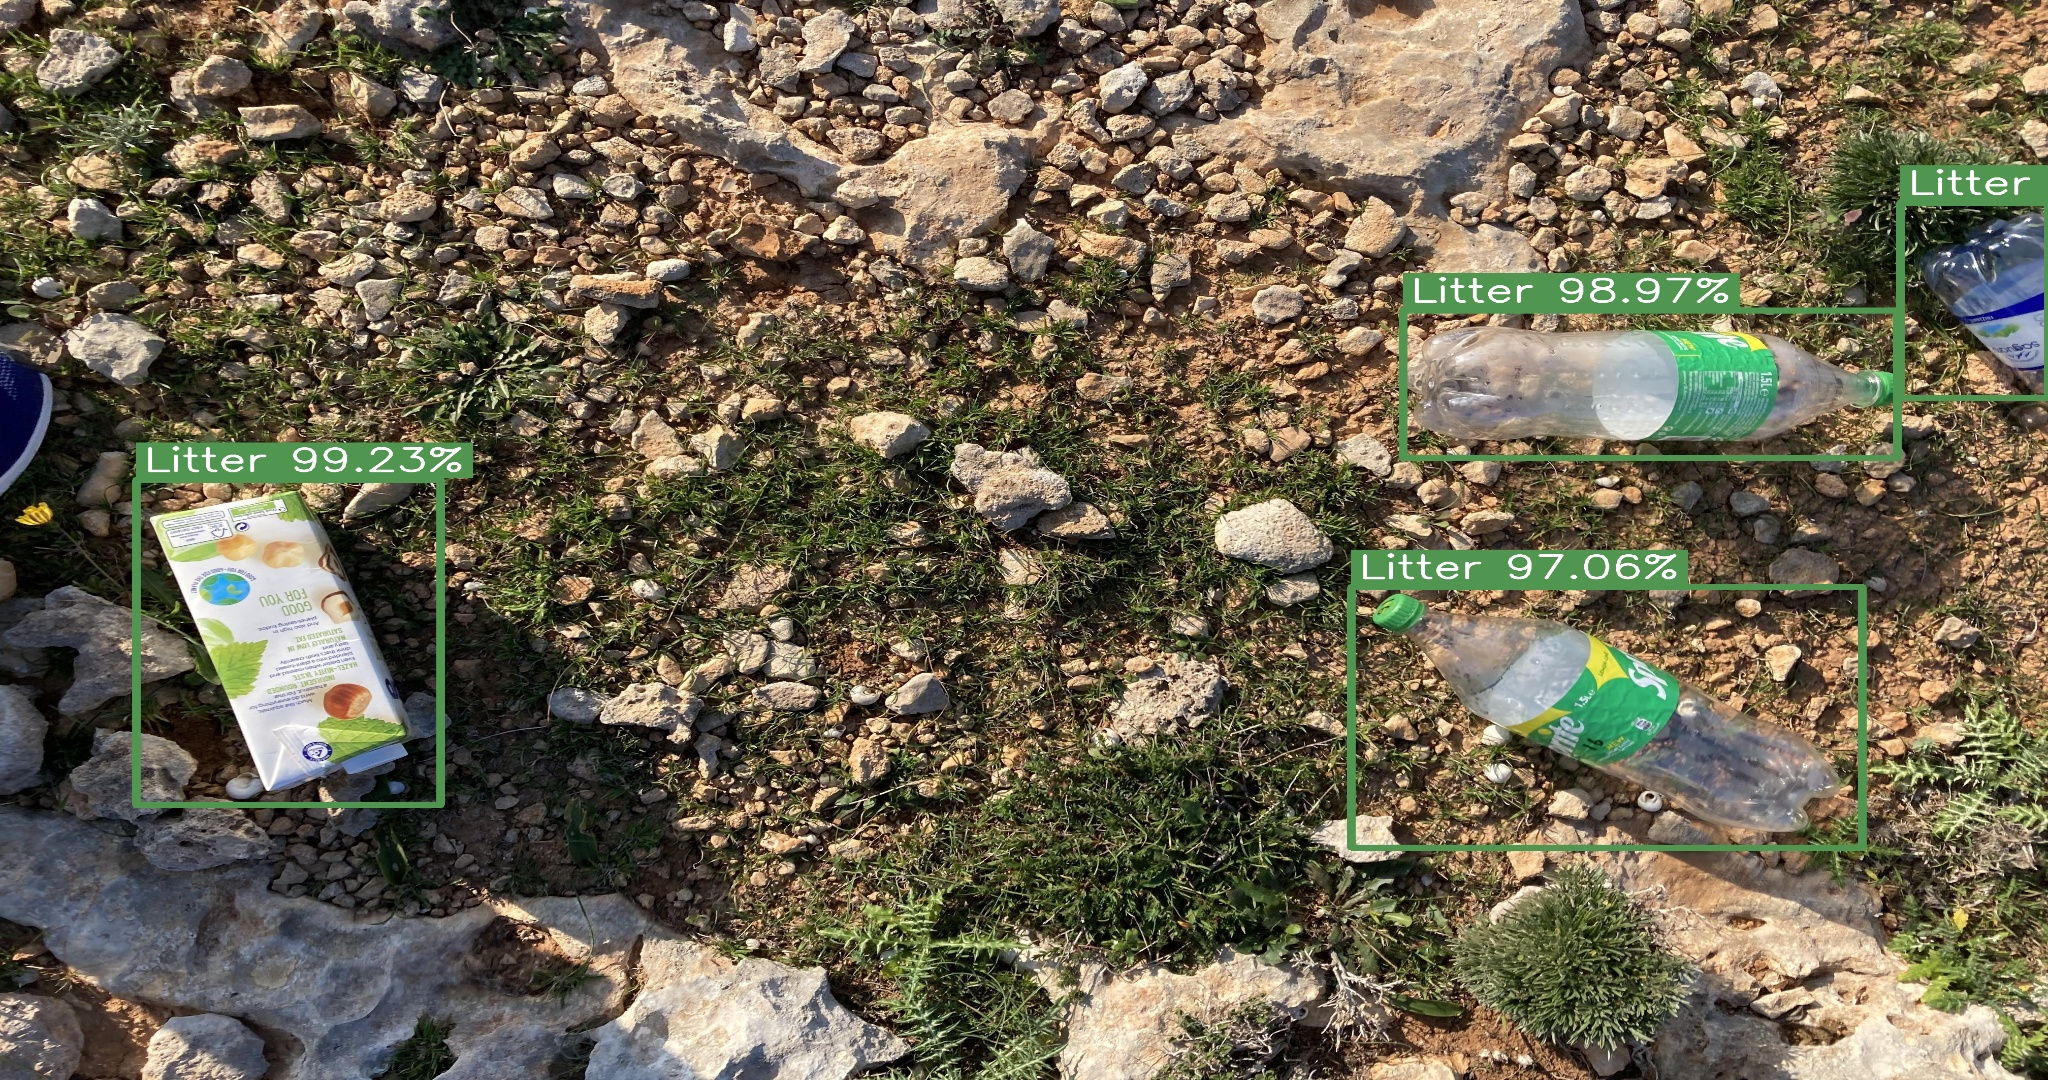
\includegraphics[width=0.47\textwidth]{visual1.jpg} &
    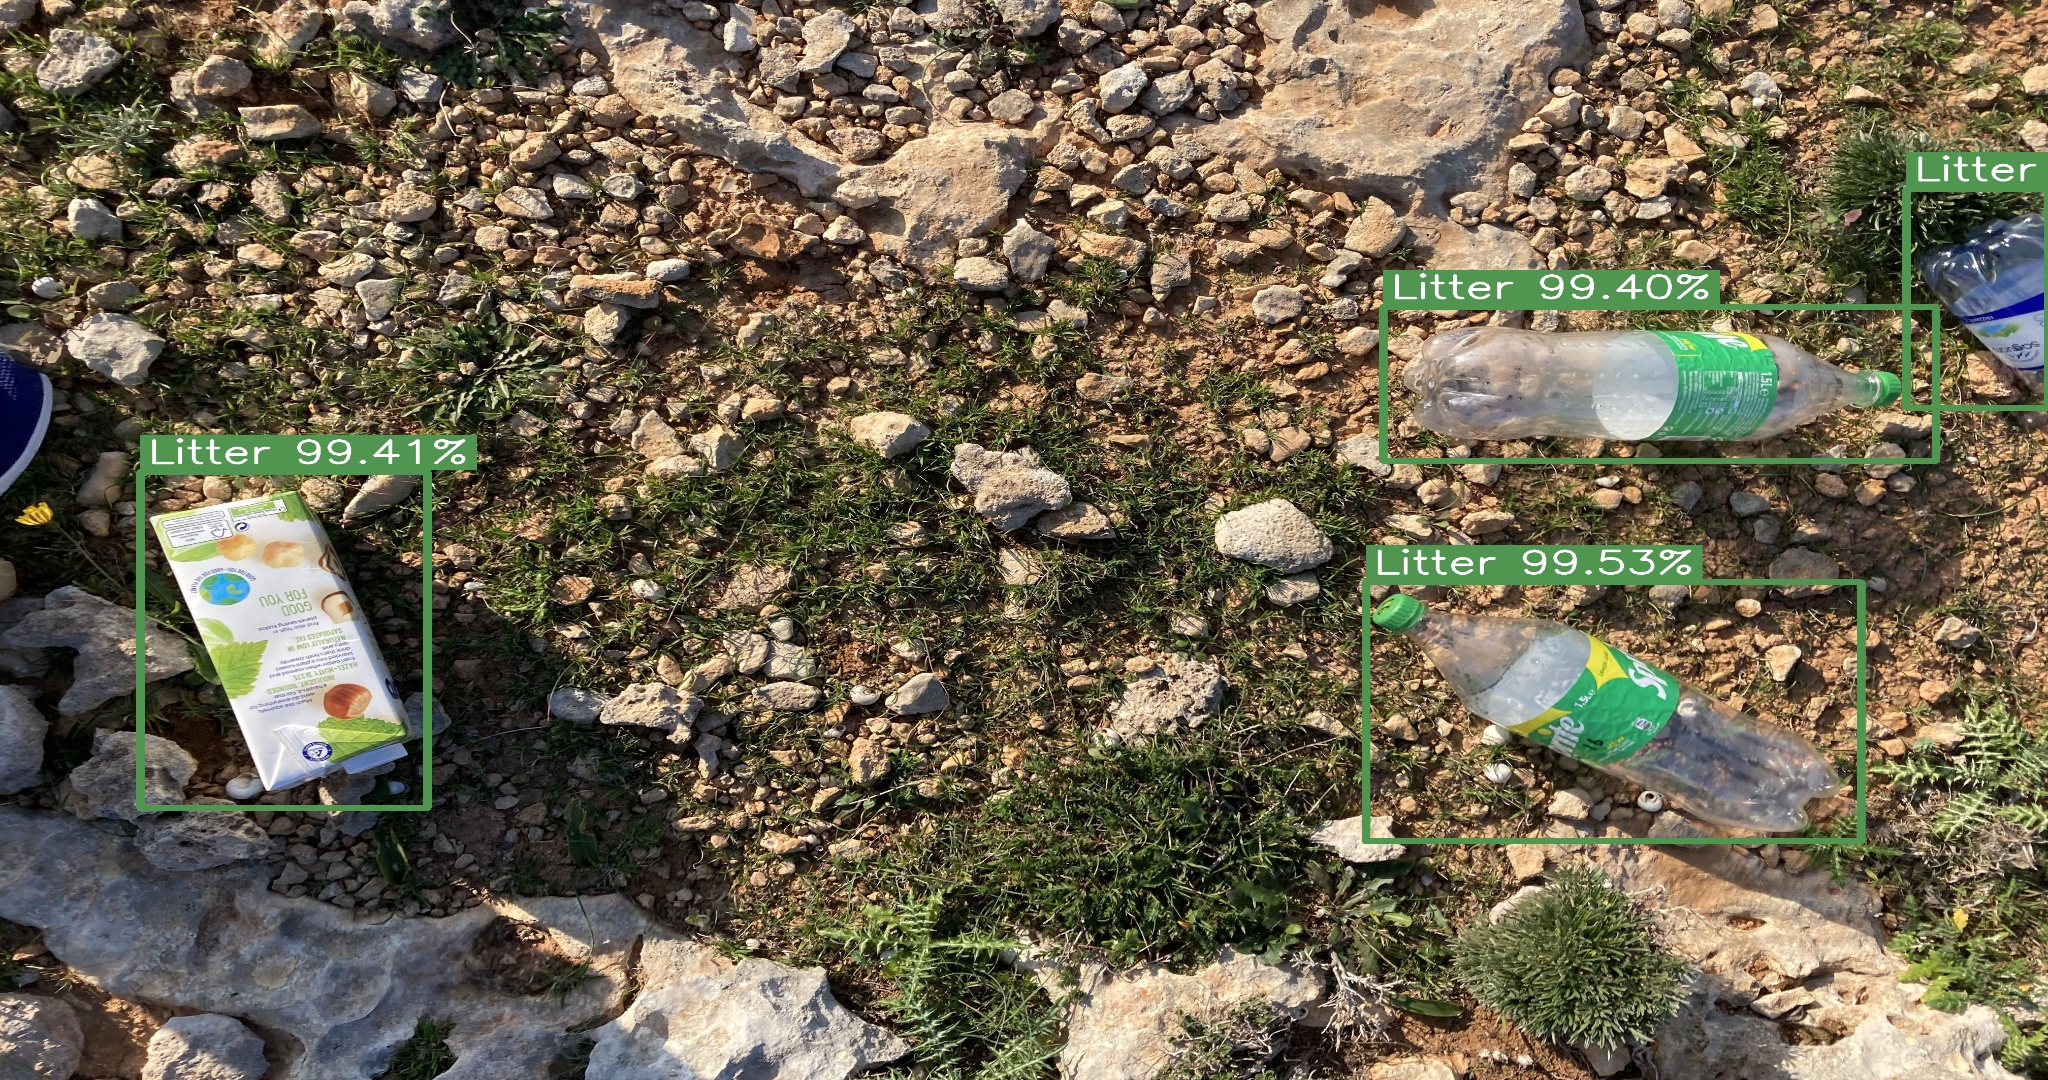
\includegraphics[width=0.47\textwidth]{visual2.jpg} \\
    \small (a) & \small (b) \\
    \addlinespace[1em]
    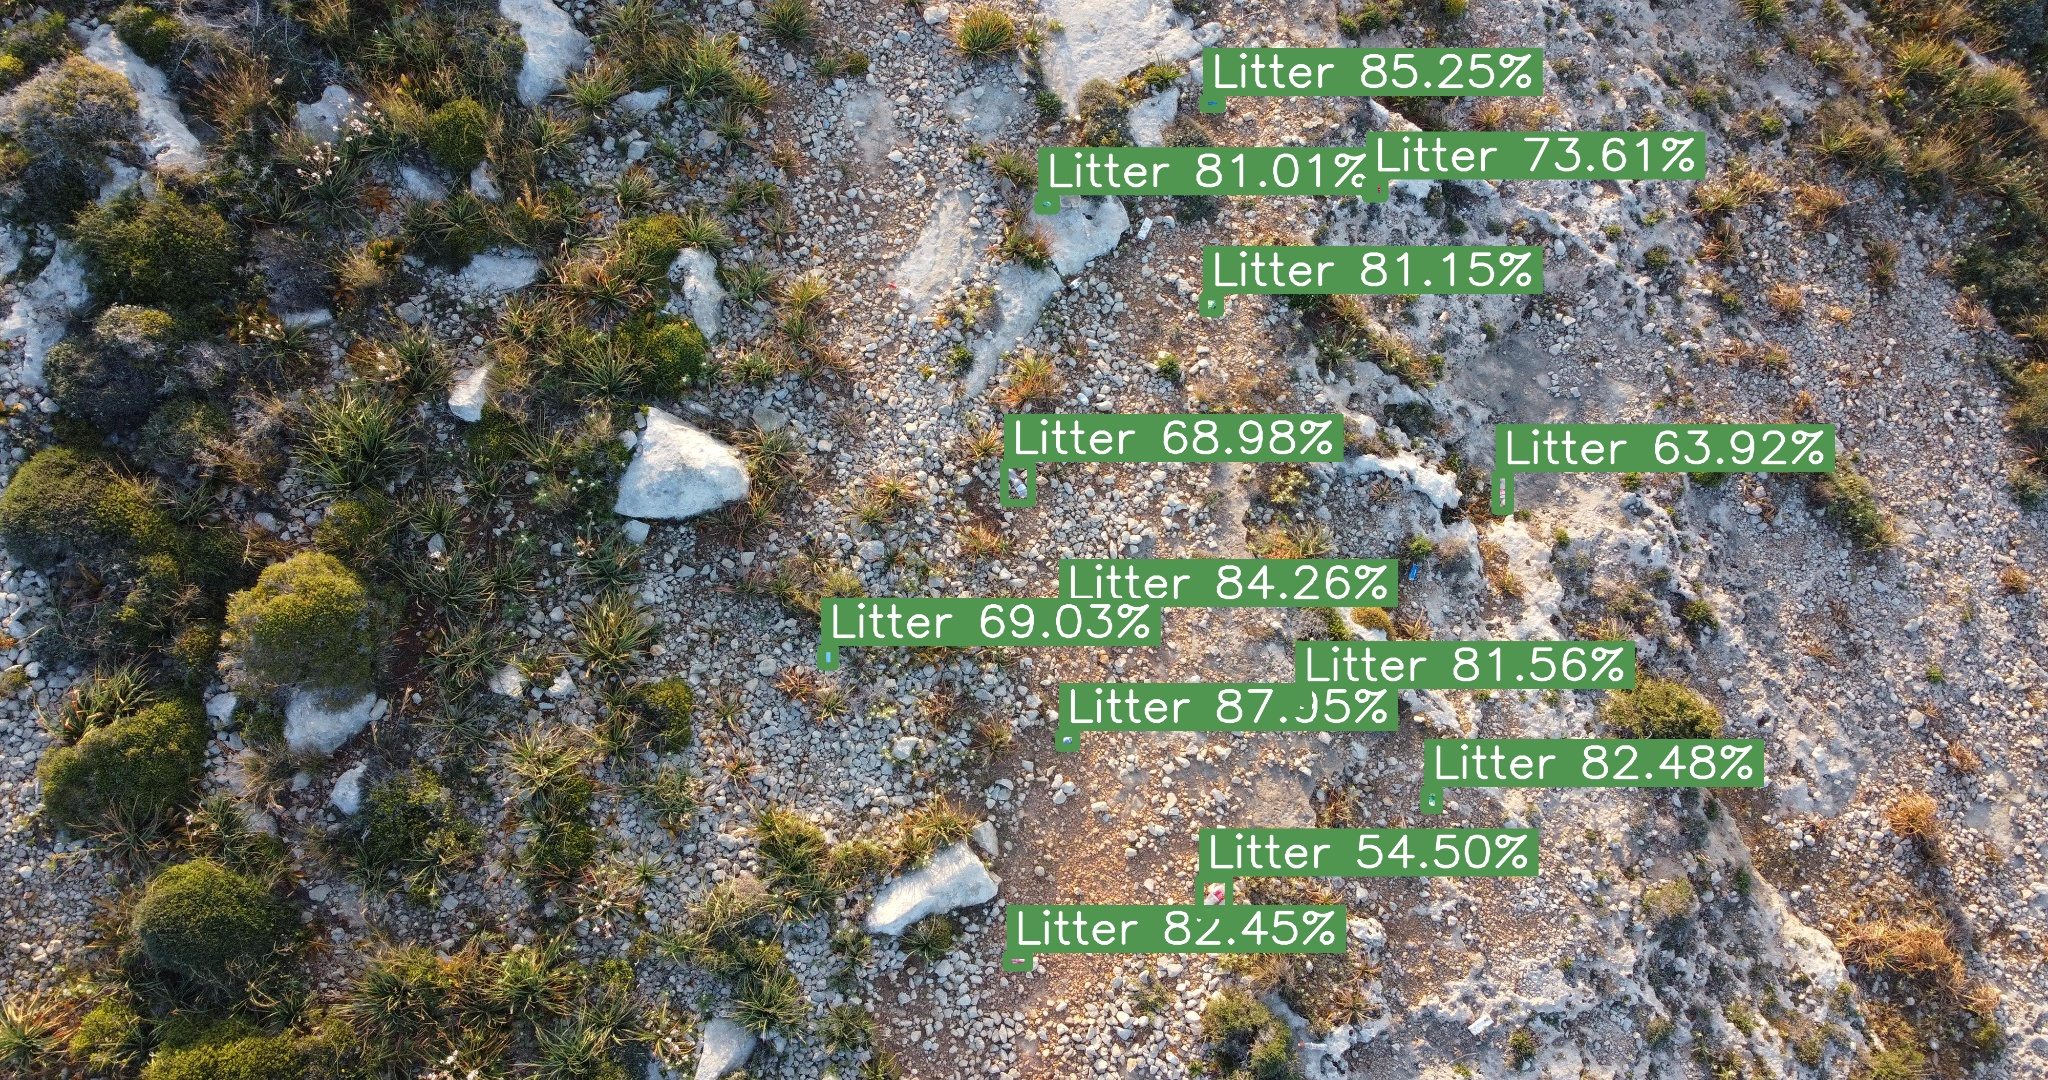
\includegraphics[width=0.47\textwidth]{visual3.jpg} &
    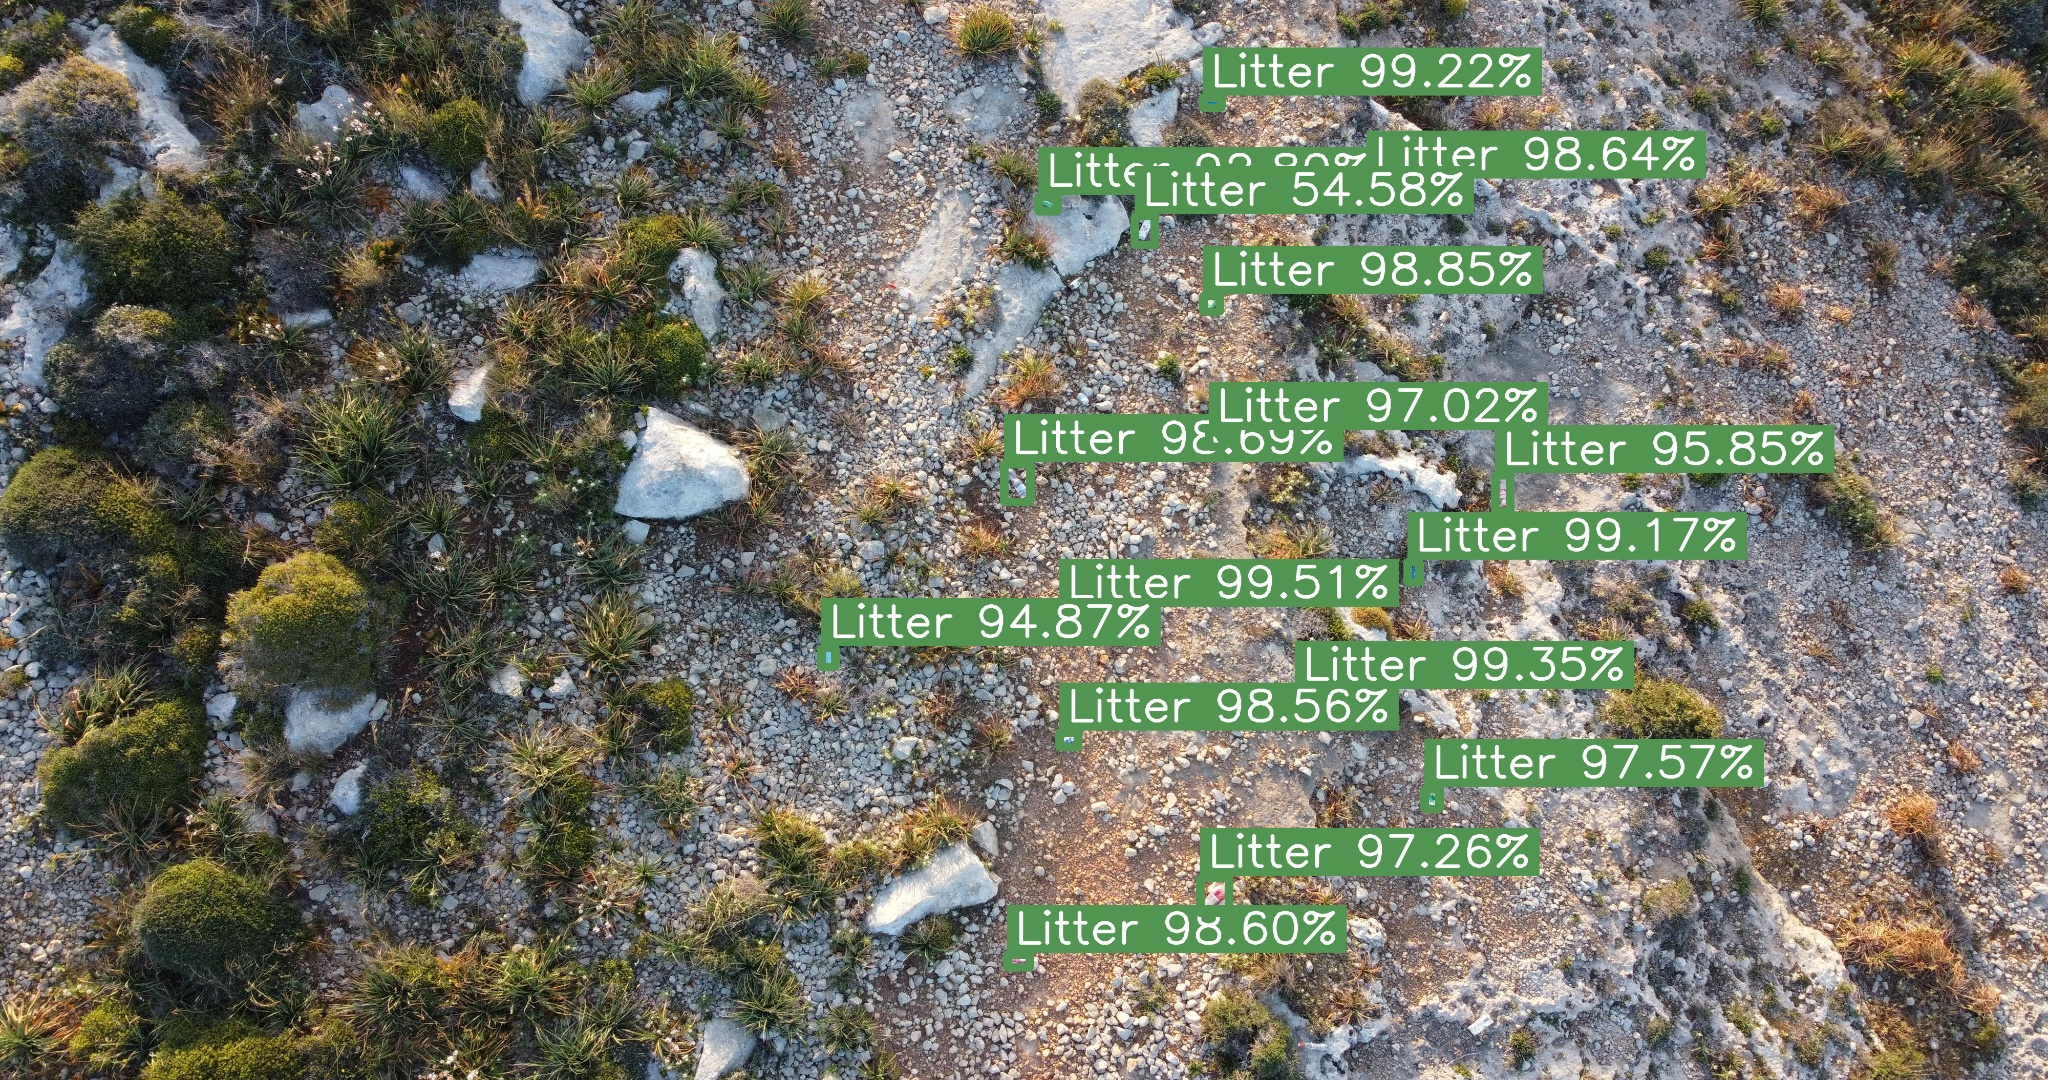
\includegraphics[width=0.47\textwidth]{visual4.jpg} \\
    \small (c) & \small (d) \\
  \end{tabular}
  \caption{Sample predictions on test subset images from detection models trained on the \gls{soda} dataset. Subfigures (a) and (c) show outputs from the baseline models, while (b) and (d) present predictions from their corresponding student models. Subfigures (a) and (b) illustrate RetinaNet results at an altitude of 1 metre; (c) and (d) show outputs from Faster \gls{rcnn}.}
  \label{fig:visuals_soda}
\end{figure}

Examining the visual results from the within-dataset experiments, as shown in Figure \ref{fig:visuals_soda}, it is evident that the integration of \gls{lupi} results in a noticeable improvement over the baseline model. In subfigures (a) and (b), this improvement is clear: although both RetinaNet models successfully detect all litter objects, the \gls{lupi} student model produces higher confidence scores, particularly in scenarios tailored for detection at a 1-metre altitude.
In subfigures (c) and (d), where detection becomes more challenging due to the significantly higher altitude, the improvement achieved by the Faster \gls{rcnn} student model is even more evident. It identifies more litter instances than the corresponding baseline and assigns higher confidence scores to its predictions. This further reinforces the practical value of incorporating the proposed approach.

In the cross-dataset evaluation, where models trained on the \gls{soda} dataset were tested on other binary litter detection datasets to assess how well the proposed approach generalises, the improvement is also clearly visible. This is illustrated in Figures \ref{fig:visuals_bdw} and \ref{fig:visuals_uavvaste}.

\begin{figure}[ht]
  \centering
  \begin{tabular}{cc}
    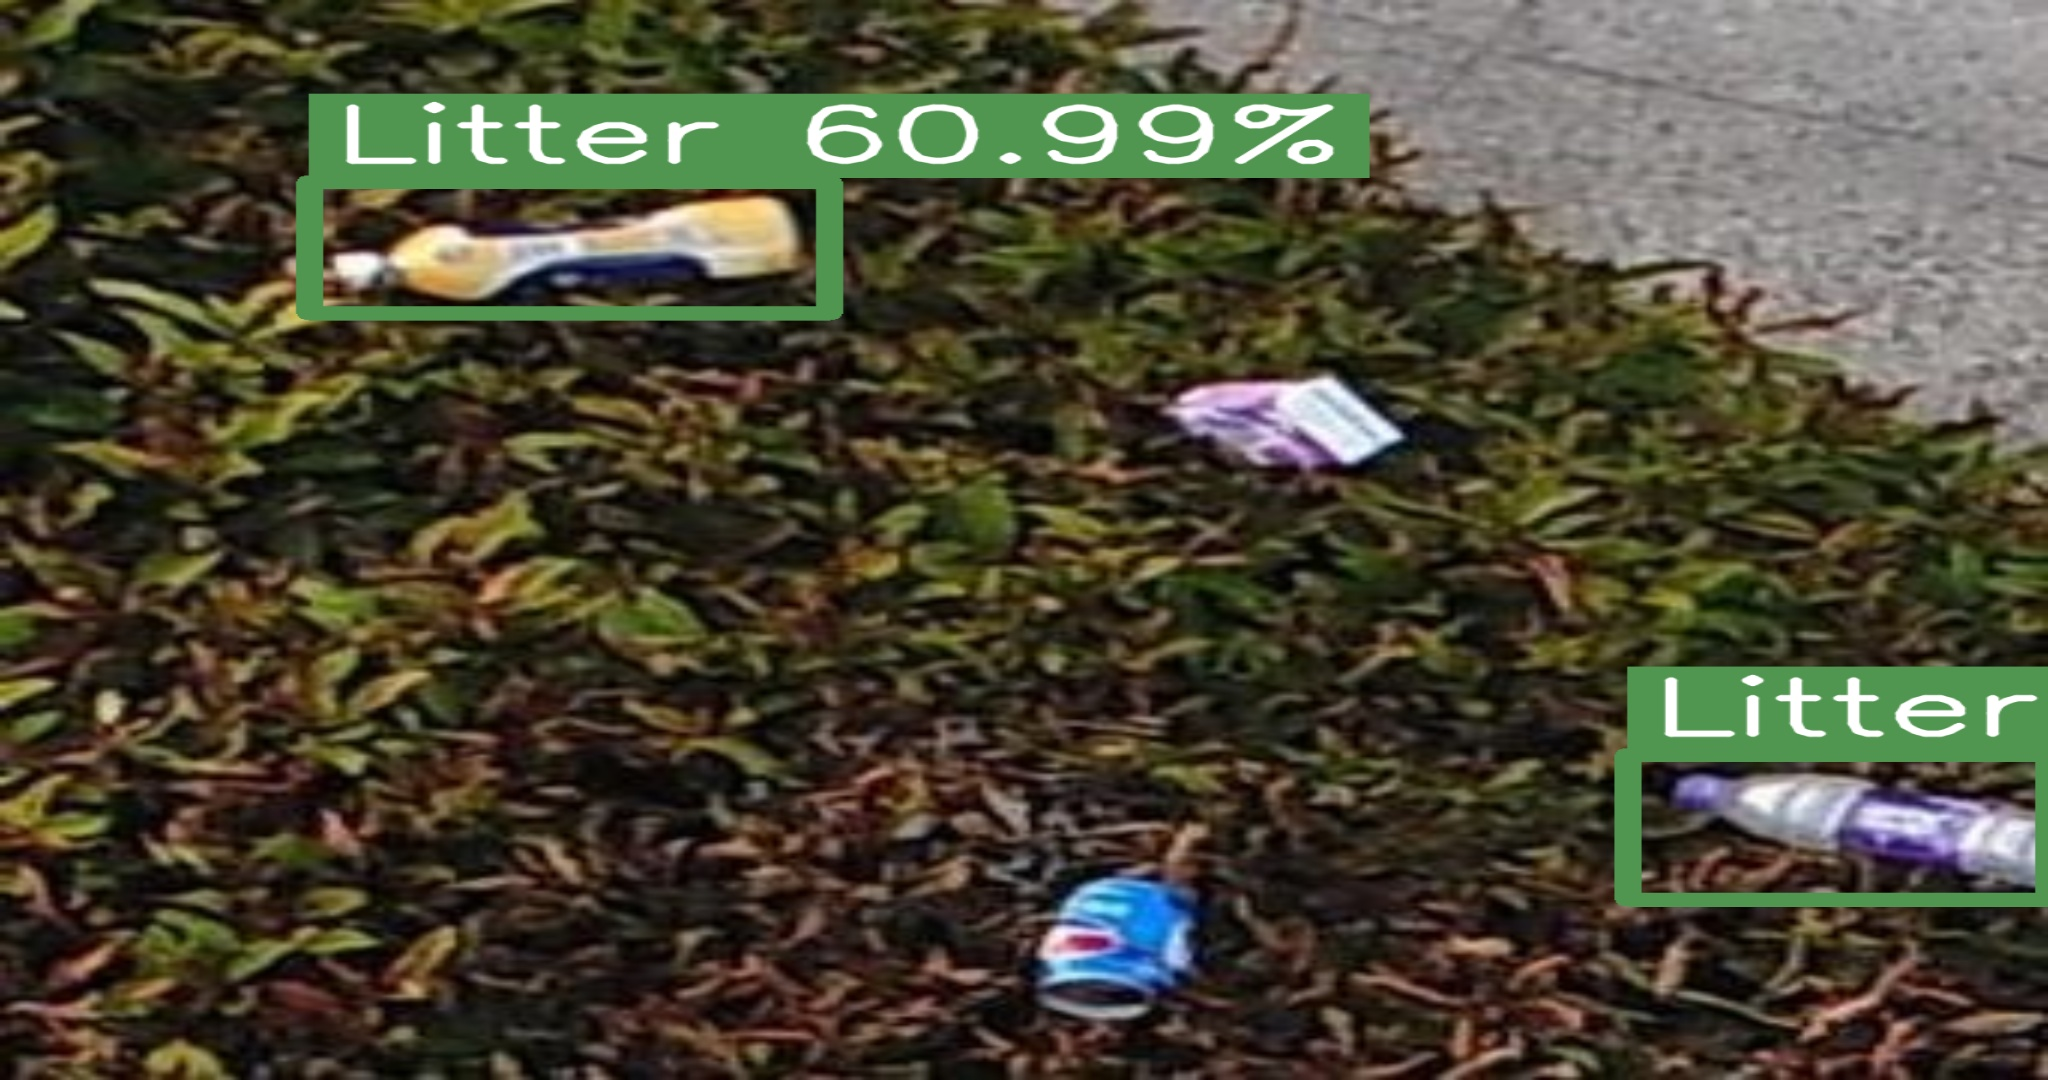
\includegraphics[width=0.47\textwidth]{visual9.jpg} &
    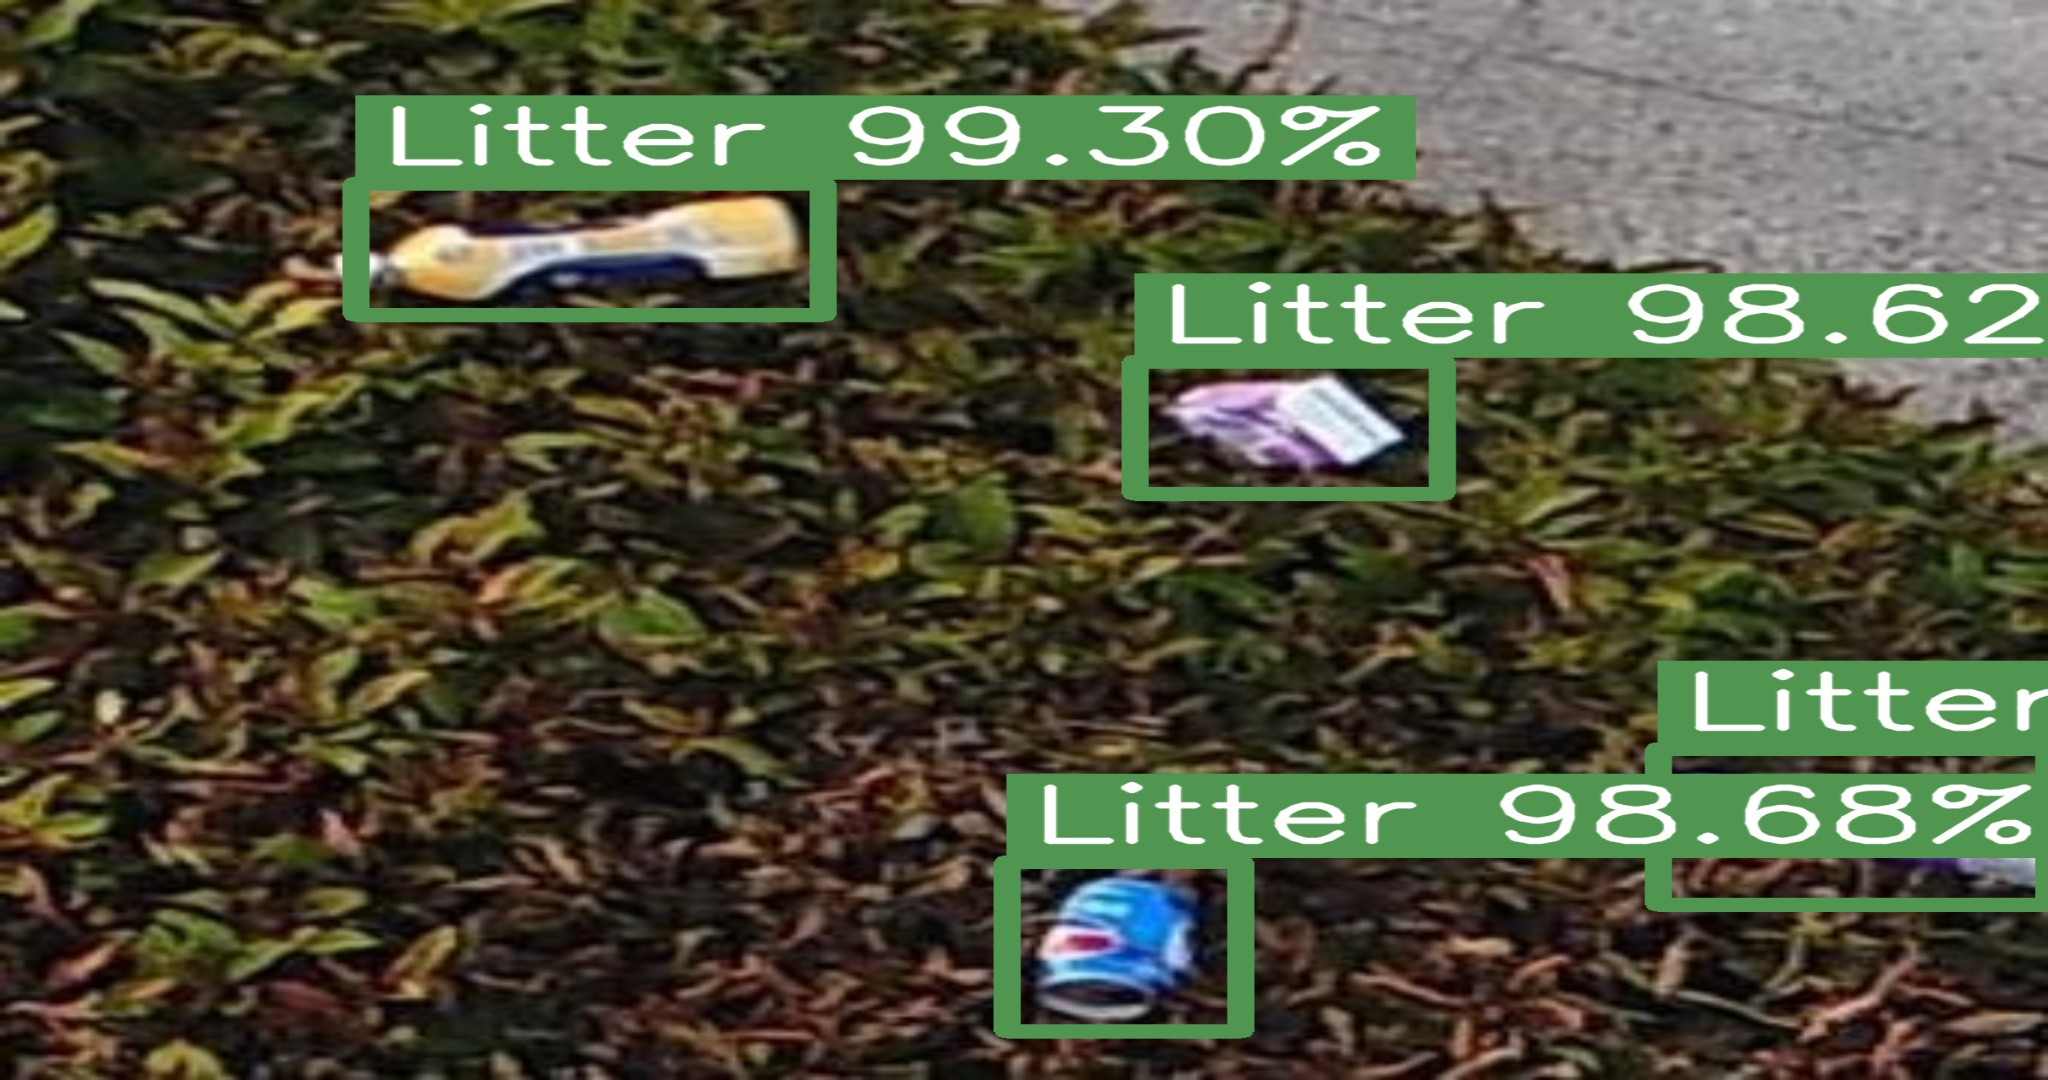
\includegraphics[width=0.47\textwidth]{visual10.jpg} \\
    \small (a) & \small (b) \\
  \end{tabular}
  \caption{Sample predictions on test subset images from the \gls{fcos} detection model, trained on the \gls{soda} dataset and evaluated on the \gls{bdw} dataset. Subfigure (a) shows outputs from the baseline model, while (b) presents predictions from the corresponding student model.}
  \label{fig:visuals_bdw}
\end{figure}

\begin{figure}[ht]
  \centering
  \begin{tabular}{cc}
    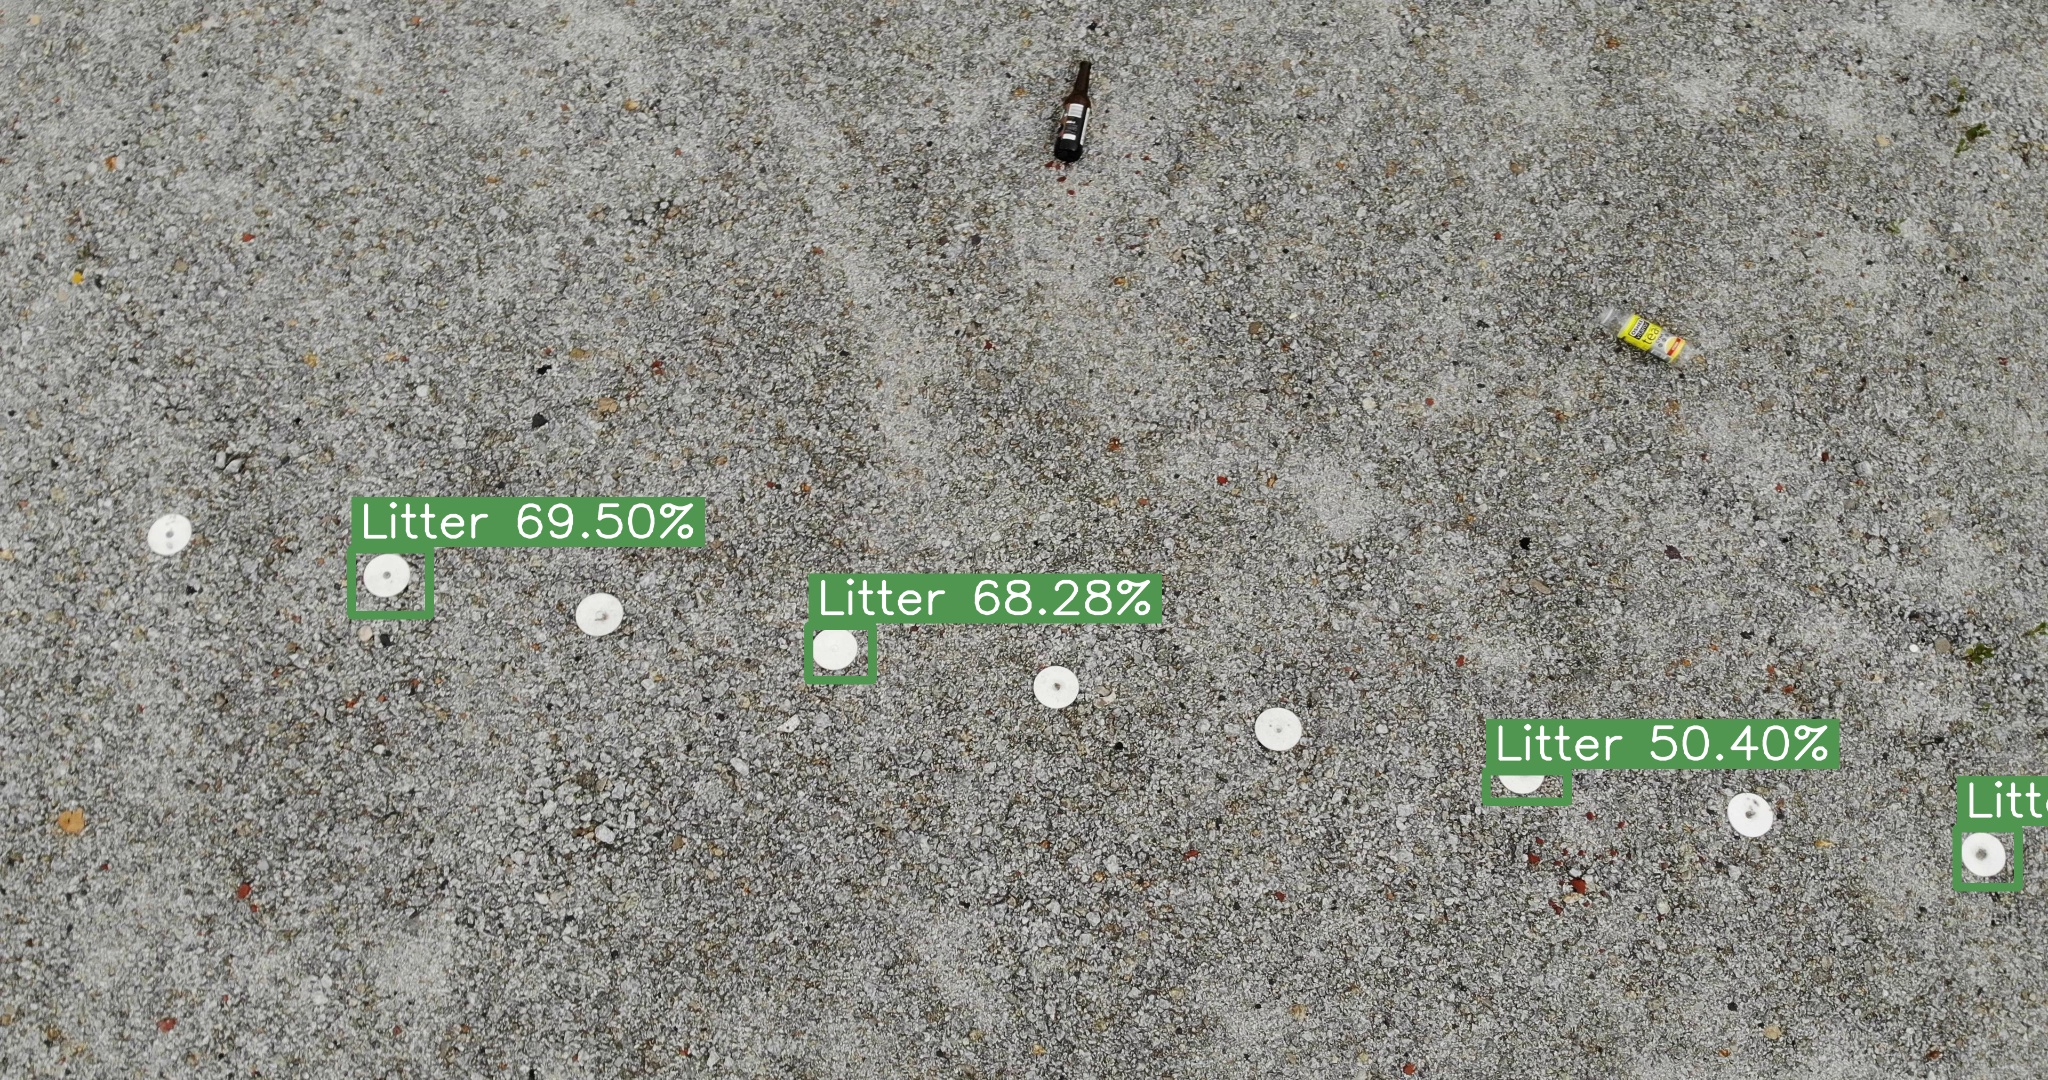
\includegraphics[width=0.47\textwidth]{visual11.jpg} &
    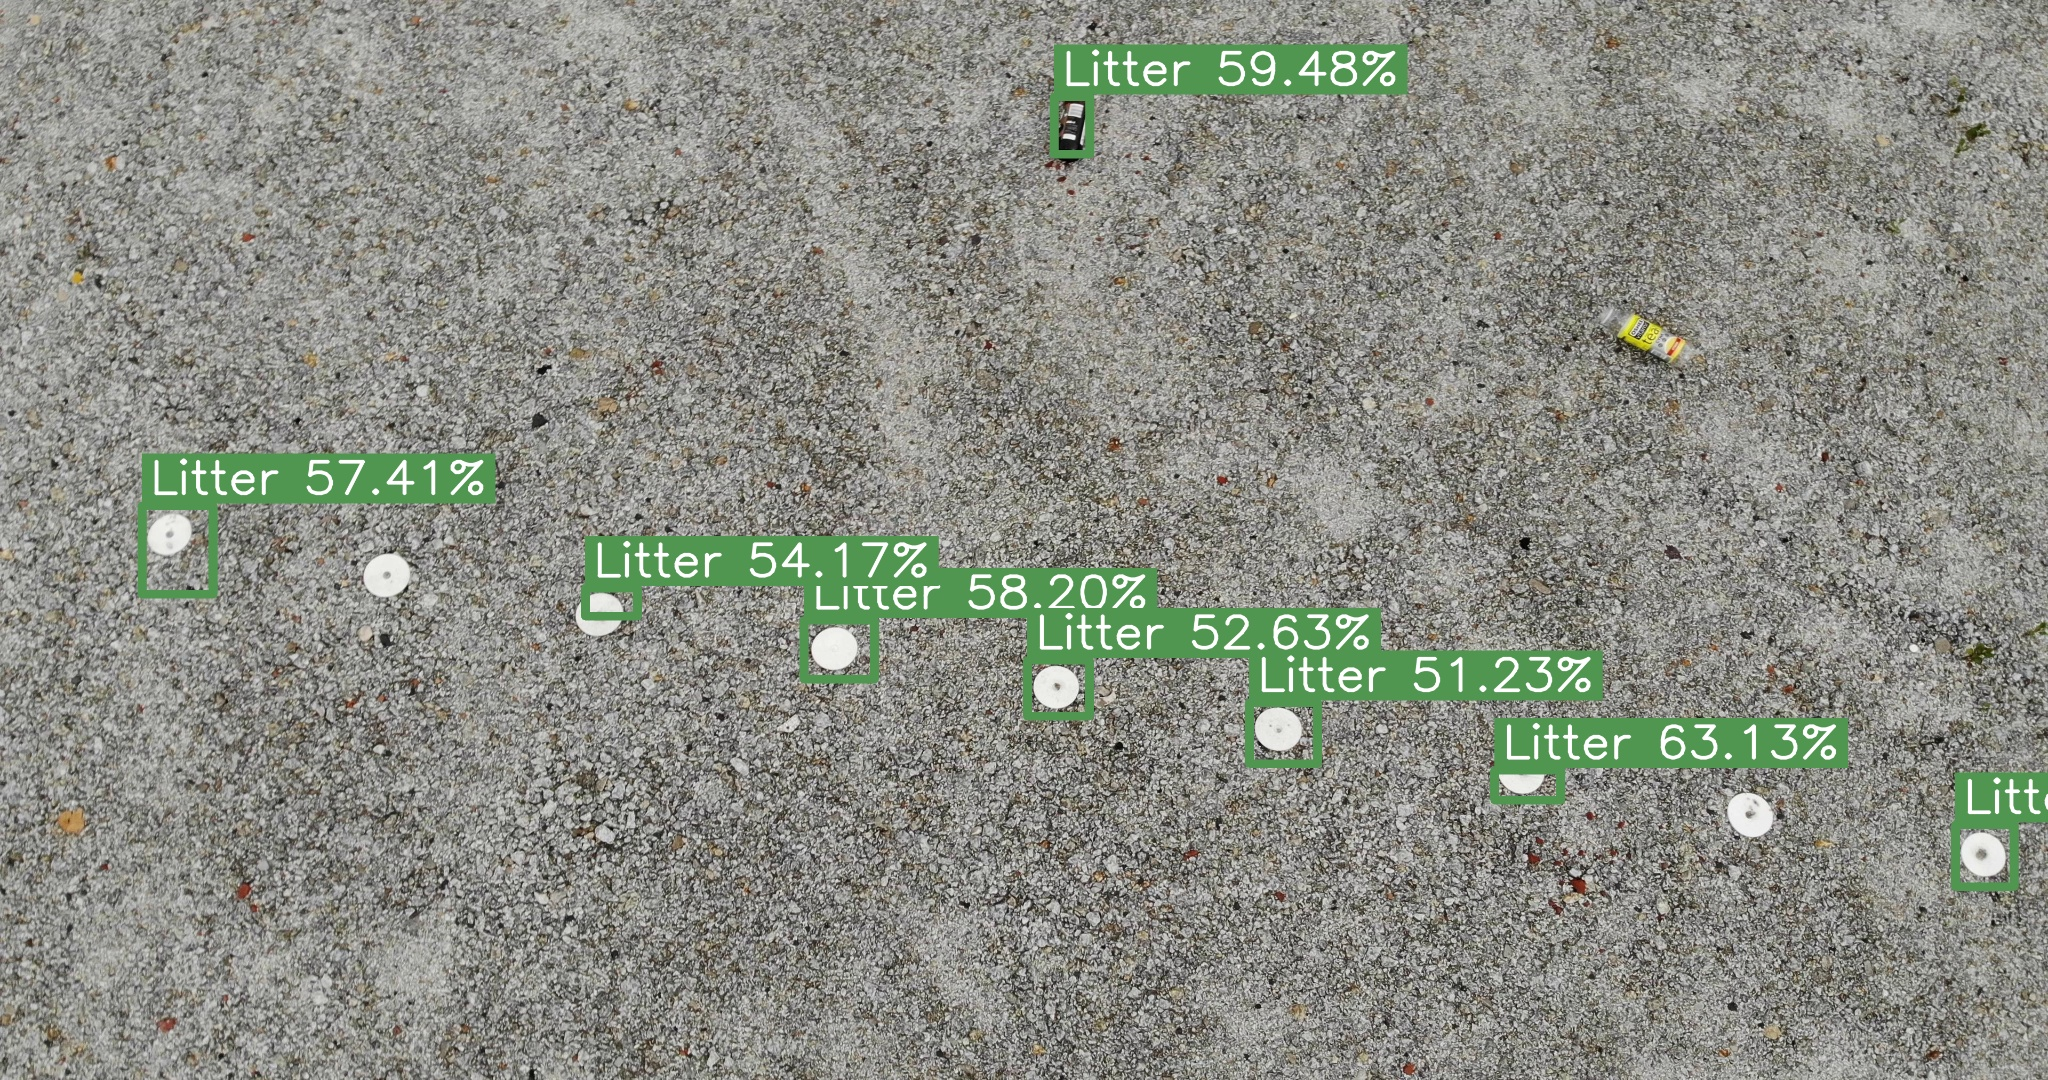
\includegraphics[width=0.47\textwidth]{visual12.jpg} \\
    \small (a) & \small (b) \\
  \end{tabular}
  \caption{Sample predictions on test subset images from the best-performing detection model, Faster \gls{rcnn}, trained on the \gls{soda} dataset and evaluated on the UAVVaste dataset. Subfigure (a) shows outputs from the baseline model, while (b) presents predictions from the corresponding student model.}
  \label{fig:visuals_uavvaste}
\end{figure}

For the \gls{bdw} dataset, using the best-performing model based on the \gls{fcos} architecture, the student model detected more litter instances than the baseline. Similarly, for UAVVaste, where the top-performing model was Faster \gls{rcnn}, the student model again identified more objects. In both cases, the continued trend of higher confidence scores reinforces the notion that integrating \gls{lupi} contributes to more effective and robust learning.

A similar trend is evident in the general object detection task with multi-label detection, as demonstrated in the Pascal \gls{voc} 2012 experiment. The improvement is particularly noticeable when using the best-performing architecture, Faster \gls{rcnn}, as shown in Figure \ref{fig:visuals_pascal_voc}.

\begin{figure}[ht]
  \centering
  \begin{tabular}{cc}
    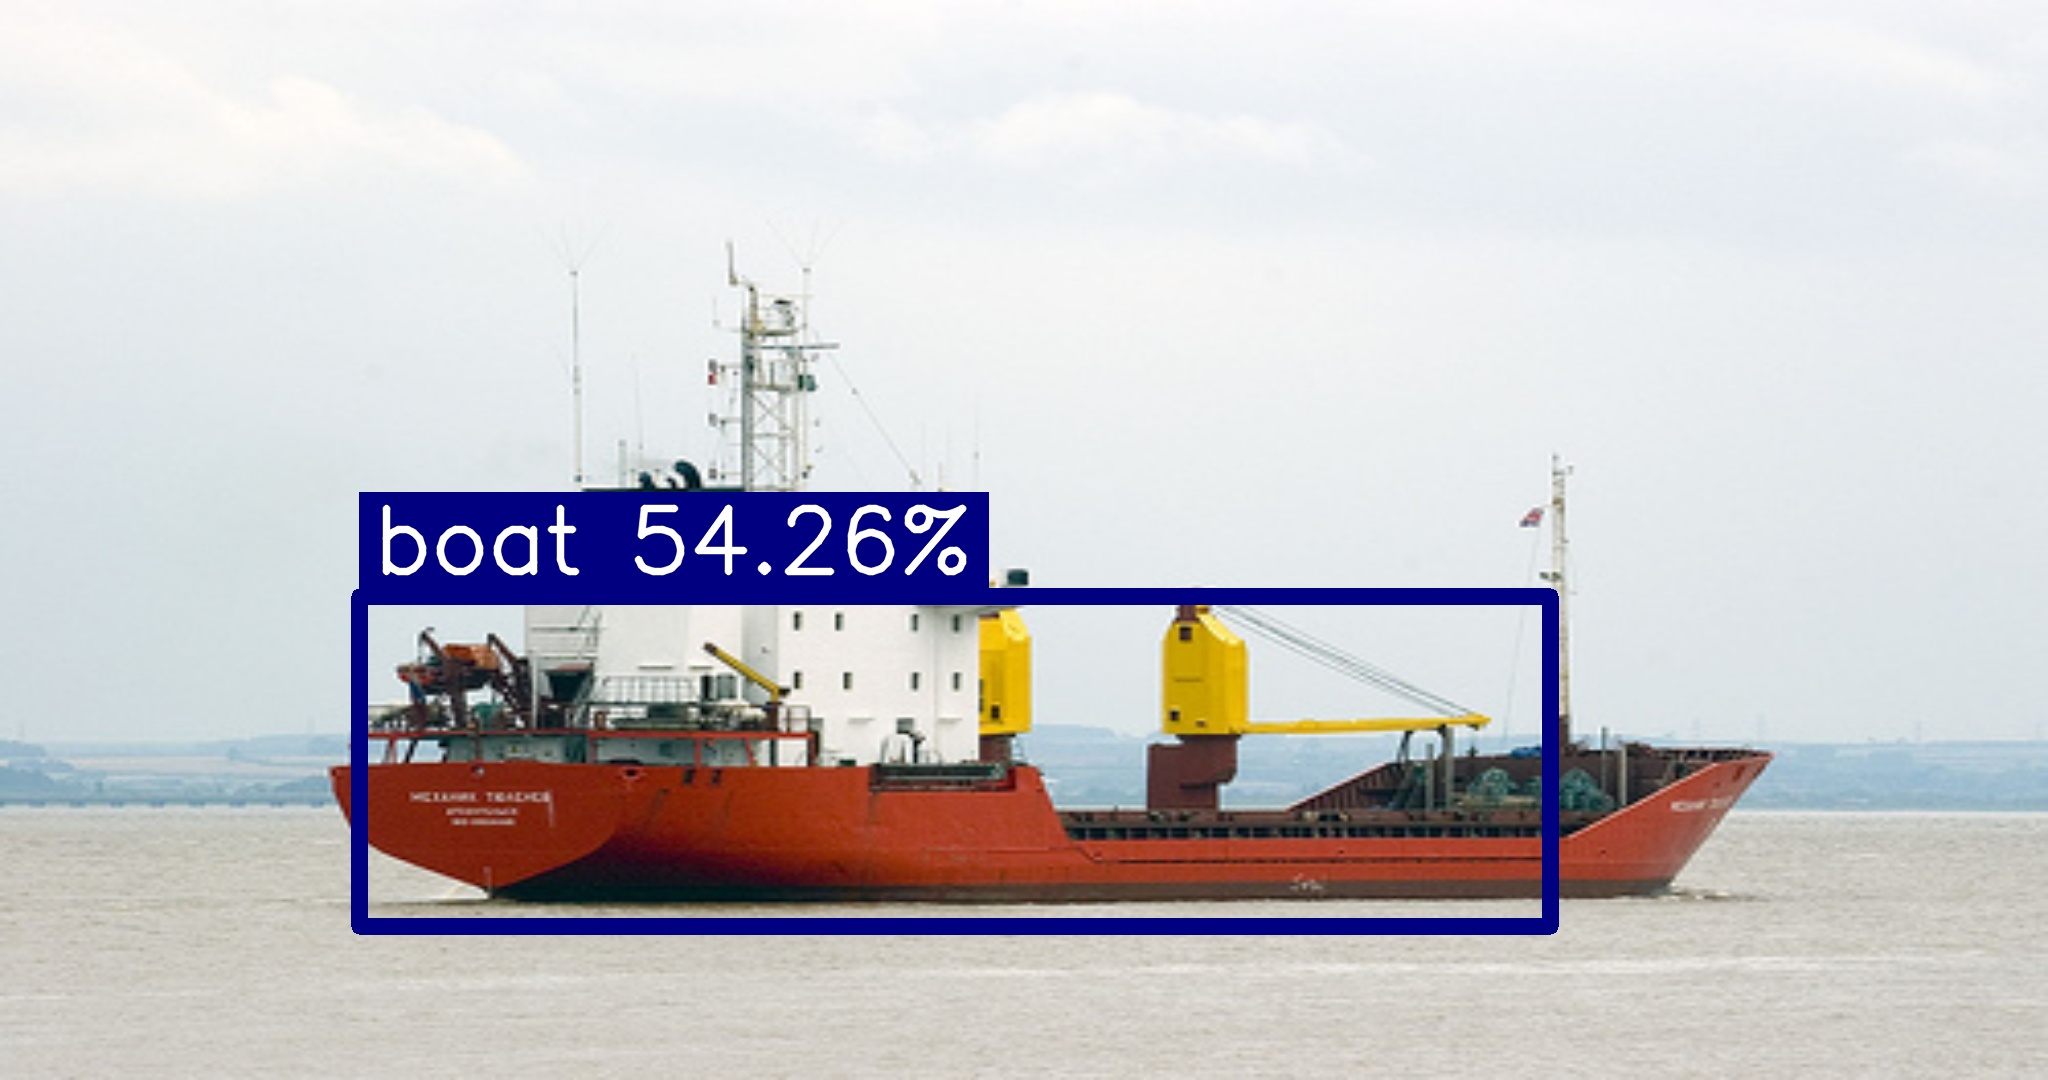
\includegraphics[width=0.47\textwidth]{visual5.jpg} &
    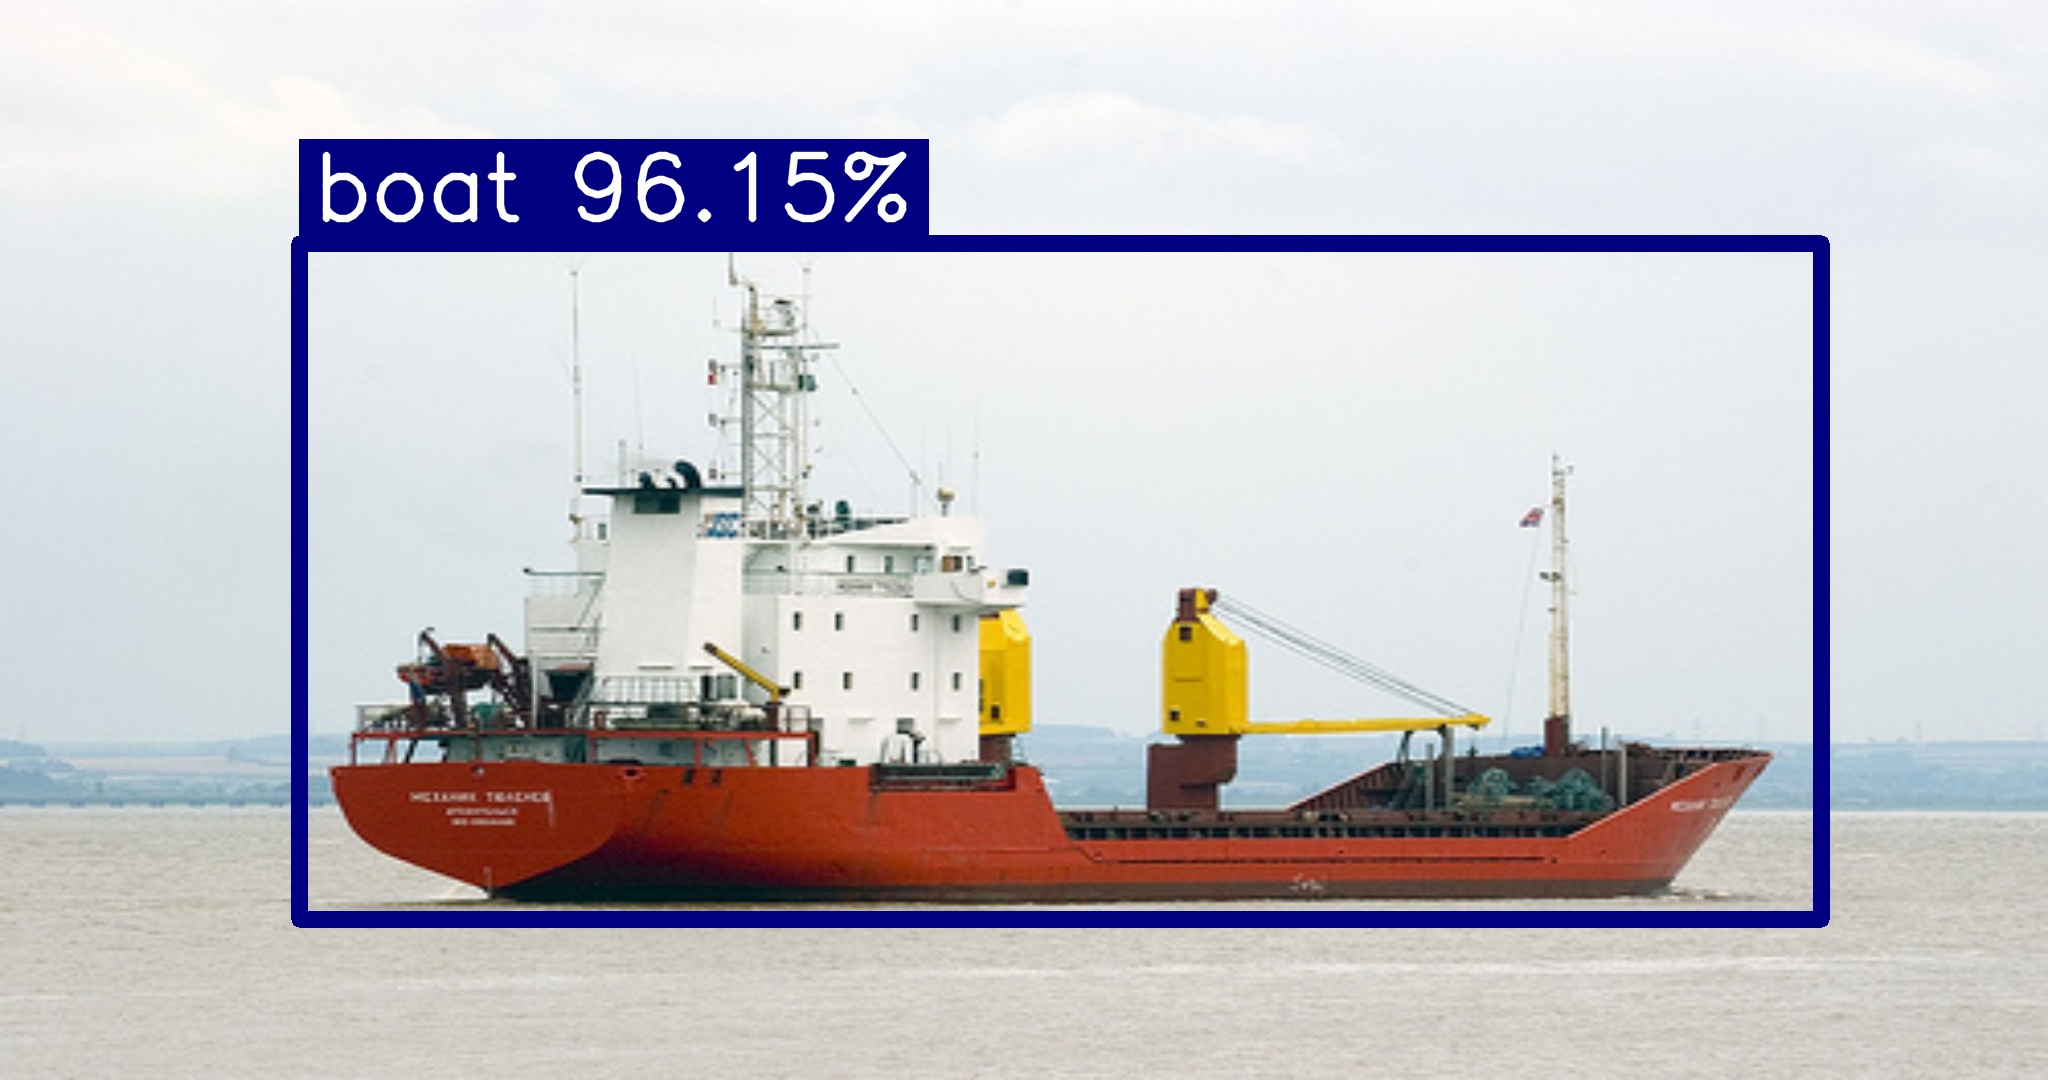
\includegraphics[width=0.47\textwidth]{visual6.jpg} \\
    \small (a) & \small (b) \\
    \addlinespace[1em]
    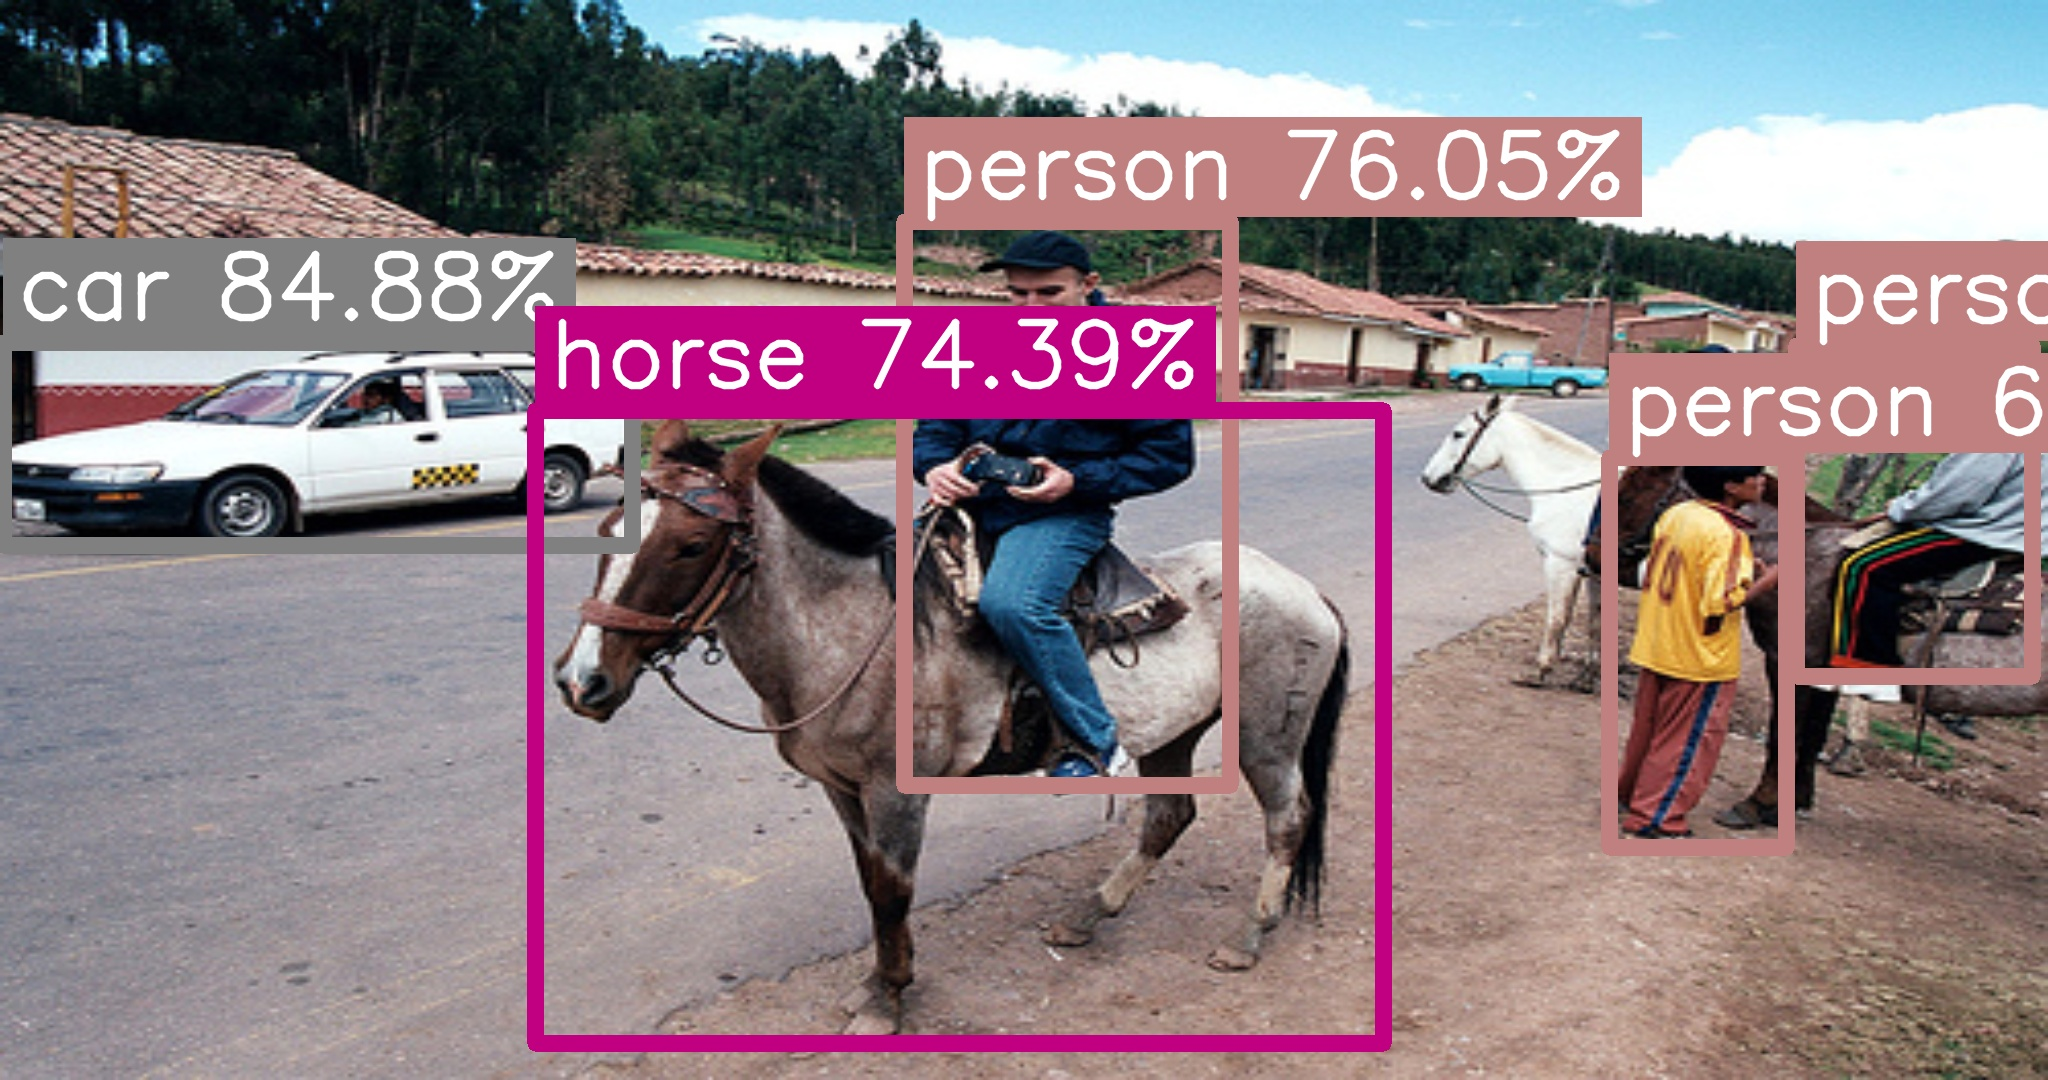
\includegraphics[width=0.47\textwidth]{visual7.jpg} &
    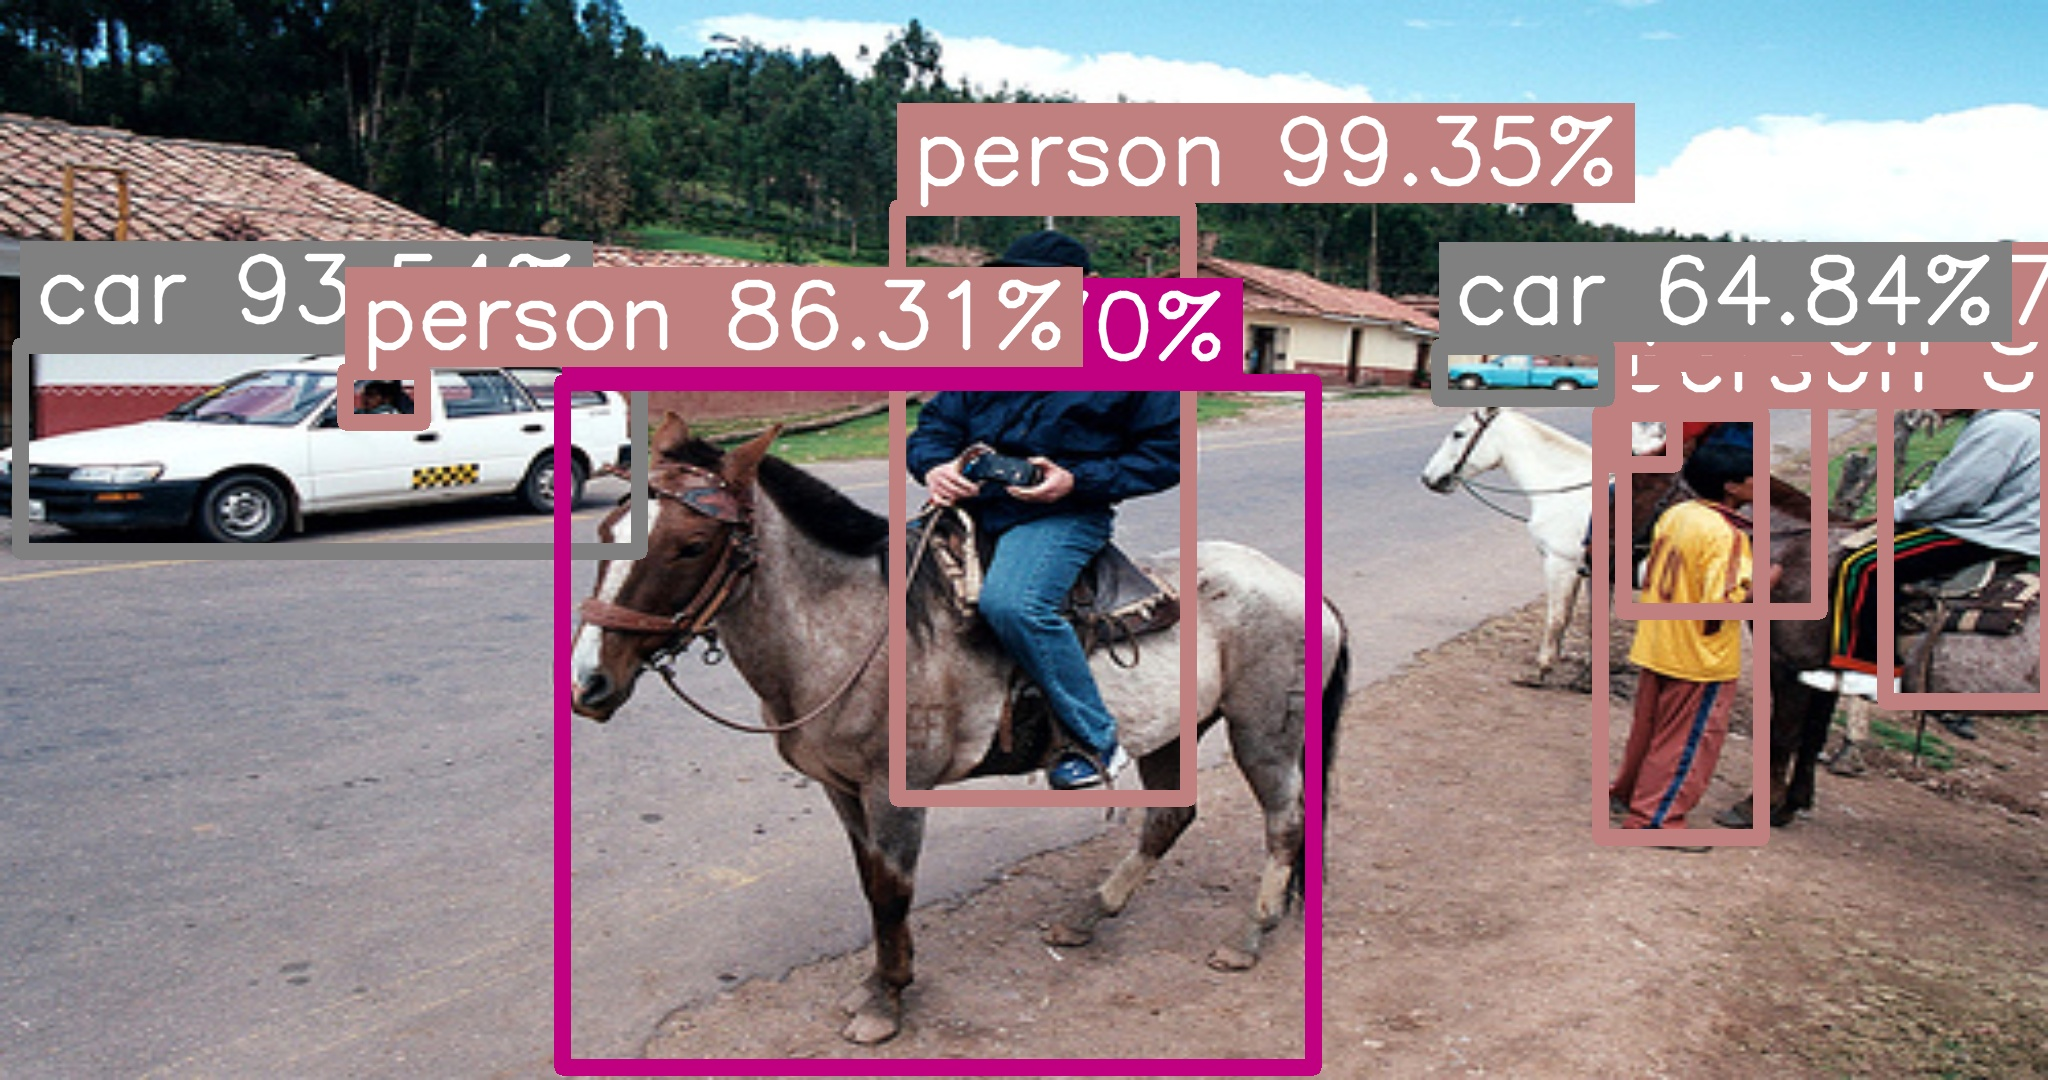
\includegraphics[width=0.47\textwidth]{visual8.jpg} \\
    \small (c) & \small (d) \\
  \end{tabular}
  \caption{Sample predictions from the best-performing detection model, Faster \gls{rcnn}, trained on the Pascal \gls{voc} 2012 dataset. Subfigures (a) and (c) show outputs from the baseline model, while (b) and (d) present predictions from the corresponding student model.}
  \label{fig:visuals_pascal_voc}
\end{figure}

In the first example, the baseline prediction in (a) has a low detection score, and the bounding box does not fully capture the object of interest. In contrast, the student model produces a bounding box that accurately encloses the object, reflecting a more precise prediction. In the second example, the baseline prediction in (c) performs reasonably well but misses some important elements. It fails to detect the person inside the car and overlooks the car in the background, while also assigning relatively low confidence scores, which negatively impact the \gls{map}.
In comparison, the student prediction in (d) correctly identifies all the relevant objects except for the horse in the background. This improvement in both object coverage and confidence underscores the overall efficacy of the proposed methodology, demonstrating its advantages in both litter detection and general object detection tasks.


\section{Visual Interpretability of Model Predictions}
\label{sec:5_interpretability}

Additional tests were conducted to evaluate the visual interpretability of how the models make predictions on specific images. To facilitate this, three commonly used class activation mapping techniques were employed to assess any improvements between the baseline and student models from a feature-based perspective. These methods included Grad-\gls{cam} \cite{gradcam}, Grad-\gls{cam}++ \cite{gradcam_plus_plus}, and Eigen-\gls{cam} \cite{eigencam}.

Grad-\gls{cam} and Grad-\gls{cam}++ both use a gradient-based approach, where the gradient of a target concept is propagated to the final convolutional layer, resulting in a coarse localisation map that highlights key regions in the image relevant for the prediction. Grad-\gls{cam}++ enhances this process by providing clearer visual explanations, improving object localisation and enabling better interpretation of multiple object instances within a single image. Meanwhile, Eigen-\gls{cam} utilises principal components derived from the learned features in the convolutional layers, offering a different approach to explaining model predictions. 


This test was carried out across all selected architecture types, using the specific target layer where the distillation process took place for each model (see Subsection \ref{subsec:4_student}) to examine whether there were visual differences in feature-based learning between the baseline and student models. Although this analysis was conducted on all trained models and across various images for consistency, only the results from models trained on the \gls{soda} 1-metre altitude dataset are presented here for brevity. This decision was made as the experiment yielded the most significant improvements under the proposed \gls{lupi}-based approach. The visual outcomes of this test are shown in Figure \ref{fig:gradcam_comparison}.

\begin{figure}[!ht]
    \centering
    \begin{tabular}{c}
        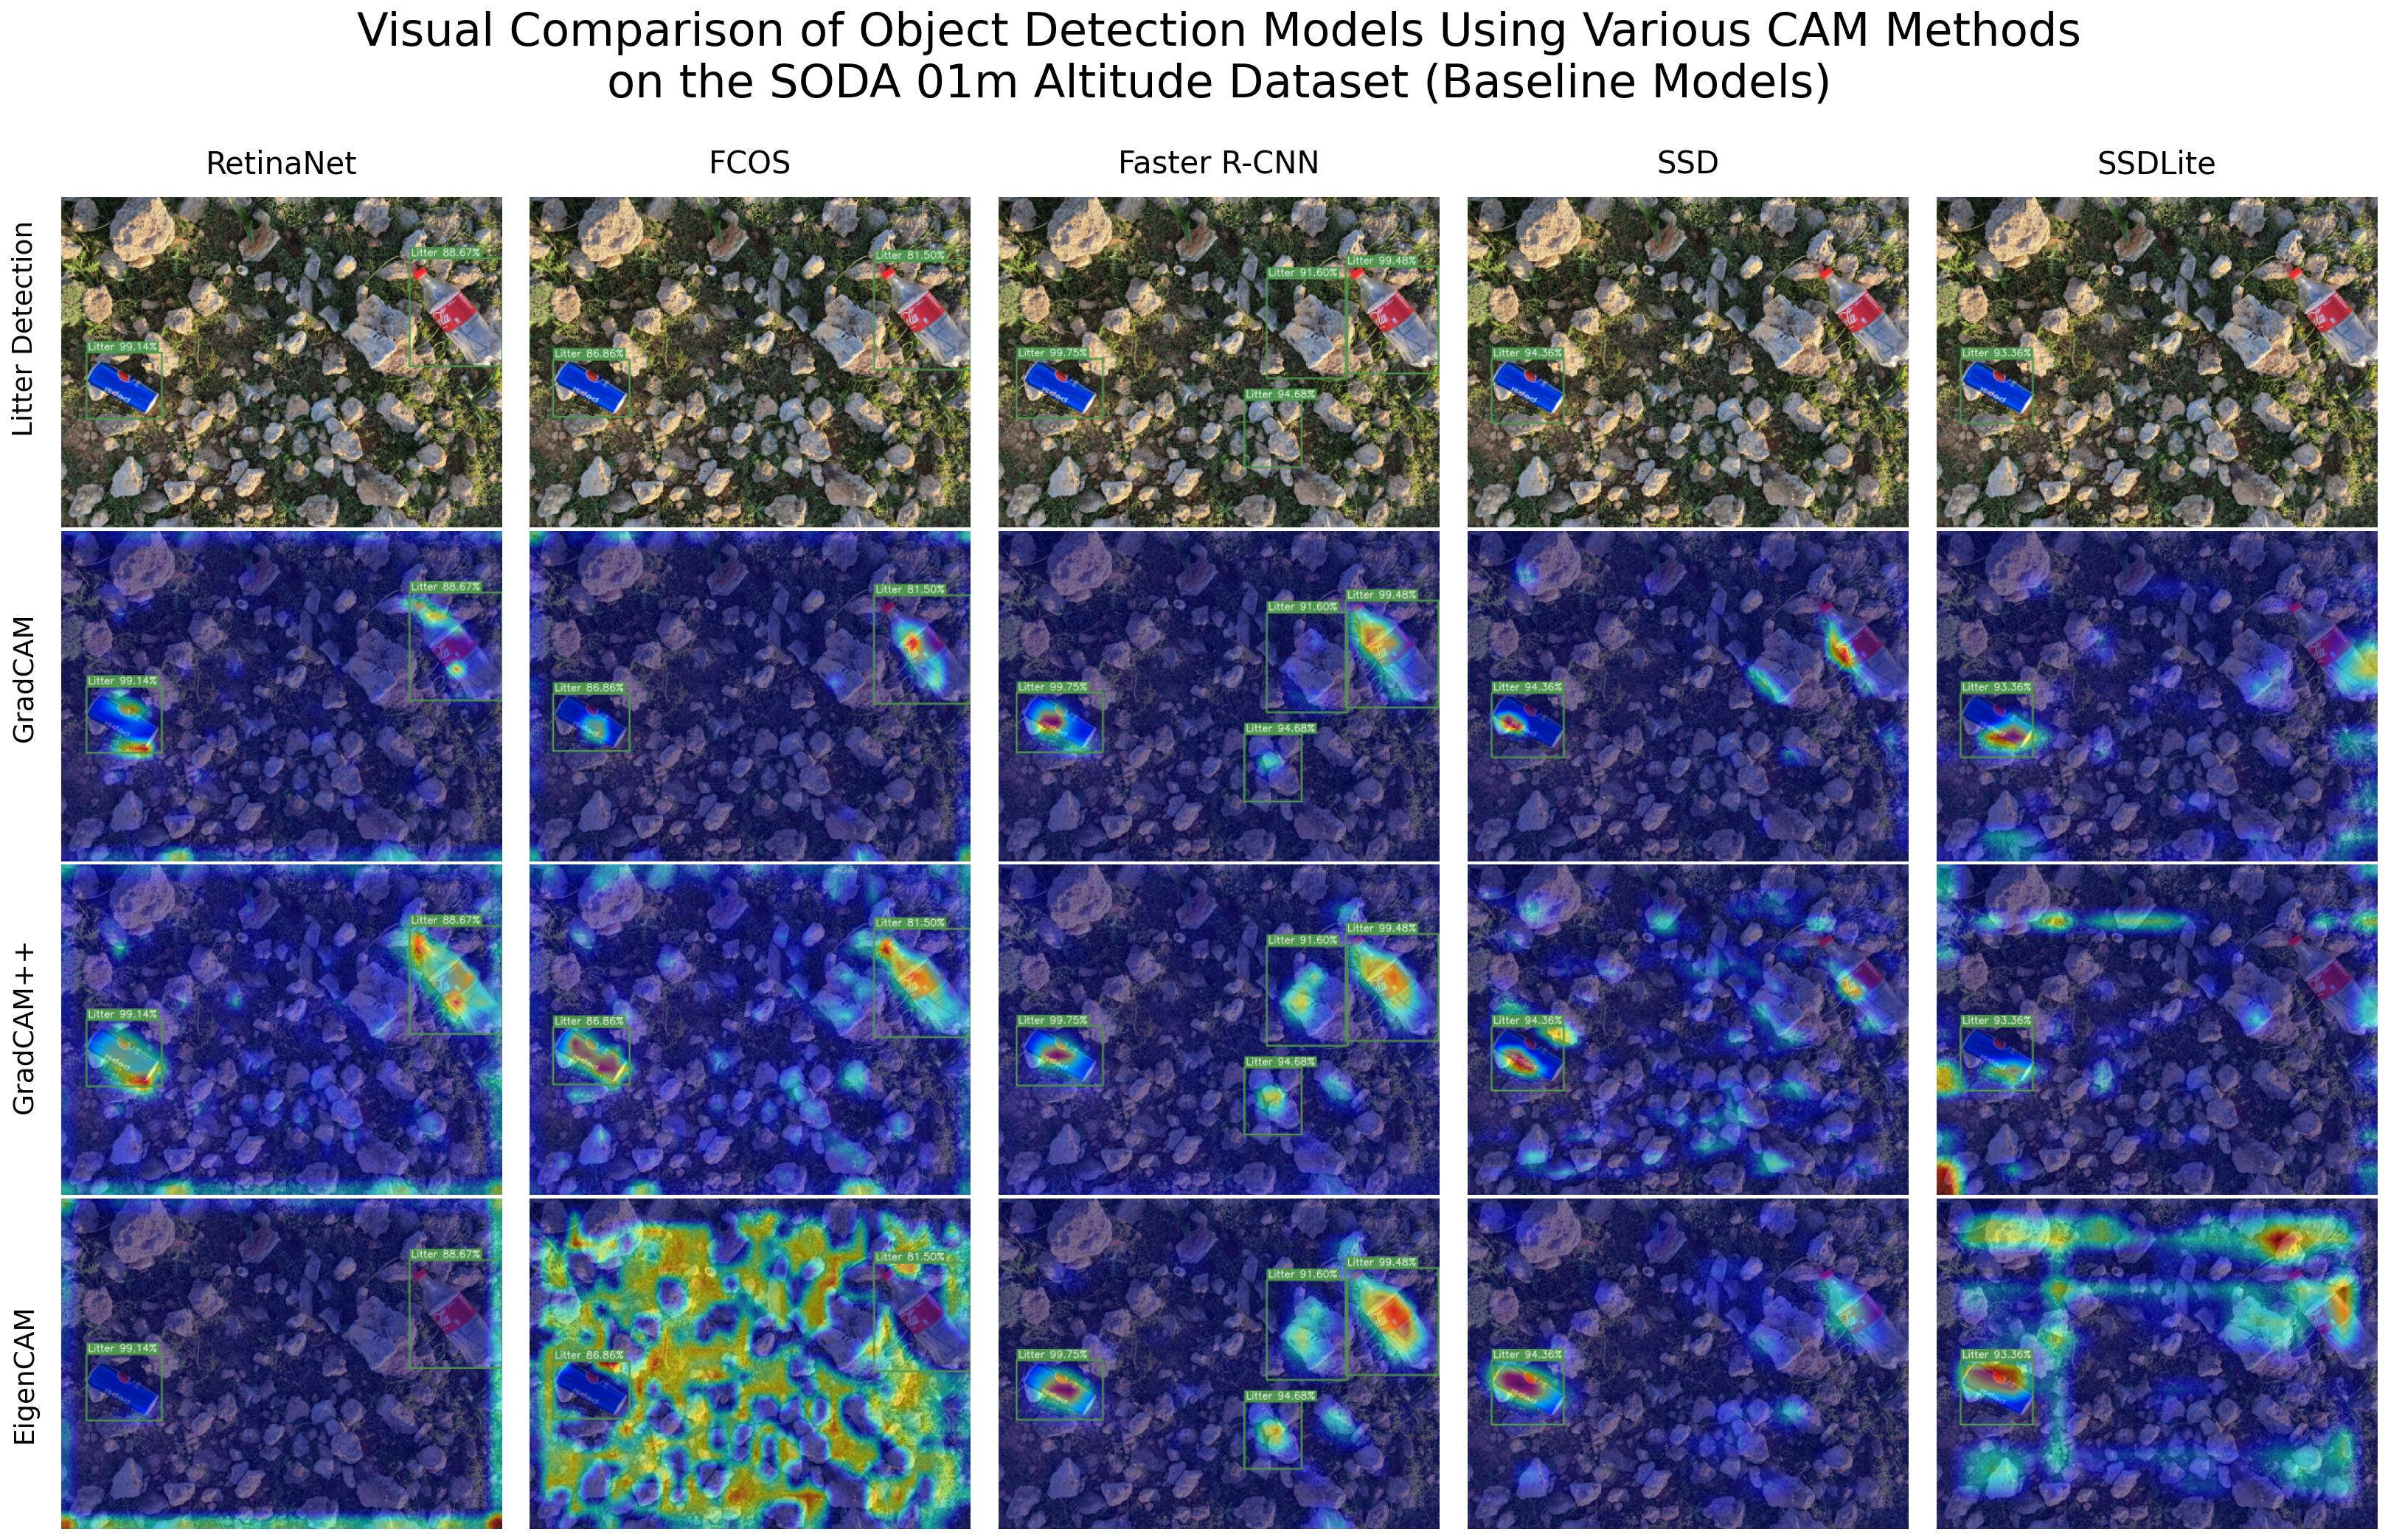
\includegraphics[width=0.9\textwidth]{gradcam_comparison_baseline.jpg} \\
        \small (a) \\
        \addlinespace[1em]
        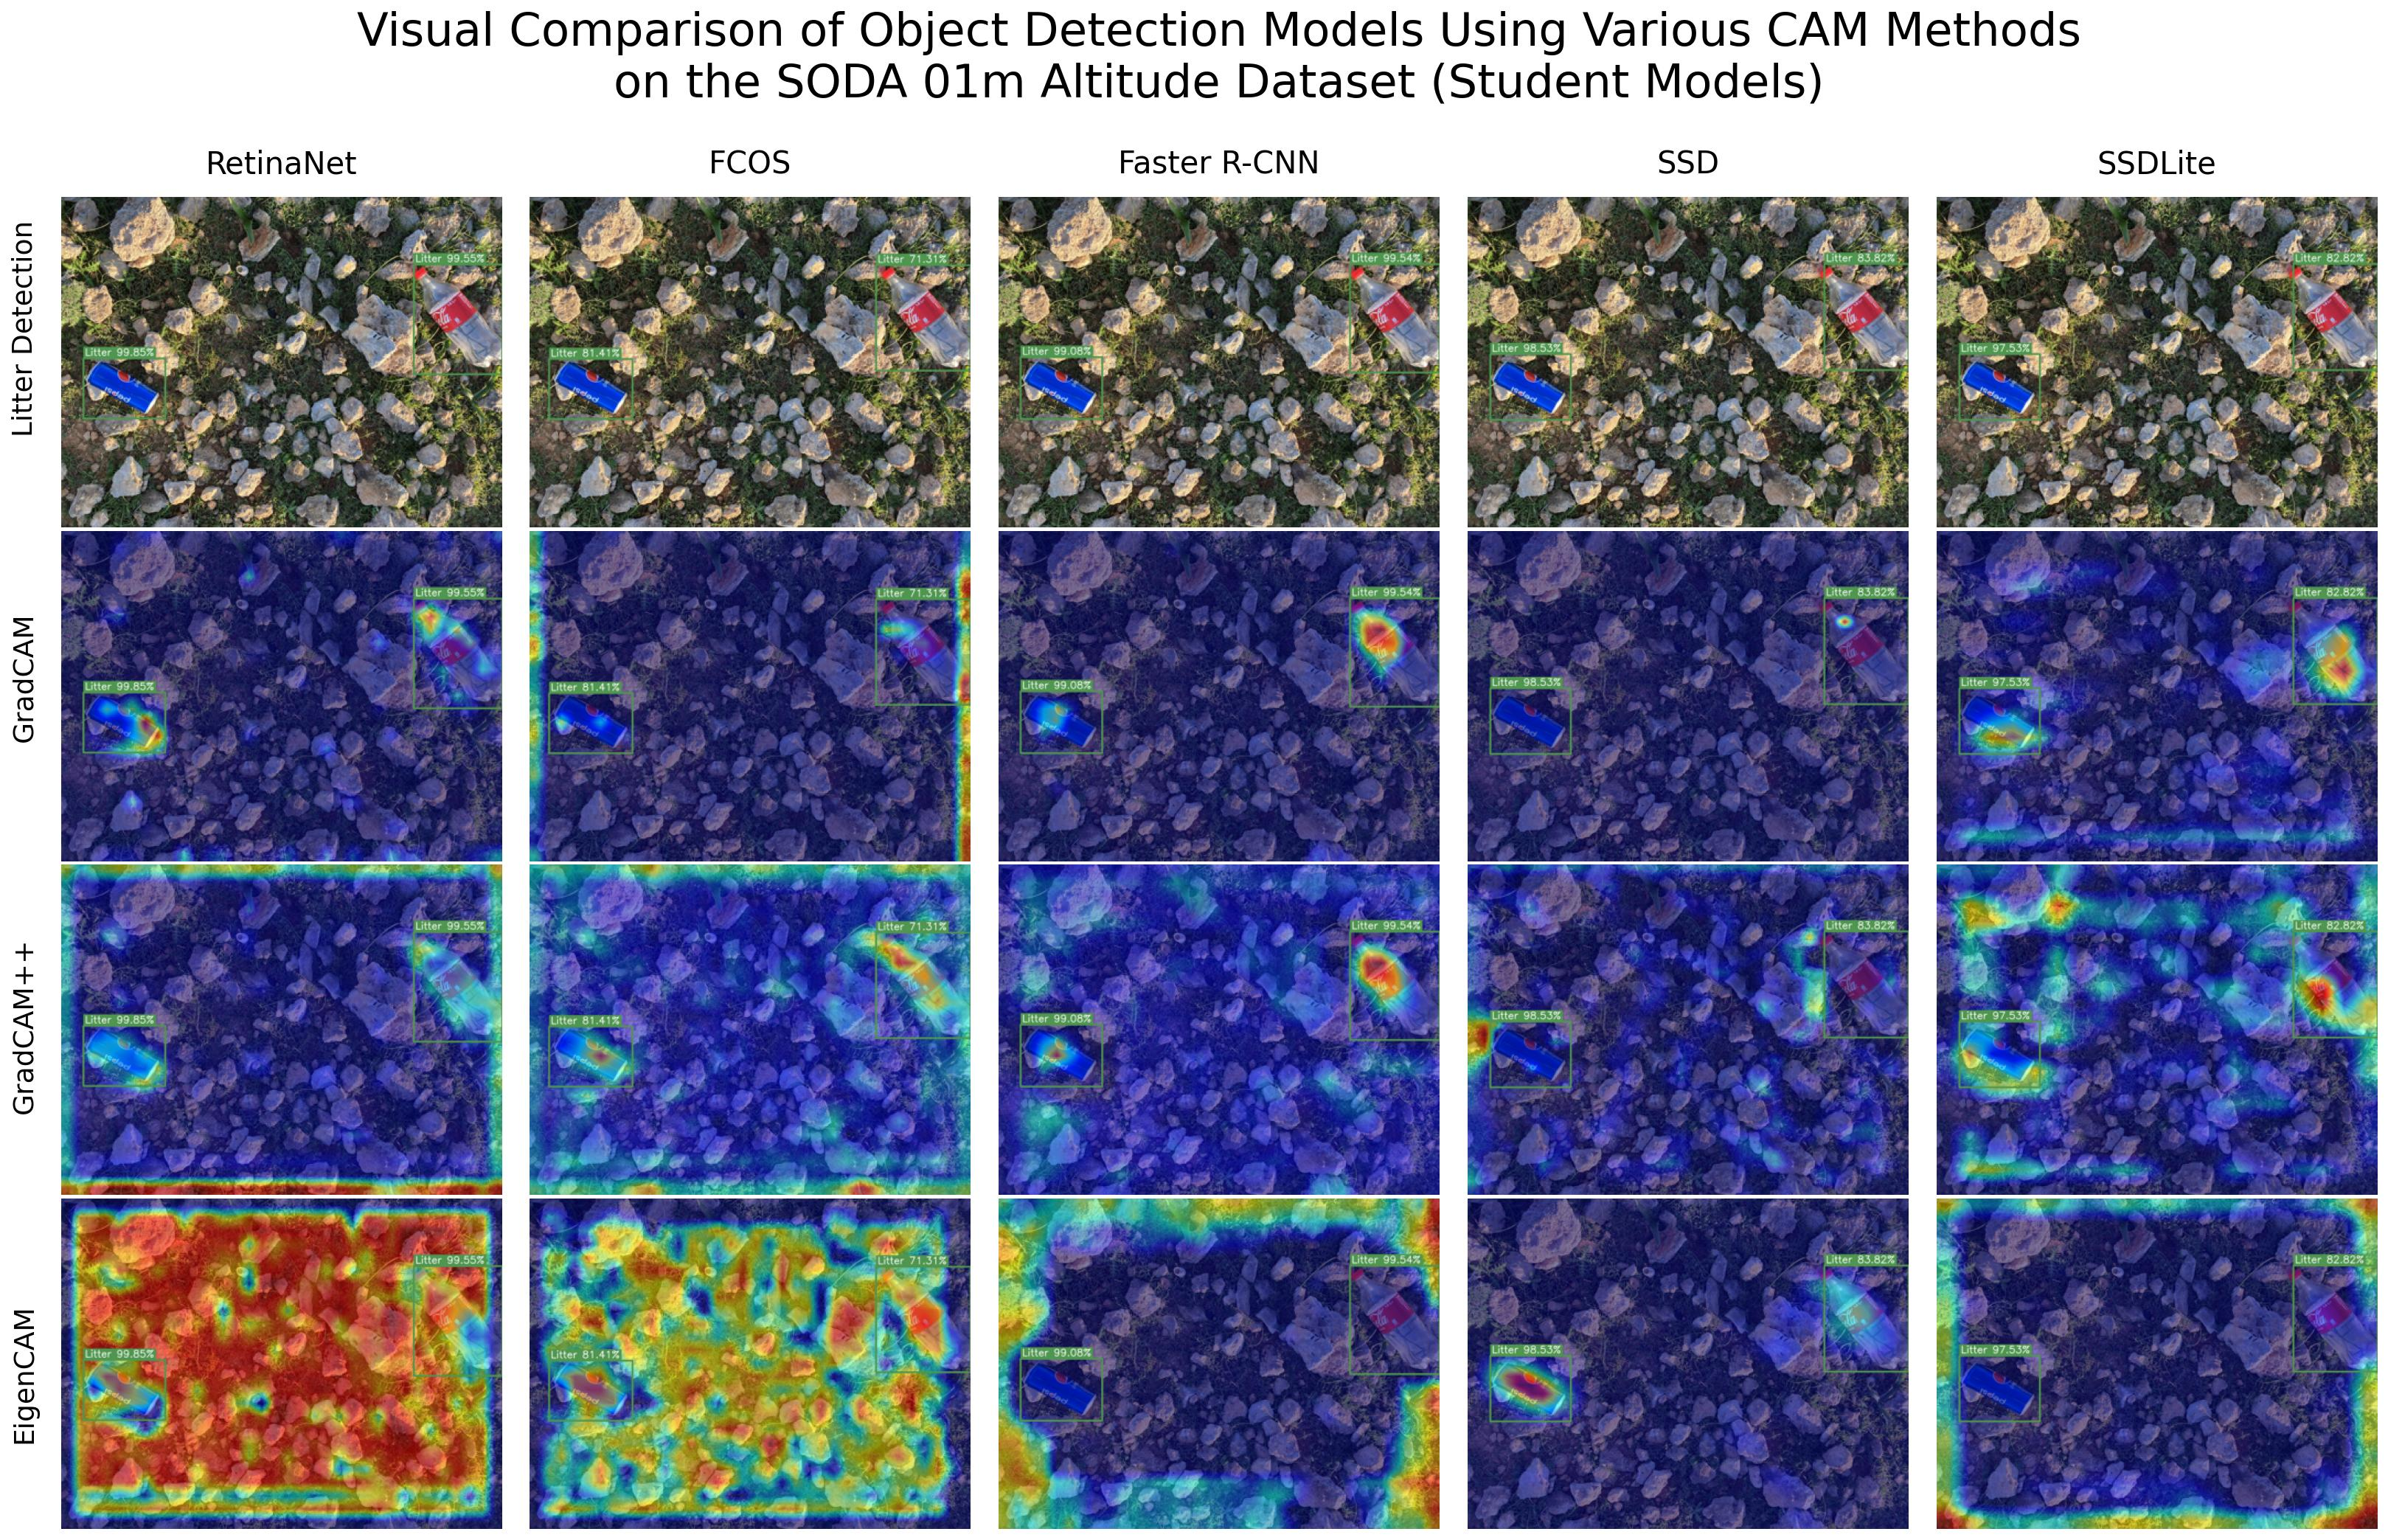
\includegraphics[width=0.9\textwidth]{gradcam_comparison_student.jpg} \\
        \small (b) \\
    \end{tabular}
    \caption{Visual comparison of object detection models using various \gls{cam} methods on the \gls{soda} dataset at a 1-metre altitude for binary litter detection. (a) shows predictions from baseline models; (b) presents predictions from the corresponding student models.}
    \label{fig:gradcam_comparison}
\end{figure}

A consistent trend observed in Section \ref{sec:5_visual_results} is also evident here, with the student models generally outperforming the baselines. For example, the Faster \gls{rcnn} baseline mistakenly identified rocks as litter, a mistake that the student model successfully corrected. Likewise, both the \gls{ssd} and SSDLite baseline models missed certain litter objects, while the student models successfully identified them.

Shifting the focus to the class activation maps, the visual differences between baseline and student models are more subtle. While the activation maps from Grad-\gls{cam}, Grad-\gls{cam}++, and Eigen-\gls{cam} are relatively similar in overall appearance, some meaningful observations can still be made. In the Grad-\gls{cam} outputs, even for objects that were not detected by the \gls{ssd} and SSDLite baselines, some degree of attention was still allocated to those regions. This suggests that although the models failed to classify the objects correctly, they were at least partially aware of their presence.

A consistent pattern across the baselines, particularly in scenes with rocky terrain, was the misallocation of attention. The models often focused on background elements such as rocks, which may have contributed to the misclassifications. In contrast, the student models appeared to suppress this background attention, instead concentrating more directly on the relevant object areas.

In the Grad-\gls{cam}++ results, the effect of the challenging backgrounds became even more evident. The baseline models directed substantial attention to the rocky textures rather than the actual litter, which likely impaired their predictions. The student models, however, showed a shift in behaviour: their attention was more evenly spread across the scene but still retained a clear focus on the objects of interest, avoiding the distractive influence of the background.

Finally, the Eigen-\gls{cam} results also show a difference in attention. The student models spread their focus more evenly across the entire image, including the object regions, without being sidetracked by the background. In contrast, the baseline models focused more on the litter objects. However, in this case, the baseline models did give more attention to the specific litter, while the student models seemed to distribute their attention more widely, including the background.

Looking at the results, the other trained detection models showed similar outcomes, supporting the same conclusion: the proposed \gls{lupi}-based method improves detection results while also guiding the models' attention more effectively. This ability to shift focus away from irrelevant background features and towards the objects of interest, while in cases of challenging backgrounds, dispersing attention across the whole image instead of fixating on specific background elements, appears to be a crucial factor in the improved performance of the student models.


\section{Limitations in Privileged Information Generation}
\label{sec:5_fail_cases_priv_info_gen}
% Madonna Itlob Ghalina u Ddefendina, ghal Dejjem ta' Dejjem. Amen. Grazzi

While it has been demonstrated that leveraging privileged information in object detection offers significant benefits, especially with simplified modifications and lightweight alternatives to complex architectures, it is also prudent to consider the limitations associated with this approach. One of the primary challenges lies in generating the privileged information itself. As previously acknowledged, the increased training time required for this method, compared to excluding privileged information, is a key drawback. However, there are still issues in effectively representing certain objects through this information.

These limitations can primarily be broken down into three key challenges: (i) overlapping objects of the same type, (ii) large objects obscuring smaller ones, and (iii) difficulties in distinguishing between object classes in datasets with a large number of categories. In the case of \gls{uav}-based litter detection, where litter items are relatively small and spaced apart, this method performs well (as seen in Figure \ref{fig:privileged_visual}). However, in scenarios with overlapping objects, the challenge of encoding privileged information becomes more pronounced.

Figure \ref{fig:fail_cases} illustrates three examples of these difficulties using the Pascal \gls{voc} 2012 dataset. In the first row, subfigure (a) shows an image of multiple chairs. The privileged information in subfigure (b) shows the bounding boxes merged together, making it challenging to distinguish the individual objects. This issue arises when objects overlap, leading to a lack of clarity in the privileged information. In the second row, subfigures (c) and (d) show a scene with several buses in the background, many of which are obscured by the aeroplane, one bus also partially hides a significant portion of the person in front of the plane, ultimately confusing detection. While this problem can be partially addressed through sorting, as was done in this study (refer to Algorithm \ref{alg:boundingBoxMask}), some smaller objects remain occluded by larger ones. Finally, in the third example (e) shows an image of a boy and a motorcycle, with the privileged information in (f) still distinguishing the two objects due to slight colour differences. However, this highlights a limitation when dealing with datasets that contain many object categories. The pool of distinct colours available to represent different objects becomes too small. A possible solution could be increasing the number of channels to use an RGB mask instead of a grayscale mask, but this would significantly increase training time.

\begin{figure}[!ht]
  \centering
  \begin{tabular}{cc}
    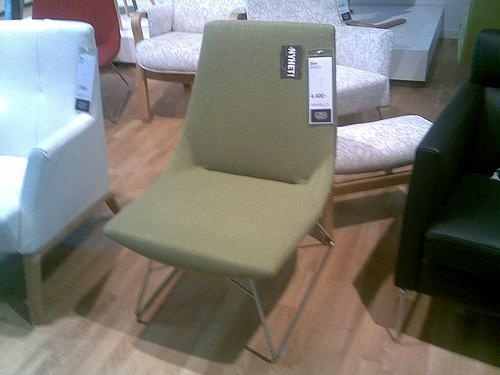
\includegraphics[width=0.47\textwidth]{fail_case1.jpg} &
    
\includegraphics[width=0.47\textwidth]{fail_case2.jpg} \\
    \small (a) & \small (b) \\
    \addlinespace[1em]
    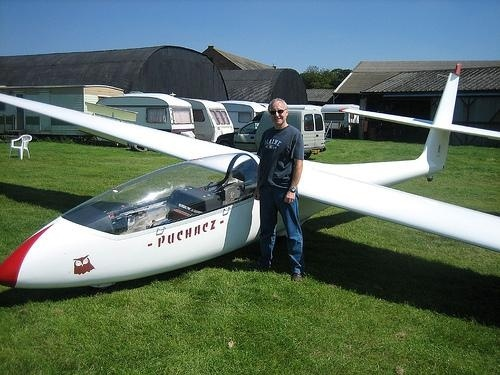
\includegraphics[width=0.47\textwidth]{fail_case3.jpg} &
    
\includegraphics[width=0.47\textwidth]{fail_case4.jpg} \\
    \small (c) & \small (d) \\
    \addlinespace[1em]
    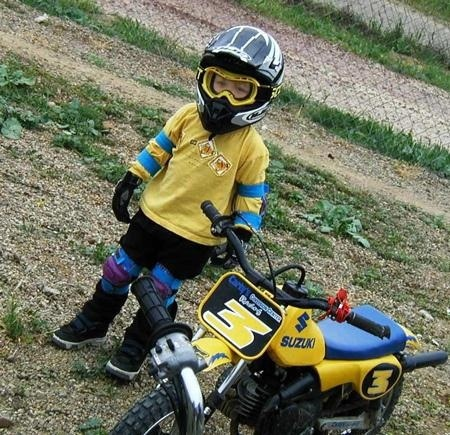
\includegraphics[width=0.47\textwidth]{fail_case5.jpg} &
    
\includegraphics[width=0.47\textwidth]{fail_case6.jpg} \\
    \small (e) & \small (f) \\
  \end{tabular}
  \caption{Examples of failure cases in privileged information generation. Subfigures (a), (c) and (e) show original images from the Pascal \gls{voc} 2012 dataset, while (b), (d) and (f) display the corresponding generated privileged information.}
  \label{fig:fail_cases}
\end{figure}

These examples highlight the limitations inherent in generating privileged information, particularly in encoding bounding box data for object detection networks. The difficulties become more pronounced in scenarios involving overlapping objects or complex scenes with numerous categories. While strategies such as sorting or expanding the colour pool may alleviate some of these issues, there remains a need for further investigation into how this method can be generalised for larger, more intricate use cases. Nevertheless, the advantages of employing this approach significantly outweigh its limitations, suggesting that continued research in this area is both necessary and valuable.

\section{Discussion}
\label{sec:5_discussion}
% Glorja lil Missier, lil Iben u lil Ispirtu s-Santu. Amen.

Having carefully examined the experimental results discussed earlier, it is appropriate to consider these outcomes in relation to the central research question. This study aimed to determine whether the integration of the \gls{lupi} paradigm could be effectively applied within object detection frameworks, and to assess the practical feasibility of doing so. To support this investigation, four specific objectives were drawn up. The first objective (\textbf{O1}) focused on evaluating the real-world applicability of the method, using the particularly demanding use case of litter detection as an example of small object detection. The second objective (\textbf{O2}) centred on implementing and testing the approach across a broad selection of established object detection models, in order to examine whether the proposed strategy could generalise across architectures with different design characteristics.

Objectives \textbf{O3} and \textbf{O4} extended the scope of evaluation. These focused on testing the method within a structured experimental design, both within individual datasets and across distinct datasets, to explore its efficacy in scenarios of increasing difficulty and environmental complexity. Particular attention was given to the trade-offs between detection accuracy and computational efficiency, both of which are key factors in assessing feasibility. The findings provide clear evidence that the proposed method consistently yielded improvements. Across three difficult within-dataset scenarios based on \gls{uav}-collected litter detection tasks, the \gls{lupi} trained student models outperformed baseline counterparts, with measurable improvements in detection accuracy.

Although the extent of improvement varied depending on the complexity of the task, with smaller accuracy observed in more challenging scenarios, the approach continued to demonstrate success. Preliminary experiments also explored the selection of optimal tiling parameters, contributing to the broader aim of determining feasibility within \gls{uav}-based litter detection use cases. Further evaluation focused on the method’s ability to generalise to external datasets, specifically \gls{bdw} and UAVVaste. These experiments once again confirmed that incorporating privileged information resulted in meaningful performance improvements. This outcome remained consistent even in cross-dataset evaluations, a setting where object detection models frequently encounter difficulties in maintaining accuracy.

The Pascal \gls{voc} 2012 dataset was subsequently employed to assess the method across a wider variety of object classes. The results demonstrated that the proposed approach maintained robustness even in more general-purpose object detection scenarios. Throughout the full set of experiments, five commonly used architectures were selected: Faster \gls{rcnn}, \gls{ssd}, RetinaNet, SSDLite, and \gls{fcos}. For each architecture, three model variants were trained: a baseline, a teacher, and four student models developed within the \gls{lupi} framework. Certain architectures, including RetinaNet and \gls{fcos}, yielded stronger results in \gls{uav}-based litter detection tasks, whereas SSDLite and \gls{ssd} achieved better performance in the Pascal \gls{voc} evaluation. Faster \gls{rcnn} demonstrated consistent performance across both contexts, although its relative advantage varied depending on the dataset and detection challenge. These outcomes suggest that differences in baseline performance are likely driven by the degree to which each architecture is suited to the characteristics of the target task, rather than by any inherent constraint of the \gls{lupi} approach.

In total, \textit{120} object detection models were trained and evaluated, which made it possible to conduct an ablation study on the \gls{alpha} parameter to identify optimal conditions for student model learning. Although the proposed approach leads to longer training times and some minor limitations in the privileged information generation, it does not impact the model size or the number of parameters. As a result, lightweight models remain suitable, as they can deliver improved accuracy while maintaining efficiency during inference. Since inference is typically performed far more frequently than training in most deployment scenarios, this trade-off is both practical and worthwhile.

Finally, visual outputs and feature-based analyses indicate that models trained with the proposed method can detect a greater number of objects with higher confidence. These models also exhibit stronger feature representations, further supporting the robustness of the approach. Overall, the findings suggest that the research question has been answered with a reasonable degree of confidence. The method demonstrates clear practical feasibility and measurable improvements in detection accuracy, particularly in scenarios where constraints on model size and inference speed are crucial, as in the case of \gls{uav}-based small object detection.


%--

\section{Conclusion}
\label{sec:5_conclusion}



%--

\begin{itemize}
    \item UREC Ethics Form - Done
    \item Problem Definition
    \item pages 110-120 maximum
    \item To check Daniel thesis
\end{itemize}

Evaluation
\begin{itemize}
    \item Tiling experiment - SODA include and exclude one meter magnification for SODA - Done

    \item Experiment 1 - Within dataset evaluation - Done
    \item Within dataset - 3 tas SODA Dataset - show all charts and tables + discussion - Done
    \item Across dataset - BDW and UAVVaste - Done
    \item Generalisation - Pascal VOC - Done
    \item Ablation studies - alpha for LUPI and Distillation (nest inside) - Done
    \item Visual Analysis, Ground truth, mask overlap, litter predictions
    \item Interpretability Grad CAM
    \item Discussion - Go over research question once more, theoretical aspect, Knowledge Distillation and Applications - Project AWIGS, summary
\end{itemize}

Conclusion
Revisting aims and objectives
limitation and future work (everything from future work goes here)
Conclusion

Future Work - Future Research/Future Projects
\begin{itemize}
    \item Trying out this method for Segmentation
    \item generalisation capabilities on Pascal VOC and COCO to ask what to include
    \item Test out the method on state-of-the art object deteciton architectures such as YOLO11 etc. . . - can be a limitation
    \item considerations of real time or alternatives to privileged information
    \item Improvement in terms of encoding the bounding boxes for the teacher better and iinvestigating in better channels etc. . . (to ask)
    \item further tests on generalisation of higher class datasets and training parameters
\end{itemize}

%--
